%----------------------------------------------------------------------------------------
%	PREAMBULE // PACKAGES AND OTHER DOCUME2NT CONFIGURATIONS
%----------------------------------------------------------------------------------------
\documentclass[a4paper,12pt,twoside,english]{book}
\usepackage[utf8]{inputenc}
\usepackage[T1]{fontenc}
\usepackage{babel}
% \usepackage[backend=biber]{biblatex}

%	MARGIN SETTINGS
\usepackage[a4paper,left=2cm,right=2cm,top=2cm,bottom=2cm, twoside]{geometry}

\usepackage{xcolor}
\usepackage{stmaryrd}
\usepackage{amssymb}
\usepackage{amsmath}
\usepackage{libertine}



%\usepackage{cite}
\usepackage{hyperref} % for references (\ref, \label), url
\hypersetup{
    colorlinks=true,
    linkcolor=black,
    filecolor=black,      
    urlcolor=black,
    citecolor=black,
    pdfpagemode=FullScreen,
    }
\usepackage[
    % backend=biber, 
    natbib=true,
    style=numeric,
    sorting=none
]{biblatex} %Imports biblatex package

\addbibresource{biblio.bib} %Import the bibliography file

\usepackage{graphicx} % to include images
%\usepackage[pdftex]{graphicx}
\graphicspath{ {figures/} }
\usepackage{caption}
\usepackage{subcaption}
\usepackage{float}
\usepackage{multirow}
\usepackage{array, multirow, tabularx}
\usepackage{booktabs}
\usepackage{longtable}
\usepackage{apalike}
\usepackage{minitoc}
\usepackage{tikz}
\usepackage{fancyhdr}
\pagestyle{fancy}
\usepackage[strict]{changepage}
\usepackage{siunitx}
\selectlanguage{english}%

\usepackage{enumitem}
\usepackage{epigraph}
%\usetikzlibrary{shadows.blur}
\usepackage{lscape}
\usepackage{titletoc}
\usepackage{mdframed}

\usepackage{tabu}
\usepackage{pdfpages}

\usepackage{arydshln}
%\usepackage[nonumberlist]{glossaries}
\usepackage{calc}
\usepackage[]{titlesec} 
\definecolor{linkColor}{HTML}{32a852}
%\usepackage[colorlinks=true,citecolor=linkColor,linkcolor=black]{hyperref}

\addto\captionsfrench{%
  \renewcommand{\listfigurename}{List of figures}%
}



%%%%%%%%%%%%%%%%%%%%%%%%%%%%%%%%%%%%%%%%%%%%%%%%%%%%%%%%%%%%%%%%%%%%%%%%%%
%%%%%%%%%%%%%%%%%%%%%%%%%%%%%%%%%%%%%%%%%%%%%%%%%%%%%%%%%%%%%%%%%%%%%%%%%%

\usepackage{sectsty}
%\sectionfont{\color{CentraleRed}}  % sets colour of sections
%\subsectionfont{\color{uclablue}}  % sets colour of subsections, ou gray, teal 
\definecolor{darkseagreen}{rgb}{0.56, 0.74, 0.56}
\usepackage{lipsum}

\title{INSATIABLE V2.0.}
\author{EYANGO TABI Loic}
\date{March 2025}


%----------------------------------------------------------------------------------------
%	HEADERS AND FOOTERS
%----------------------------------------------------------------------------------------

%\fancyhead[RO]{\scshape \leftmark}
%\fancyhead[L]{\scshape \righttmark}
\fancyhead{} % clear all header fields
\fancyfoot{} % clear all footer fields
%\fancyhead[LE,RO]{\slshape \rightmark}
\fancyfoot[C]{--~\thepage~--}

\usepackage{emptypage}

%\leftmark : adds name and number of the current top-level structure (for example, Chapter for reports and books classes; Section for articles ) in uppercase letters.
% \rightmark : adds name and number of the current next to top-level structure (Section for reports and books; Subsection for articles) in uppercase letters.

%%%%%%Glossaire
%\usepackage{glossaries}
\usepackage[acronym,xindy,toc]{glossaries} % nomain, if you define glossaries in a file, and you use \include{INP-00-glossary}
%[nomain,acronym,xindy,toc]
\makeglossaries

\usepackage[xindy]{imakeidx}
\makeindex
%\input{auxilliaires/glossaire}
%%%%%%%%%%%%%%%%%%%%%%%%%%%%%%%%%%%%%%%%%%%%%%%%%%%%%%%%%%%%%%%%%%%%%%%%%%
%%%%%%%%%%%%%%%%%%%%%%%%%%%%%%%%%%%%%%%%%%%%%%%%%%%%%%%%%%%%%%%%%%%%%%%%%%
%----------------------------------------------------------------------------------------
%	DOCUMENT
%----------------------------------------------------------------------------------------

\begin{document}

    \begin{titlepage}
        %\maketitle
        %----------------------------------------------------------------------------------------
        %	TITLE PAGE
        %----------------------------------------------------------------------------------------
        
\includepdf[pages=1]{figures/ED_requirements/page_de_garde.pdf}  % Replace with your actual filename
        \newpage %passer à une nouvelle page
        \thispagestyle{empty} %page de garde vide
    \end{titlepage}
    
%\renewcommand{\chaptermark}[1]{\markboth{\textsc{#1}}{}}
\renewcommand{\chaptermark}[1]{\markboth{#1}{}}
\frontmatter % numérote les pages en chiffres romains jusqu'a la commande mainmatter

%----------------------------------------------------------------------------------------
%	RESUME ET ABSTRACT PAGE
%----------------------------------------------------------------------------------------
 

%----------------------------------------------------------------------------------------
%	QUOTATION PAGE ou DEDICACE
%----------------------------------------------------------------------------------------
\clearpage
\vspace*{0.2\textheight}


\begin{quote}
\textbf{
"La connaissance s'acquiert par l'expérience, tout le reste n'est que de l'information".
}
\end{quote} \bigbreak

\hfill 
- Albert Einstein (n.d.)



% \mbox{}
% \newpage
%----------------------------------------------------------------------------------------


%----------------------------------------------------------------------------------------
%	ACKNOWLEDGEMENTS
%----------------------------------------------------------------------------------------
\chapter*{Remerciements}
\addcontentsline{toc}{chapter}{Remerciements}

Cette thèse n’aurait pu voir le jour sans l’accompagnement, le soutien et l’expertise de nombreuses personnes, que je tiens à remercier ici chaleureusement. \vspace{0.5\baselineskip}

Je souhaite tout d’abord exprimer ma profonde gratitude à mes encadrants académiques, \textbf{Sébastien PICAULT} et \textbf{Nicolas PARISEY}, pour leur engagement sans faille tout au long de ce travail. Leur patience, leur polyvalence, ainsi que la richesse de leurs connaissances et de leur expertise ont constitué un cadre intellectuel stimulant, exigeant et toujours bienveillant. Leur regard croisé a permis à ce projet de s’épanouir à l’intersection de plusieurs disciplines, en lui donnant à la fois rigueur scientifique et portée opérationnelle. \vspace{0.5\baselineskip}

Je remercie également mes encadrants en entreprise, \textbf{Xavier L'HOSTIS} et \textbf{Victoria POTDEVIN}, dans le cadre de la convention CIFRE, au sein d’\textbf{Adventiel}. Leur disponibilité, leur écoute, et leur capacité à prendre du recul sur les cas d’usage concrets ont grandement contribué à l’ancrage et à la pertinence de ce travail. Leur bienveillance, leur patience et le temps qu’ils m’ont consacré m’ont permis d’évoluer sereinement dans un environnement professionnel exigeant mais toujours ouvert. Je n'oublie évidemment pas non plus \textbf{Jean DU PUYTISON}, qui a su me faire confiance et a soutenu le projet.\vspace{0.5\baselineskip}

Je tiens à adresser mes remerciements sincères à l’ensemble de l’équipe DATA  d’\textbf{ADVENTIEL}, en particulier \textbf{Léane}, \textbf{Bastien}, \textbf{Tim} et tout spécialement \textbf{Leslie}, pour leur soutien constant, leur temps précieux et leurs relectures attentives du manuscrit, qui m’ont grandement aidé dans les dernières phases de rédaction. Un grand merci à \textbf{Lila}, sans qui je n'aurais jamais réussi toutes les démarches administratives ainsi qu'à \textbf{Maxime} et \textbf{Nathan} pour leur bonne humeur. \vspace{0.5\baselineskip}

Mes remerciements s’adressent également à l’équipe \textbf{DYNAMO de BIOEPAR} : \textbf{Gaëlle}, \textbf{Halifa}, \textbf{Pauline}, \textbf{Baptiste}, \textbf{Guita} et \textbf{Vianney}, pour leurs relectures précieuses, leurs retours constructifs et la qualité de leurs apports scientifiques spécifiques, qui ont enrichi le projet à bien des égards. \vspace{0.5\baselineskip}

Un grand merci à l’équipe d’\textbf{ONIRIS}, et en particulier à \textbf{Sébastien ASSIE} pour son soutien, ainsi qu’à \textbf{Maud}, pour le temps considérable qu’elle a consacré à la relecture des articles, à son expertise vétérinaire et à la collecte et l’annotation des données dans des conditions parfois difficiles. Son implication concrète a été essentielle à la robustesse des résultats présentés. \vspace{0.5\baselineskip}

Je tiens à exprimer toute ma reconnaissance à mes amis et à ma famille, en particulier à \textbf{Vianney}, \textbf{Mathurin}, \textbf{Nadia} dont le soutien inébranlable m’a été d’un précieux secours tout au long de ce parcours. \vspace{0.5\baselineskip}

Enfin, je souhaite remercier chaleureusement mes chers \textbf{parents} pour leur soutien indéfectible et leur présence, même à distance. Leur appui constant a constitué une source inestimable de force et de sérénité durant les moments difficiles. \vspace{0.5\baselineskip}

Bien que la liste soit encore bien plus longue, j'exprime ma plus sincère gratitude à toutes ces personnes, ainsi qu'à celles qui ont croisé mon chemin, de près ou de loin, tout au long de cette thèse.



%----------------------------------------------------------------------------------------
%	LIST OF CONTENTS/FIGURES/TABLES PAGES
%--------------------------------------------------‡--------------------------------------
\setcounter{secnumdepth}{3} % organisational level that receives a numbers
\setcounter{tocdepth}{3}
\tableofcontents % Prints the main table of contents
\listoffigures % Prints the list of figures
\addcontentsline{toc}{chapter}{List of figures}
% \listoftables % Prints the list of tables
% \addcontentsline{toc}{chapter}{List of tables}

%----------------------------------------------------------------------------------------
%	Liste des abréviations-
%----------------------------------------------------------------------------------------
%\chapter*{Liste des abréviations}
%\addcontentsline{toc}{chapter}{Liste des abréviations} 

\printglossary[type=\acronymtype, title=List of abbreviations,toctitle=List of abbreviations]

\newglossaryentry{latex}
{
        name=latex,
        description={Is a mark up language specially suited for 
scientific documents}
}


\newacronym{RTN}{RTN}{Rat-Taupe Nu}

\newacronym{IUCN}{IUCN}{Union Internationale pour la Conservation de la Nature}

\newacronym{ENVA}{ENVA}{Ecole Nationale Vétérinaire de maison Alfort}

\newacronym{JDE}{JDE}{Jonction Dermo-Épidermique}

\newacronym{MB}{MB}{Membrane Basale}




% --------------------------------------------------------------
%                         Début du corps
% --------------------------------------------------------------

\mainmatter
\setlength{\parskip}{.7em}

%\titlespacing*{\section}{0pt}{.9em}{.8em}
\renewcommand{\baselinestretch}{1.1}

\fancyhead[RO]{\leftmark}
\fancyhead[LE]{\textsc{\chaptername~\thechapter}}

%\chapter*{Introduction}
% \fancyhead{} % clear all header fields
% \fancyhead[OL]{\textsc{Foreword}}
% \chapter*{Foreword - à enlever !} % Main chapter title
\addcontentsline{toc}{chapter}{Foreword}  

%Le but de l'avant-propos est d'améliorer les conditions dans lesquelles les membres d’un jury, vont pouvoir l’apprécier.
%\textbf{C’est une partie facultative du travail de recherche dans laquelle l’auteur peut expliquer les raisons qui l’ont incité à étudier le sujet en question, tout en exposant le but poursuivi et les difficultés rencontrées en cours de recherche.}

The conjoining of dynamical systems and deep learning has become a
topic of great interest. In particular, neural differential equations (NDEs)
demonstrate that neural networks and differential equation are two sides
of the same coin. Traditional parametrised differential equations are a
special case. Many popular neural network architectures, such as residual
networks and recurrent networks, are discretisation.
NDEs are suitable for tackling generative problems, dynamical systems,
and time series (particularly in physics, finance, . . . ) and are thus of
interest to both modern machine learning and traditional mathematical
modelling. NDEs offer high-capacity function approximation, strong priors
on model space, the ability to handle irregular data, memory eficiency,
and a wealth of available theory on both sides.
This doctoral thesis provides an in-depth survey of the field.
Topics include: neural ordinary differential equations (e.g. for hybrid
neural/mechanistic modelling of physical systems); neural controlled differential
equations (e.g. for learning functions of irregular time series);
and neural stochastic differential equations (e.g. to produce generative
models capable of representing complex stochastic dynamics, or sampling
from complex high-dimensional distributions).
Further topics include: numerical methods for NDEs (e.g. reversible
differential equations solvers, backpropagation through diferential equations,
Brownian reconstruction); symbolic regression for dynamical systems
(e.g. via regularised evolution); and deep implicit models (e.g. deep
equilibrium models, differentiable optimisation).
We anticipate this thesis will be of interest to anyone interested in the
marriage of deep learning with dynamical systems, and hope it will provide
a useful reference for the current state of the art.



\subsubsection*{Motivation}

We have two goals in writing this document. One: to satisfy the requirements of a
PhD, by writing a thesis describing our original research. Two: to give an accessible
survey of the new, rapidly developing, and in our opinion very exciting field of neural
differential equations. To the best of our knowledge this is the first survey to have
been written on the topic.
We hope this will prove useful to the interested reader! Along the way we shall cover a
wide variety of applications, both to classical mathematical modelling, and to typical
machine learning problems.


\subsubsection*{Getting started}
We will assume throughout that the reader is familiar with the basics
of ODEs and with the basics of modern deep learning, but we will not assume an
in-depth knowledge of either. On the basis that many of our readers may come from a
traditional applied mathematics background without much exposure to deep learning,
then Appendix A also provides a summary of the relevant deep learning concepts we
shall assume. It also provides references for learning more about deep learning.
The material on neural SDEs will assume familiarity with SDEs.
Beyond these (relatively weak) assumptions, we will introduce concepts as we need
them. Various parts of the text will touch on topics such as rough path theory,
or numerical methods for differential equations. In each case we assume little-tono
familiarity on the part of the reader, and where necessary provide references for
learning more about them.
The next chapter (on neural ODEs) makes an effort to explicitly spell out even `elementary'
details such as the existence of solutions to ordinary differential equations,or the use of cross entropy as a loss function. Later chapters assume increasing levels
of sophistication; it is recommended to read them in sequential order.

Code The reader interested in applying these techniques is strongly encouraged to
write some example code.
Each chapter contains a few numerical examples usually on toy datasets for ease
of understanding. The corresponding code is both available and well-documented:
they can be found as the examples of the Diffrax software library [Kid21a], which is
written for the JAX framework [Bra+18].
Indeed standard software libraries for solving and differentiating differential equations
make working with NDEs essentially easy. These are discussed in Section 5.6
(including both Diffrax and other options for other frameworks). These libraries are
again well-documented and contain numerous examples.


Experiments The material here focuses on presenting the theory of NDEs; correspondingly
our numerical examples will tend to be on toy datasets chosen for ease of
understanding. Real world (and possibly very large scale) applications of these techniques
may be found in the original papers, which are referenced in the text alongside
each individual topic.


\textcolor{red}{je dois rajouter une partie pour les notations scientifiques/mathématiques ? comme la thèse "On neural differential equations". partie appélé "Notations"}
 %avant-propos

\fancyhead{} % clear all header fields

\fancyhead[RO]{\leftmark}
\fancyhead[LE]{\textsc{\chaptername~\thechapter}}

\chapter{Introduction} 

\section{Livestock farming, animal health and infectious diseases}

% [\textcolor{red}{A update une fois que j'aurai fini cette section}]
Livestock farming today is embedded in a complex socio-economic landscape that underpins food security, rural development, and environmental sustainability. As global populations rise and resource constraints become more acute, the ability to produce high-quality animal products in a sustainable manner is more critical than ever. This sector not only ensures the availability of nutritious food but also supports the livelihoods of countless rural communities, thereby reinforcing local economies. In parallel, the modern challenges of animal health and public safety are converging, with infectious diseases emerging as a significant threat that jeopardizes both the productivity of farming systems and the broader public health framework. The traditional approach to livestock management, which often treats animal health in isolation, is increasingly being questioned in favour of a more integrated strategy that acknowledges the intricate links between animal welfare, human well-being, and environmental health.

In this context, infectious diseases are not merely biological phenomena but are embedded within the socio-economic fabric of livestock farming. Their impact reverberates through production losses, escalating veterinary expenses, and the overuse of antibiotics, which in turn contribute to public health concerns such as antimicrobial resistance. These challenges demand a rethinking of conventional control measures and underscore the urgency of developing sustainable farming practices that can adapt to both immediate crises and long-term environmental pressures. By embracing an integrated approach, the sector can transform these challenges into opportunities for innovation, leveraging advanced technologies and interdisciplinary strategies to enhance animal health, protect public well-being, and ensure the economic viability of farming systems for future generations.

This section provides a comprehensive overview of the socio-economic landscape that surrounds livestock farming, underscoring its importance for food security, public health, environmental management, and the integrated “One Welfare” approach. It section also highlights key challenges related to the impact of infectious diseases on livestock farming as well as conventional methods used to diagnose, manage, and prevent these diseases and their inherent limitations.

\subsection{Socio-economical context and the stakes}



% Finally, the rationale for integrating new, data-driven modelling approaches is introduced, emphasizing their potential to improve disease surveillance and decision-making. These methods aim to complement the expertise of farmers and veterinarians by providing more accurate prognostics, optimizing resource use, and ultimately contributing to more resilient and welfare-focused livestock farming systems.

\subsubsection{Livestock Farming, animal health well-being}

Livestock farming constitutes a cornerstone of global agriculture, underpinning food security and rural development while driving significant economic contributions worldwide (Fig \ref{fig:chap1-livestock}). In Europe, the average livestock farm covers approximately 34 hectares and maintains a herd size of around 47 livestock units, a scale that reflects both intensive production and resource management practices \cite{INRA_Livestock_Production}. Globally, the sector contributes up to 50\% of the agricultural gross domestic product and supports the livelihoods and food security of nearly 1.3 billion people in developing countries, highlighting its critical role in sustaining rural economies \cite{Herrero2016, FAO2017}

The environmental footprint of livestock farming is also considerable. Livestock production occupies nearly 75\% of the agricultural land, underscoring its extensive spatial demands and the pressure it exerts on natural ecosystems \cite{Steinfeld181371}. High animal densities in confined feeding operations lead to substantial nutrient emissions, with studies reporting significant releases of nitrogen and phosphorus into the environment, thereby contributing to issues such as greenhouse gas emissions and water eutrophication \cite{Ramankutty2018, Mallin2015, LI2016451}


\begin{figure}[h]
  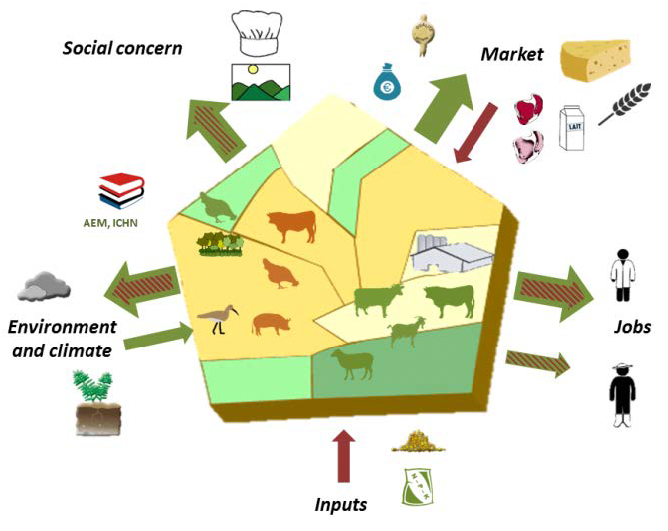
\includegraphics[width=\linewidth]{figures/chap1/chap1-livestockfarming.png}
  \caption{Bundle of services in areas with both crop and livestock farming. Illustration from \cite{INRA_Livestock_Production}}
  \label{fig:chap1-livestock}
\end{figure}

Future projections indicate a continuing rise in global demand for animal products, a trend driven by the so-called "livestock revolution" that accompanies increasing incomes and population growth, particularly in emerging economies \cite{Delgado2016}. This anticipated growth in demand is set against the backdrop of an already extensive current offer, where production scales and market dynamics are closely intertwined. Furthermore, livestock production accounts for about 15\% of global greenhouse gas emissions, with ruminants being the primary contributors due to their lower feed conversion efficiencies \cite{Gerber2013}. These figures underscore the urgency of balancing the expanding demand with sustainable production practices that safeguard both environmental quality and public health.

Animal health and welfare remain central to the sustainability of livestock farming systems. Societal concerns over animal well-being are driven not only by ethical considerations but also by the direct links between robust animal health, food safety, and public health outcomes. Ensuring high standards of animal welfare enhances productivity by improving feed conversion efficiency and reducing culling rates, while also reinforcing consumer trust in the safety and quality of animal products \cite{FAO2017}.

One of the major pressures on livestock farming is infectious diseases. These diseases challenge animal health and welfare, threaten food security and public health, and raise ecological concerns. The following subsection provides a brief overview of infectious diseases, detailing their intricate relationship with the environment and their overall impact on livestock systems.


\subsubsection{Livestock infectious diseases}

Bernard Vallat, Director General of the World Organisation for Animal Health (OIE), emphasized the escalating challenges posed by infectious diseases by stating, “As a result of globalisation and climate change, we are currently facing an unprecedented worldwide impact of emerging and re-emerging animal diseases and zoonoses (animal diseases transmissible to humans)” \cite{vallat2007protecting}. Indeed, infectious diseases represent a significant threat to livestock farming, deeply intertwined with environmental, economic, and public health factors. These diseases are caused by pathogenic microorganisms including bacteria, viruses, fungi, and parasites, capable of spreading directly or indirectly among animals, across species barriers (zoonoses), or through contaminated environmental media such as soil, water, or feed. Infectious disease has been chosen for consideration because globally these diseases have historically been, continue to be, and are expected to remain major concerns in the future. The increasing intensification of modern animal husbandry has encouraged the proliferation of infectious diseases and resulted in the emergence and increased importance of so-called multifactorial diseases.

Within livestock systems, infectious diseases manifest in diverse forms and can be categorized by their clinical presentations and modes of transmission. Respiratory infectious diseases, notably bovine respiratory disease complex and contagious bovine pleuropneumonia, pose substantial threats due to their rapid spread and significant economic impacts. Gastrointestinal infections such as salmonellosis and coccidiosis critically impair animal health and productivity through severe digestive disruptions. Bloodstream infections, exemplified by African swine fever, are particularly devastating due to their rapid progression, high mortality rates, and significant implications for international trade. Vector-borne diseases like bluetongue, transmitted by biting midges, are increasingly problematic in regions experiencing climate change, altering vector habitats and expanding disease ranges. Skin infections, including dermatophytosis and footrot, impose chronic health and welfare issues, severely affecting productivity and animal product quality \cite{gilbert2024quantifying}

The economic repercussions of infectious diseases in livestock are substantial, with diseases such as African swine fever and bovine tuberculosis significantly reducing productivity and incurring considerable veterinary costs \cite{gilbert2024quantifying}. Moreover, globalization, climate variability, and intensive farming practices further facilitate pathogen proliferation and dissemination, amplifying the scale and severity of outbreaks. Historical translocation events have dramatically demonstrated this potential, with diseases such as rinderpest and foot-and-mouth disease causing severe disruptions to global livestock production and trade \cite{GUMMOW201041}. Additionally, the widespread emergence of antibiotic resistance, driven by excessive antibiotic use in animal agriculture, poses critical challenges to effective disease management, raising serious concerns for animal welfare and health due to therapeutic failures \cite{bengtsson2014antibiotic}. To mitigate these threats, conventional control measures have and still play a employed, which are explored in the following subsection.


\subsection{Conventional control strategies of infectious diseases}
\label{Conventional control strategies} % ajout-du-label-pour-faire-reference-a-la-sous-section

Conventional control strategies for managing infectious diseases in livestock primarily rely on accurate diagnosis and prognosis to mitigate outbreaks and prevent their spread. Diagnosis involves identifying diseases through clinical appraisal, visual and tactile assessments conducted by farmers and veterinarians—and biological examinations, including laboratory analyses like PCR tests on collected samples. Prognosis entails predicting the potential progression and impact of identified diseases based on expert knowledge, historical data, and empirical observations. These methods culminate in tailored control recommendations, such as vaccination, quarantine, biosecurity protocols, and prudent use of antimicrobials. Given that livestock farming heavily utilizes natural resources, it is imperative to raise animals using best practices and innovations aimed at producing more with fewer inputs, including reduced use of water, land, feed, antibiotics, and waste. Livestock effluents, rich in organic matter, nutrients, pharmaceuticals, and heavy metals—can negatively affect ecosystems by contaminating soil and water bodies, accelerating eutrophication, and fostering antibiotic-resistant bacteria \cite{almeida2017veterinary, girard2014review, hooda2000review, martinez2009livestock}. Consequently, effective conventional disease control strategies are vital not only for animal welfare but also for preserving environmental health and public safety.

Despite their widespread adoption, conventional control methods possess inherent limitations, presenting significant challenges in practical livestock management. Clinical appraisal, although efficient and quick, is notably subjective and prone to inconsistencies between observers. Biological examinations, despite their precision, often introduce substantial delays and costs, rendering them less suitable for rapid decision-making during acute outbreaks. Scalability becomes problematic as livestock farming intensifies, with large-scale epidemiological surveillance demanding substantial human, financial, and logistical resources. The COVID-19 pandemic has starkly illustrated the importance of proactive risk management in infectious disease outbreaks, highlighting the necessity to better understand the mechanisms that influence disease emergence and severity. In parallel, broader societal debates challenge the sustainability of current livestock production practices, questioning the dominant productivist model and encouraging transitions toward more sustainable and integrative frameworks such as "ecological intensification," precision livestock farming utilizing transmitters, robotics, and statistical analyses, and agroecology, which relies on ecosystem services. These approaches aim to reconcile productivity demands with the critical need to manage environmental impacts responsibly \cite{INRA_Livestock_Production}. Consequently, there is a growing urgency to adopt automated, and integrative methodologies capable of overcoming the complexities inherent in infectious disease management, an area where precision artificial intelligence, epidemiology and data science could offer promising avenues for innovation and sustainability.  

%%%%%%%%%%% a rajouter dans le texte si ce n'est pas fait
% A major problem for the next 10 yr is the continuous monitoring of animal health within the big groups of animals. Due to the increasing number
% of animals and the decreasing number of farmers, every farm will count
% more animals. In the future, a single farm (or animal city) could see 25,000 milking cows, 200,000 fattening pigs, or a few million broilers. Infections in such big groups will have disastrous consequences while the reduction of the use of antibiotics is a primary challenge. The development of vaccines will take time, and the efficiency of applying vaccines in big herds must be monitored to improve them. Animal health is a top priority in relation to human health. In Europe, more than 25,000 people died due to not responding to antibiotics anymore while treatments cost of €1.5 billion (Anne Mottet, FAO, unpublished).The big density of animals living so close to humans in some countries is another issue. The number of zoonosis diseases that can be transferred to humans is very high. The safety and quality of the food products must be guaranteed at every moment. Another huge problem to be solved is the environmental impact of the livestock sector.


% et regrader de le docs de maud si on parle de méthode traditionnele de control des maladies infectieuse: éleveur comme vétos.
% je vais devoir chercher les chiffres pour argumenter certains faits. example: ethical concerns...



%----------------------------------------------------------------------------------------
%	SECTION 
%----------------------------------------------------------------------------------------
% \clearpage 


\section{Artificial intelligence, epidemiology and data science}

Artificial Intelligence (AI) is the study of computer systems designed to perceive their surroundings, think logically, learn from experiences, and take appropriate actions, essentially mimicking or enhancing human intelligence \cite{russell2020artificial}. Over time, AI has changed significantly. Early approaches focused on logic-based systems that relied heavily on explicit rules  \cite{nilsson2009quest}. Today, AI also uses machine learning, a method where algorithms automatically discover patterns directly from large amounts of observations \cite{Goodfellow-et-al-2016}.

Epidemiology is the study of how diseases spread in populations, what causes them, and how they can be controlled. A central idea in both epidemiology and AI is modelling. Modelling means creating simplified mathematical or computational representations of complex real-world phenomena to better understand, predict, and manage them. In epidemiology, models help scientists describe how diseases spread, predict how outbreaks might evolve, and guide effective public health responses \cite{keeling2008modeling}.

Regardless of the chosen modelling approach, the initial step always involves allowing the model to accurately perceive and interact with its environment. In livestock farming, this essential step is achieved through the use of sensors. These sensors can track animal behaviour, physiological parameters, location, and environmental conditions, enabling continuous monitoring of animal health and facilitating the early detection of diseases \cite{berckmans2017general}. Sensor-derived data can then feed into various modelling methods used in artificial intelligence to support decision-making. In this thesis, we particularly focus on two modelling paradigms: epidemiological mechanistic models, which rely on detailed knowledge of disease dynamics, and deep learning models, which automatically learn complex patterns directly from sensor data.


% Data science acts as a critical bridge, transforming vast observational data, such as health records, environmental conditions, and sensor readings—into actionable insights that inform epidemiological understanding and public health decisions.

% [Même si tu détailleras cela plus tard dans la thèse, indique déjà les perspectives que cela ouvre pour optimiser la prévention et le contrôle des maladies respiratoires. ]



\subsection{Precision livestock farming: sensors and observations}


% [from General introduction to precision livestock farming - D. berckmans]
% It has become impossible for farmers to follow all of their animals in a reliable way in such big groups. At the same time, several issues must be solved now in the livestock sector, such as monitoring animal health and welfare, reducing the environmental impact, and assuring the productivity of the process. Precision livestock farming (PLF) aims to offer a monitoring and managing system for farmers. This is fundamentally different from other approaches that tried to monitor the animal welfare by human  scoring animal-based indicators. These methods are not efficient to enough to improve the life of the animal under consideration. It is nice to detect a problem after an animal has arrived at the slaughterhouse, but it is much better to detect a problem while the animal is being reared and to take immediate management action. The idea of PLF is to provide a warning when something goes wrong so that immediate action can be taken by the farmer to solve the problem. 


% [positional data: ajouter colliers GPS (ex : chronopature ), les boucles permettent aussi l'identification des animaux]
% [operational data: tu ne parles pas des données issues de logiciels de gestion d'élevage (données d'identification, de production, cahier sanitaires, données génétiques : inséminations …)  ou de matériels installés type robot de traite]

Precision livestock farming (PLF) represents a technological shift aimed at improving livestock management by continuously monitoring animal health, welfare, and productivity through automated sensor systems. Driven by economic pressures, livestock farms have increasingly scaled up, leading to challenges in maintaining close and accurate animal monitoring through traditional methods. Consequently, PLF technologies have become integral for bridging the widening gap between animals and farmers \cite{NORTON20193009}.

The integration of sensor technology into livestock farming encompasses several categories. Behavioural sensors, such as accelerometers and video tracking systems, enable continuous and objective measurement of animal activities including movement, resting patterns, and feeding behaviours. These sensors assist in detecting behavioural deviations, indicative of underlying health issues, stress, or welfare concerns \cite{aydin2010application, viazzi2014image, chen2017image}. Positional sensors, like Real-Time Locating Systems (RTLS), provide precise animal location data, useful for interpreting individual and group dynamics within the herd \cite{wagner2020machine}.

Biological sensors include devices such as ruminal boluses, ear tags, or collars equipped with sensors to measure physiological parameters including body temperature, rumination, and hormone levels, essential for early detection of conditions such as respiratory disorders and reproductive events \cite{MOTTRAM20161575, SAINTDIZIER201853}. These sensors offer considerable accuracy and can significantly surpass human observation efficiency, with heat detection sensitivities ranging from 60–100\% compared to 50–60\% through visual observation alone \cite{SAINTDIZIER201853}.

Environmental sensors monitor conditions inside livestock facilities, such as temperature, humidity, air quality, and gas concentrations. These factors significantly impact animal productivity and health, particularly in intensive farming systems, and accurate environmental data facilitates proactive management interventions \cite{FROST200493, halachmi2019smart}. Operational sensors additionally track management practices, feed intake, water use, and equipment status, further enriching the database required for effective decision-making in livestock management \cite{kashiha2013automatic, ANDERSEN20141881} Sound analysis represents another significant innovation in PLF, notably for the early detection of respiratory infections in pigs, providing alerts up to two weeks earlier than traditional veterinarian observations \cite{VANHIRTUM2003677, Vandermeulen2015}. Similarly, image analysis technologies are being actively deployed to monitor behavioural interactions, with promising results demonstrated in pig aggression detection using advanced algorithmic identification of specific aggressive markers such as head-to-head knocking and ear biting \cite{viazzi2014image}.

Despite the proliferation of sensor-based technologies, their adoption rates vary widely among different livestock production types. Surveys conducted in France, for example, indicated that about 10\% of farms were equipped with automated milk meters by 2014, and an additional 13\% had adopted robotic milking systems, highlighting a significant and growing acceptance of these particular sensor technologies in dairy farming \cite{allain2015connectivite}

This rich, high-throughput data collection which could allow us get an holistic overview of environment and animals (Fig \ref{fig:chap1-sensors}) is not an end in itself but serves as the foundation for advanced modelling techniques. Once the observations are collected, the extraction of insights through various modelling approaches becomes essential for transforming raw data into actionable knowledge. In the subsequent section, we will explore epidemiological mechanistic models that utilize this sensor-derived information to predict disease dynamics and guide decision-making in livestock management.

\begin{figure}
  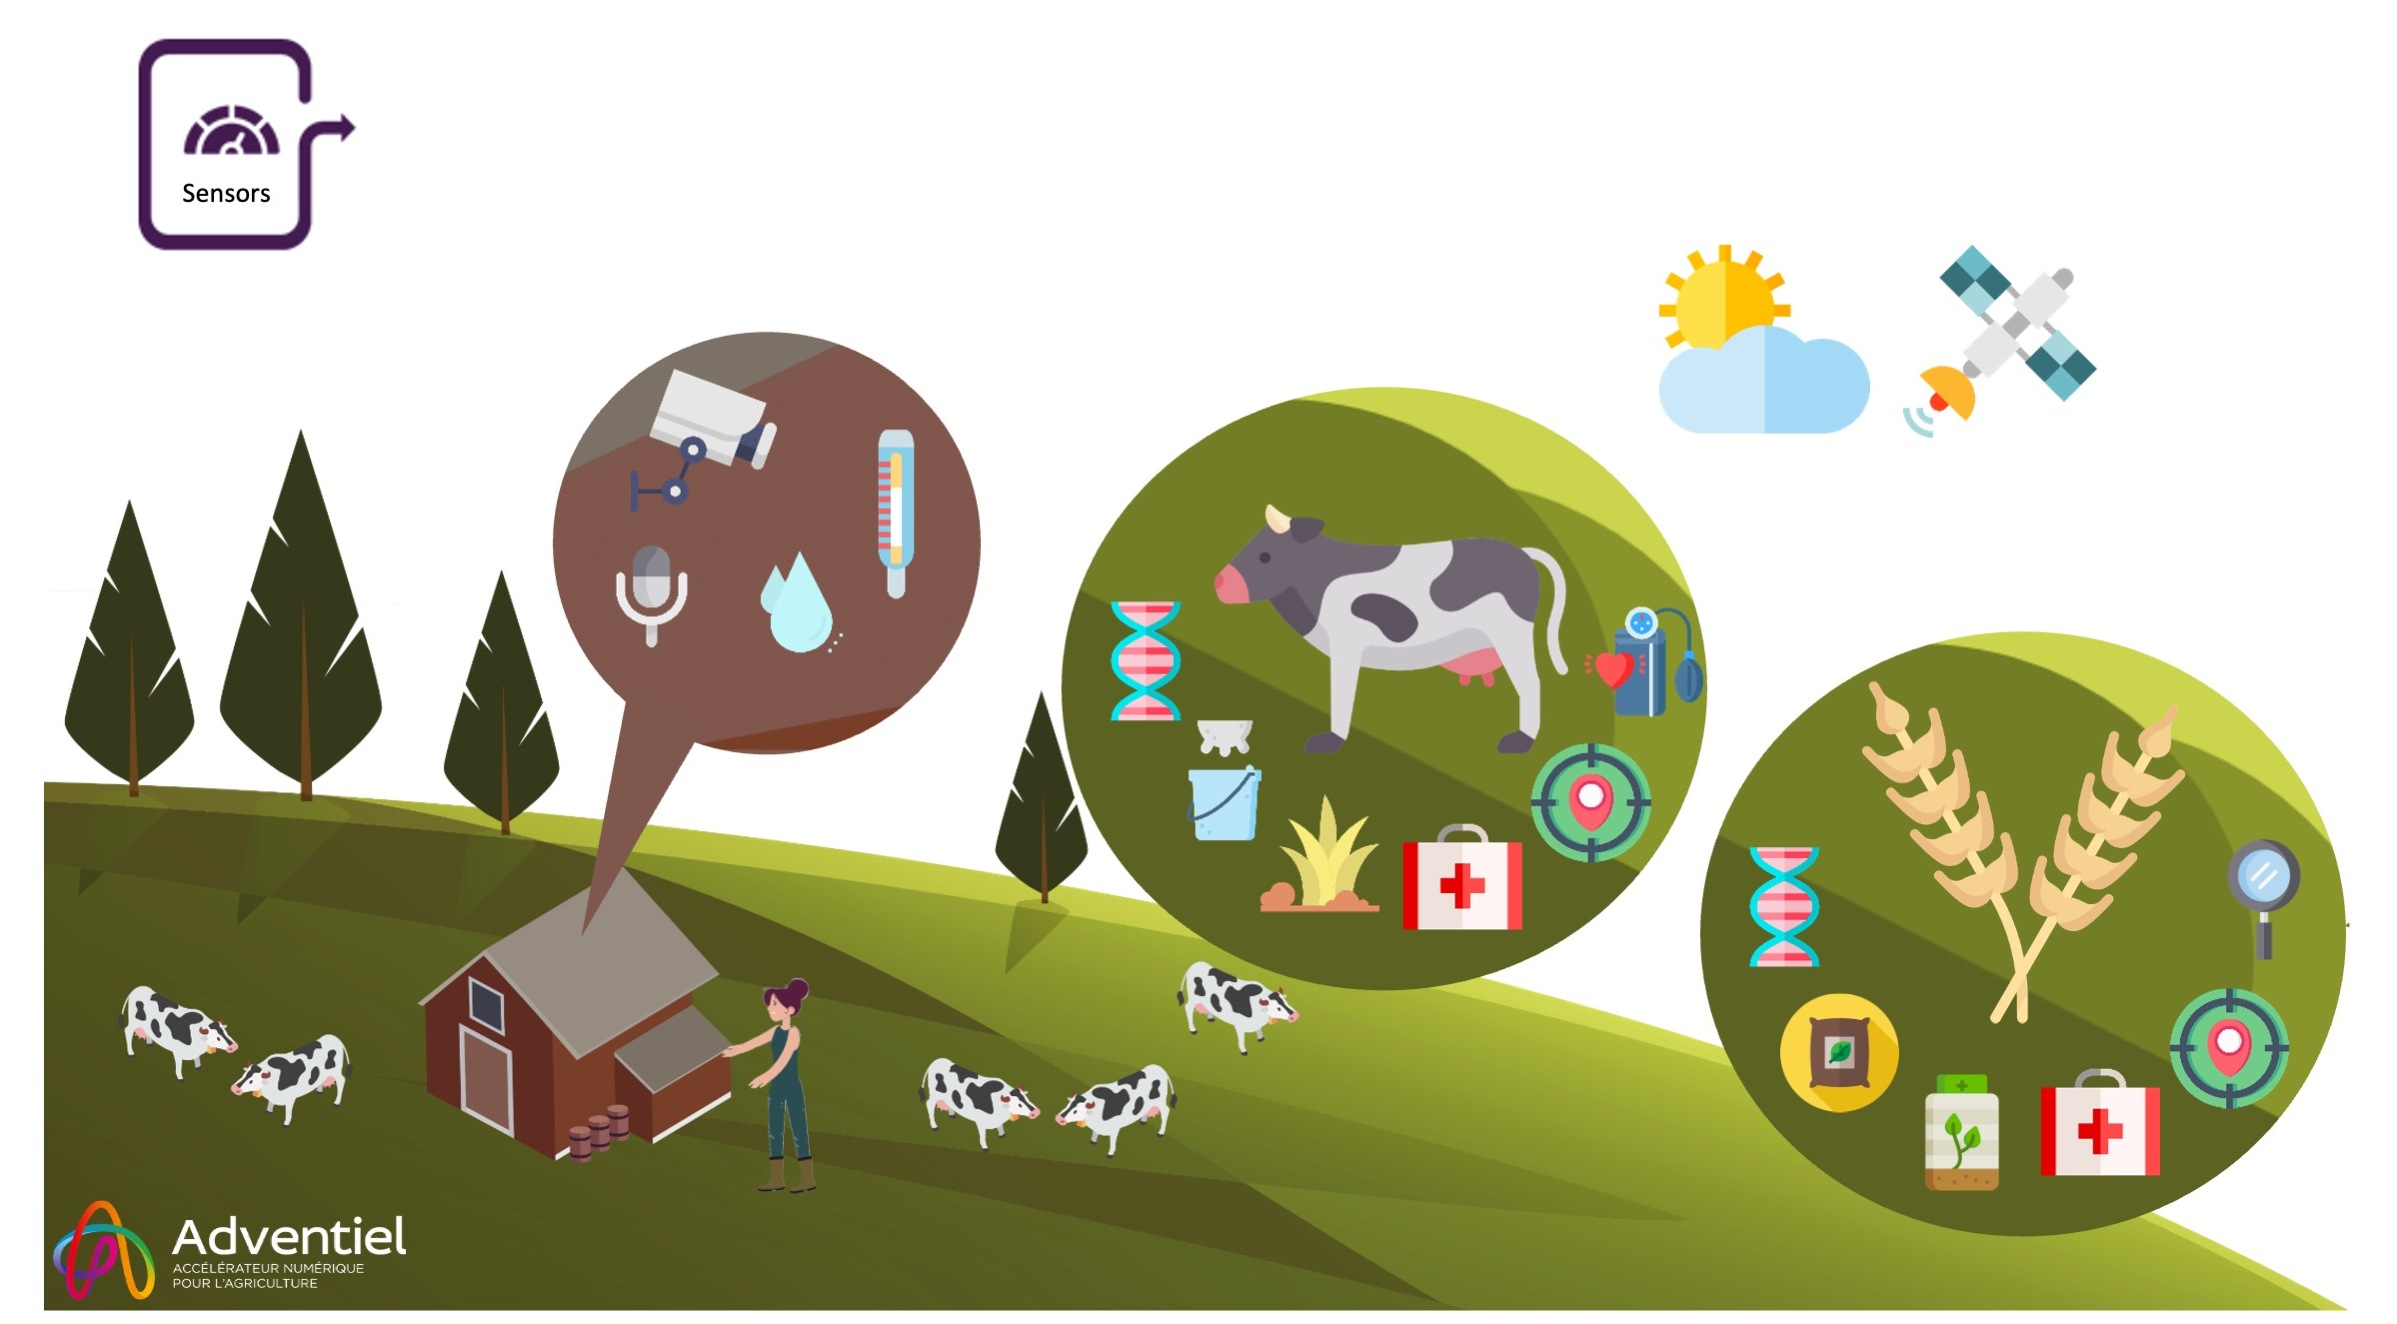
\includegraphics[width=\linewidth]{figures/chap1/chap1-sensors.jpg}
  \caption{Illustration of the diversere categories of observations that can be collected by sensor in livestock farming}
  \label{fig:chap1-sensors}
\end{figure}
\newpage

%%%%%%%%%

% Precision agriculture represents an innovative approach to farming that focuses on optimizing inputs (such as feed, medication, and energy) while maximizing outputs, including net profit and environmental sustainability. This paradigm is rapidly being adopted in livestock farming to enhance decision-making and operational efficiency. At its core, precision agriculture is supported by a robust infrastructure consisting of both hardware and software components. In this subsection, we concentrate on 



\subsection{Epidemiological modelling: Stochastic mechanistic models}

Mechanistic models in epidemiology have played a central role in translating complex, interdisciplinary insights into quantitative frameworks that inform evidence-based policy-making. Their construction begins by segmenting the population into compartments, typically susceptible, infected, and recovered, following seminal work by Bernoulli (1760), Ross (1916), and Kermack and McKendrick (1927) as detailed in early epidemiological studies. These foundational models not only formalized the understanding of disease transmission dynamics through systems of differential equations but also provided a platform for incorporating additional layers of biological, economic, and social theory into rule-based algorithms.

Building on these early models, researchers have developed increasingly sophisticated mechanistic models that integrate heterogeneous mixing patterns, demographic processes, and spatial structures. In the context of livestock infectious diseases, for instance, models have been extended to capture multi-scale interactions—from within-host processes to regional spread, thereby enabling the simulation of targeted interventions such as vaccination and movement restrictions 
\cite{Tomley2009, OIE2015}. The ability to embed theoretical insights into mathematical formulations allows these models to explore scenarios that are otherwise ethically or logistically infeasible to observe directly. This is crucial for policy-making, as it offers decision-makers evidence-based insights into the potential impacts of various control measures on both disease spread and animal welfare \cite{Ezanno2018, EZANNO2020100398}

The construction of these models generally involves formulating a set of differential equations or stochastic processes that describe transitions between defined compartments. Parameters such as the transmission rate, recovery rate, and contact structure are estimated using empirical data through methods like maximum likelihood estimation or Bayesian inference \cite{Keeling2008, Courcoul2010}. These fitting procedures are critical to ensure that the model outputs faithfully represent the underlying biological processes. However, a significant challenge arises from the increasing use of sensor-based data in modern epidemiological studies. Unstructured datasets, such as video and audio recordings from precision livestock farming, are rich in information yet notoriously difficult to process and integrate into these models due to the labour-intensive nature of manual data curation. The relevance of the model only depends on its use and the available data/knowledge to build and parametrize it. 

While preliminary efforts have begun to explore deep learning techniques for handling such unstructured data, the primary strength of mechanistic models lies in their capacity to consolidate interdisciplinary theoretical knowledge into a structured, predictive framework. This integration not only supports the evaluation of control strategies under diverse scenarios but also provides a safe, ethical alternative to field experimentation by simulating conditions that are hard to replicate in reality.


\subsection{Machine learning modelling: classical deep learning models}

Machine learning is an integral subfield of artificial intelligence that focuses on automatically deriving predictive models directly from datasets rather than embedding knowledge via mechanistic, rule‐based models such as those used in traditional epidemiology. In essence, it’s like teaching a child to recognize a cat by showing hundreds of pictures rather than providing explicit instructions \cite{rosenblatt1958perceptron}. At its core, deep learning creates multi-layered models that learn by adjusting their internal parameters based on examples. For instance, in image recognition, the first layers may detect simple features like edges and colours, while later layers combine these features to identify more complex patterns, such as the specific contours and textures that form a cat’s face \cite{Goodfellow-et-al-2016}. Early work in this area started with simple rule-based systems and perceptron models \cite{rosenblatt1958perceptron} and evolved over the decades into architectures that can span 10 to over 100 layers with tens to hundreds of millions of parameters \cite{Goodfellow-et-al-2016}. These deep models function as universal approximators, capable of modelling highly non-linear relationships by iteratively minimizing prediction error through back-propagation \cite{rumelhart1986learning} and stochastic gradient descent techniques that adjust millions of weights over thousands to millions of iterations using mini-batches of 32–512 samples \cite{hinton2012deep}. 

Among the classical deep learning models, several architectures have been particularly influential. Feed-forward neural networks serve as the basic building blocks in which data flows in one direction from input to output. Convolutional neural networks  have revolutionized computer vision by applying convolutional filters and max pooling operations to extract spatial hierarchies from high-resolution images (often 512×512 pixels or larger) and achieve translational invariance \cite{lecun1998gradient, krizhevsky2012imagenet}. Recurrent neural networks , and particularly their long short-term memory  variants, are engineered to handle sequential data by overcoming issues like the vanishing gradient problem through gating mechanisms, thus capturing dependencies that span thousands of time steps 
\cite{hochreiter1997long, graves2005framewise}. More recently, graph neural networks have emerged to model data with non-Euclidean structures—such as relationships in social networks or complex interactions on a farm \cite{scarselli2009graph}, while transformer models leverage self-attention mechanisms to process entire sequences in parallel, which improves the modelling of long-range dependencies and reduces training time \cite{vaswani2017attention}. In addition to these traditional architectures, foundational models—particularly large language models such as GPT (generative pre-trained transformer) have revolutionized natural language processing by being trained on vast amounts of text data to predict and generate human-like language \cite{brown2020language}. However, a significant challenge for these models is “hallucination,” where they generate plausible-sounding but factually incorrect or nonsensical outputs. This occurs because these models rely on statistical patterns rather than deep, mechanistic understanding, lacking strong theoretical grounding in the underlying principles of language \cite{marcus2020gpt3, bender2021stochastic}. In contexts like livestock management, where deep learning applications in natural language processing are used to analyse veterinary reports and sensor logs, such hallucinations can lead to false positive and incorrect diagnoses or misguided recommendations, highlighting the need for integrating explicit domain knowledge to improve reliability \cite{smith2020nlp}.

Because these deep learning models can have millions of parameters and many layers, they are often described as "black boxes" systems that deliver high accuracy yet offer little insight into how decisions are made. This opacity is problematic, especially in high-stakes domains such as healthcare, autonomous driving, or livestock management, where understanding a model’s rationale is crucial for safety and trust \cite{bengio2013representation}. Explainable Artificial Intelligence (XAI) addresses this gap by providing methods to interpret and understand the internal workings of complex models. For example, Gradient-weighted Class Activation Mapping (Grad-CAM) generates visual maps that indicate which parts of an image were most influential for the model’s decision, and Local Interpretable Model-agnostic Explanations (LIME) approximate a deep model’s local behaviour with a simpler, interpretable model for specific instances 
\cite{ribeiro2016should, selvaraju2017grad}. Another critical component is uncertainty quantification, which ensures that a model not only provides a prediction but also a measure of confidence in that prediction. Bayesian Neural Networks use variational methods to assign probability distributions to model parameters, so instead of providing a single fixed output, the network indicates, for example, that it is 90\% confident that an image contains a cat, with the remaining 10\% reflecting uncertainty \cite{gal_dropout_2016}. Similarly, conformal prediction techniques provide statistically valid prediction sets, ensuring that the true outcome is contained within these sets at a pre-defined confidence level \cite{Angelopoulos2021}.

Transformer-based models have been deployed to automatically analyse veterinary clinical records, social media posts from farmers, and sensor-generated text logs to identify early signs of disease outbreaks or stress in livestock populations \cite{smith2020nlp}. Deep learning models have also been used to monitor animal behaviour through video analysis, allowing for the  detection of anomalies such as lameness or aggressive behaviour, thereby enabling timely interventions that improve animal welfare and productivity 
\cite{fischer2018deep, kamphuis2017animal}. Other studies have demonstrated the utility of deep learning in livestock management by combining image analysis with sensor data. For example, CNNs have been used to automatically count and classify animals in large herds, while natural language processing helps in summarizing and integrating textual data from various reports, creating a comprehensive monitoring system that can alert farmers to potential issues before they escalate \cite{raboisson2017machine, bakker2019predictive, lopez2020integrated}.

All these techniques, deep neural architectures and its security techniques such as XAI methods and uncertainty quantification tools, come together to form a more robust and transparent system. By explaining their inner workings and providing confidence measures, these methods help users understand not only what the model’s decision is, but also why it made that decision and how reliable that decision is. This comprehensive approach is especially important in fields where decisions have significant consequences, such as in medical diagnosis, financial forecasting, or autonomous driving \cite{hinton2012deep, bengio2013representation}. Without integrating additional domain-specific knowledge, these models can struggle to generalize beyond the data on which they were trained, leaving significant opportunities for further research at the intersection of deep learning and mechanistic modelling. 


\subsection{Hybrid modelling: machine learning and epidemiological models}

Recent research in infectious disease modelling has sought to address the well‐known limitations of data‐driven and theoretical approaches when used in isolation. Deep learning methods, while highly effective at capturing complex, non-linear patterns from structured data, often struggle to extrapolate when confronted with untrained or sparse data. In contrast, mechanistic epidemiological models, which are built upon established theoretical principles of disease dynamics, frequently face challenges when fitting unstructured observations. This has led to the development of several hybrid integration approaches that aim to merge the complementary strengths of both methodologies to achieve objectives such as forecasting, model parametrization and calibration, intervention assessment and optimization, retrospective epidemic course analysis, transmission inference, and outbreak detection \cite{Ye2025}.

One prominent integration approach involves using Physics-Informed Neural Networks (PINNs) and Epidemiology-Augmented Artificial Models (EAAMs) to learn unknown components of epidemiological models. In these methods, deep learning architectures are augmented by incorporating epidemiological principles directly into the network—often through residual loss terms—to learn hidden state variables, parameters, or derivatives. This approach helps model parametrization and calibration while also improving forecasting capabilities by enforcing consistency with known epidemic dynamics. Studies employing this method have demonstrated its effectiveness on both real and synthetic datasets, as documented in recent literature \cite{kharazmi_identifiability_2021, barmparis_physicsinformed_2022, de_rosa_modelling_2023, torku_seinn_2023,berkhahn_physics-informed_2022, rodriguez_einns_2023, shaier_data-driven_2022, bertaglia_asymptotic-preserving_2022, malinzi_determining_2022} for PINNs; \cite{liu_rolling_2023, otadi_universal_2017, liu_epidemiology-aware_2023, amini_mepognn_2023, sun_2022, gao_stan_2021, zheng_spatial-temporal_2021, ma_enhancing_2022, wang_causalgnn_2022, nguyen_becaked_2022, nguyen_becaked_2022-1} for EAAMs 

% and \cite{wang_tdefsi_2020, zhan_optimizing_2021, wang_deep_2021, bogacsovics_replacing_2021, wang_predicting_2022, murphy_deep_2021, zhang_understanding_2021, quilodran-casas_digital_2022, silva_data_2022}
%[69–77, 78–88].

Another strategy leverages mechanistic models to generate synthetic datasets under varied parameter conditions. Deep learning architectures, such as recurrent neural networks, are then trained on these synthetic datasets to predict unobserved model components or forecast future epidemic trajectories. By doing so, this approach addresses the challenge of limited real-world data and contributes significantly to both forecasting and transmission inference. The synthetic data enable the model to generalize beyond the training domain, thereby enhancing its capacity to infer underlying transmission patterns in scenarios where observational data are sparse \cite{petrica_inverse_2023,liu_prediction_2023,rahnsch_network-based_2024,kumar_epidemic_2023,ji_climate-dependent_2023,vega_simlr_2022,chen_covid-19_2023,alsmadi_susceptible_2023,qiu_prediction_2022,mu_modelling_2023,wang_machine_2021,wu_computer_2022,yao_assessment_2022,zhang_prediction_2021,wyss_modeling_2023,gadewadikar_methodology_2024,zisad_integrated_2021,merkelbach_hybridml_2022,munoz_hybrid_2022,castillo_ossa_hybrid_2021,jiang_countrywide_2021,yasami_application_2022,liao_sirvd-dl_2021,zheng_predicting_2020,watson_pandemic_2021,liu_nesting_2023,wang_policy_2022,wang_hypothesis-free_2022,deng_dynamics_2020,kim_determination_2021,gupta_deep-siqrv_2023,bousquet_deep_2022,feng_data_2022,ding_biology-informed_2023,khan_attention_2022,kumaresan_analysis_2022,long_identification_2021}

A further integration approach embeds epidemiological constraints directly within deep learning frameworks. By incorporating established conservation laws or differential equations into the model’s inputs, loss functions, or architecture, these hybrid models ensure that predictions adhere to the theoretical underpinnings of disease dynamics. This method improves both the accuracy of forecasts and the robustness of retrospective epidemic course analyses by aligning data-driven predictions with fundamental epidemiological knowledge \cite{kharazmi_identifiability_2021,barmparis_physicsinformed_2022,de_rosa_modelling_2023,torku_seinn_2023,berkhahn_physics-informed_2022,rodriguez_einns_2023,shaier_data-driven_2022,bertaglia_asymptotic-preserving_2022,malinzi_determining_2022}. In a related vein, reinforcement learning and optimal control frameworks have been integrated into simulation environments derived from mechanistic models. In these approaches, reinforcement learning agents interact with epidemiologically informed simulations to iteratively optimize intervention strategies. This methodology directly addresses the objective of disease intervention assessment and optimization by enabling the exploration of optimal control policies through continuous feedback from the simulation environment \cite{yao_optimal_2023,zou_data-efficient_2021,vereshchaka_optimization_2021,song_reinforced_2020,probert_context_2019,ohi_exploring_2020,khadilkar_optimising_2020,hao_reinforcement_2022,libin_deep_2021,awasthi_vacsim_2022,song_robust_2023,padmanabhan_reinforcement_2021,kompella_reinforcement_2020,mai_planning_2023,asikis_neural_2022,roy_knowledge_2021,colas_epidemioptim_2021,capobianco_agent-based_2021,ou_active_2021,trad_towards_2022,bushaj_simulation-deep_2022,chadi_2022 ,guo_pacar_2022,kulkarni_optimizing_2022,deng_optimal_2021,hwang_optimal_2022,wan_multi-objective_2022,miralles-pechuan_methodology_2020,bampa_epidrlearn_2022,shami_economic_2022,du_district-coupled_2022,benalcazar_deep_2021,xia_controlling_2022,khatami_reinforcement_2021,zong_reinforcement_2022,du_hrl4ec_2023,nguyen_general_2022,beigi_application_2021} for RL methods and \cite{yin_optimal_2023,asikis_neural_2022,courtes_reduced_2024,li_robust_2021,kmet_neural_2023,kmet_bezier_2019} for optimal control frameworks.

Additional integration strategies focus on enhancing the quality of unstructured observational data and reducing prediction error. Techniques such as support vector machines and tree-based classifiers are applied to extract auxiliary information from heterogeneous datasets, thereby refining parameter estimation and indirectly supporting retrospective analysis and outbreak detection. Moreover, ensemble modelling methods, which combine outputs from independently trained models through stacking, boosting, or bagging, have been shown to reduce overall prediction error and increase robustness. These ensemble techniques facilitate improved forecasting accuracy and more reliable outbreak detection by synthesizing diverse model predictions \cite{tuarob_modeling_2015,solares-hernandez_adaptation_2023,rosato_extracting_2023,kandula_improved_2019} and 
\cite{kandula_evaluation_2018,adiga_all_2021,nadler_neural_2020,maniamfu_lstm-based_2023,adiga_enhancing_2022,delli_compagni_hybrid_2022}. Complementing these methods, Bayesian neural networks have been employed to quantify uncertainty in parameter inference. By approximating the posterior distribution of model parameters, this approach provides critical measures of confidence that enhance forecasting, transmission inference, and outbreak detection \cite{ryder2018blackboxvariationalinferencestochastic, ARNST2022108805, 10.1371/journal.pcbi.1005416, 10.1371/journal.pcbi.1009472}. Finally, clustering-based decomposition uses unsupervised learning algorithms, such as k-means, to partition large-scale epidemiological models into smaller sub-models. This segmentation enables localized analysis and tailored intervention strategies, thereby strengthening retrospective epidemic course analysis and improving the sensitivity of outbreak detection \cite{bertozzi-villa_archetypes_2023}.

Among the studies reviewed, a total of 26 infectious diseases were investigated using integrated models. Notably, COVID-19 dominated the research landscape, accounting for 60\% of the studies, with 148 investigations dedicated to this disease. Influenza was the focus in 7\% of the studies, dengue in 2\%, and HIV in 1\%. In addition, 23\% of the studies utilised hypothetical disease scenarios to demonstrate the applicability of the methods. Based on the reviewed studies, there isn’t strong evidence that sensor observations—such as data directly collected from IoT devices or on‐farm sensors—have been prominently integrated into these frameworks. Some work has explored the use of sensor‐based data like satellite imagery (which is one form of sensor observation) to capture environmental factors. However, most approaches in the review primarily rely on traditional surveillance data and non‑traditional sources such as social media, search queries, or emergency reports, rather than sensor observations from livestock or similar settings. This represents an opportunity for future research to incorporate direct sensor data for automated monitoring and relevant context-specific insights.


%%%%%%%%%
% This section serves as a concise narrative review of various methodologies for integrating machine learning models with epidemiological models, offering a critical perspective on their limitations. Addressing these limitations is central to the contributions of this thesis.

% This section presumes that the reader possesses a foundational understanding of ensemble techniques in modelling, specifically bagging, boosting, and stacking. They are pivotal in enhancing the global performance by combining multiple models. These methods aim to reduce errors, improve accuracy, and increase the robustness of predictions. Stacking Combines outputs from several distinct models using an additional "meta-model," learning optimal combinations for improved predictions. Boosting refers to sequentially training multiple weak predictive models, each aiming to correct errors from previous models, thus progressively improving overall prediction accuracy. Bagging (or Bootstrap Aggregating) refers to parallel training of multiple unique models (while stacking used distinct models, bagging uses multiple instances but of the same model) on random subsets of data (with replacement), thereby reducing prediction variance and mitigating over-fitting.



% En sciences, toute tentative de tirer des conclusions généralisables nécessite un
% modèle, i.e. une version abstraite de la réalité \cite{McCallum2008}. Cette représentation
% abstraite est dotée d’un objectif (a model is a "purposeful representation", 
% \cite{Starfield1990}, qui requiert un certain degré de simplification.




% Methodologicaly-wise, these models can also grouped into nine primary integration approach. Figure \ref{fig:chap1-hybrid} illustrates several methodological frameworks that integrate machine learning with mechanistic epidemiological models.  In the first integration method—Learning Unknown Components of Epidemiological Models, AI models (namely PINNs, EAAMs, and synthetically-trained AI models) are employed to “learn” the unknown elements of mechanistic models, such as state variables, parameters, or derivatives. The integration is achieved by incorporating epidemiological principles,often in the form of residual loss terms—directly into the network architecture, as shown in figure \ref{fig:chap1-hybrid} (subplot c) The training process consists of end-to-end supervised training using gradient-based optimization (e.g., Adam or SGD) applied on real or synthetic datasets. The original citations for this method are \cite{kharazmi_identifiability_2021, barmparis_physicsinformed_2022, de_rosa_modelling_2023, torku_seinn_2023,berkhahn_physics-informed_2022, rodriguez_einns_2023, shaier_data-driven_2022, bertaglia_asymptotic-preserving_2022, malinzi_determining_2022} for PINNs; \cite{liu_rolling_2023, otadi_universal_2017, liu_epidemiology-aware_2023, amini_mepognn_2023, sun_2022, gao_stan_2021, zheng_spatial-temporal_2021, ma_enhancing_2022, wang_causalgnn_2022, nguyen_becaked_2022, nguyen_becaked_2022-1} for EAAMs; and \cite{wang_tdefsi_2020, zhan_optimizing_2021, wang_deep_2021, bogacsovics_replacing_2021, wang_predicting_2022, murphy_deep_2021, zhang_understanding_2021, quilodran-casas_digital_2022, silva_data_2022}.

% The second method—Training AI Models Using Synthetic Data (Fig \ref{fig:chap1-hybrid} subplot e), uses mechanistic models to generate synthetic datasets under varying parameter conditions. In this approach, AI models such as recurrent neural networks (RNNs) are trained on these synthetic datasets with the aim of predicting unknown model components or future epidemic trajectories. The training is performed using standard supervised learning methods on synthetic data. The corresponding citations for this method are \cite{petrica_inverse_2023,liu_prediction_2023,rahnsch_network-based_2024,kumar_epidemic_2023,ji_climate-dependent_2023,vega_simlr_2022,chen_covid-19_2023,alsmadi_susceptible_2023,qiu_prediction_2022,mu_modelling_2023,wang_machine_2021,wu_computer_2022,yao_assessment_2022,zhang_prediction_2021,wyss_modeling_2023,gadewadikar_methodology_2024,zisad_integrated_2021,merkelbach_hybridml_2022,munoz_hybrid_2022,castillo_ossa_hybrid_2021,jiang_countrywide_2021,yasami_application_2022,liao_sirvd-dl_2021,zheng_predicting_2020,watson_pandemic_2021,liu_nesting_2023,wang_policy_2022,wang_hypothesis-free_2022,deng_dynamics_2020,kim_determination_2021,gupta_deep-siqrv_2023,bousquet_deep_2022,feng_data_2022,ding_biology-informed_2023,khan_attention_2022,kumaresan_analysis_2022,long_identification_2021} .

% Another approach embeds epidemiological knowledge directly into AI models. In this method, known epidemiological constraints, such as conservation laws or differential equations that govern disease spread—are integrated into the AI model’s inputs, loss functions, or architecture. The objective is to enforce that the predictions adhere to established epidemic dynamics. This method typically uses gradient-based supervised training on real datasets, although synthetic data may also be incorporated. (Fig \ref{fig:chap1-hybrid} subplot a \& d) outlines the architecture where epidemiological inputs and custom loss functions work together to constrain the learning process. The studies related to this method are detailed in the related references \cite{kharazmi_identifiability_2021,barmparis_physicsinformed_2022,de_rosa_modelling_2023,torku_seinn_2023,berkhahn_physics-informed_2022,rodriguez_einns_2023,shaier_data-driven_2022,bertaglia_asymptotic-preserving_2022,malinzi_determining_2022}.

% The next method focuses on optimal decision-making through AI models, particularly using reinforcement learning (RL) or optimal control frameworks. In these approaches, mechanistic models provide simulated environments where RL agents learn optimal intervention strategies through iterative interactions. The training process involves training RL agents within epidemiologically based environments or using neural networks to approximate control variables through iterative optimization techniques. The method has been applied to assess intervention policies in settings like the COVID-19 pandemic. (Fig \ref{fig:chap1-hybrid} subplot h) displays the interaction between the RL agent and the simulation environment, highlighting the iterative nature of the learning process. The original citations for this method are \cite{yao_optimal_2023,zou_data-efficient_2021,vereshchaka_optimization_2021,song_reinforced_2020,probert_context_2019,ohi_exploring_2020,khadilkar_optimising_2020,hao_reinforcement_2022,libin_deep_2021,awasthi_vacsim_2022,song_robust_2023,padmanabhan_reinforcement_2021,kompella_reinforcement_2020,mai_planning_2023,asikis_neural_2022,roy_knowledge_2021,colas_epidemioptim_2021,capobianco_agent-based_2021,ou_active_2021,trad_towards_2022,bushaj_simulation-deep_2022,chadi_2022 ,guo_pacar_2022,kulkarni_optimizing_2022,deng_optimal_2021,hwang_optimal_2022,wan_multi-objective_2022,miralles-pechuan_methodology_2020,bampa_epidrlearn_2022,shami_economic_2022,du_district-coupled_2022,benalcazar_deep_2021,xia_controlling_2022,khatami_reinforcement_2021,zong_reinforcement_2022,du_hrl4ec_2023,nguyen_general_2022,beigi_application_2021} for RL methods and \cite{yin_optimal_2023,asikis_neural_2022,courtes_reduced_2024,li_robust_2021,kmet_neural_2023,kmet_bezier_2019} for optimal control frameworks.

% Enhancing observational data constitutes another integration strategy. Here, AI techniques—using methods such as support vector machines or tree-based classifiers, are employed to extract auxiliary information (infer health status and generate enhanced observational datasets) from non-traditional data sources (e.g., text from social media, emergency reports) and improve the quality of conventional epidemiological datasets. This method, which generally relies on real data, refines model parameter estimation. (Fig \ref{fig:chap1-hybrid} subplot b) illustrates how enhanced data inputs feed into the epidemiological model to improve its performance. The original citations for this method are \cite{tuarob_modeling_2015,solares-hernandez_adaptation_2023,rosato_extracting_2023,kandula_improved_2019}.

% Ensemble modelling of AI and epidemiological models is yet another integration approach where outputs from distinct models are combined using techniques like weighted averaging, stacking, or boosting, to improve forecasting accuracy.  In this framework, individual models are first trained separately on either real or synthetic data; subsequently, a meta-model (for instance, an LSTM-based stacker) is trained on historical performance to combine these outputs into a final forecast. The original citations for this approach are \cite{kandula_evaluation_2018,adiga_all_2021,nadler_neural_2020,maniamfu_lstm-based_2023,adiga_enhancing_2022,delli_compagni_hybrid_2022}. This approach has been applied, for instance, in COVID-19 forecasting, and (Fig \ref{fig:chap1-hybrid} subplot f)depicts the ensemble process with multiple model outputs converging into a final prediction.

% One approach employs Bayesian neural networks to enhance parameter inference within mechanistic epidemiological models. In this framework, the neural network is structured to quantify uncertainty by approximating the posterior distribution of model parameters, a critical capability when dealing with intractable likelihoods or limited data. The training process typically involves optimizing variational objectives, such as maximizing the evidence lower bound (ELBO), using real-world observational datasets. (Fig \ref{fig:chap1-hybrid} subplot g) illustrates the architecture that integrates uncertainty quantification directly into the model. The original studies detailing this approach are referenced in \cite{ryder2018blackboxvariationalinferencestochastic, ARNST2022108805, 10.1371/journal.pcbi.1005416, 10.1371/journal.pcbi.1009472}.

% Lastly, clustering-based decomposition of epidemiological models (Fig \ref{fig:chap1-hybrid} subplot i) offers a means to break down large-scale, complex models into smaller, more manageable sub-models. By applying clustering algorithms (such as k-means) to group regions or populations with similar epidemic characteristics, this approach allows for localized analysis and tailored intervention strategies. Typically leveraging unsupervised learning, these methods primarily work with real-world data but can also incorporate synthetic data in simulation studies. They are particularly useful for targeted outbreak detection and evaluation of region-specific intervention impacts \cite{bertozzi-villa_archetypes_2023} . Figure 1.1 provides a schematic of how clustering methods break down the overall model into manageable sub-models.

% \begin{itemize}
%     \item Physics-Informed Neural Networks (PINNs): PINNs integrate known governing equations (e.g., differential equations describing infectious dynamics) as soft constraints into neural networks during training. The neural network is guided by both observed data and theoretical knowledge, ensuring physically plausible predictions and improved extrapolation beyond the training distribution.
%     \item Neural Differential Equations (Neural ODEs/SDEs): Neural ODEs or SDEs embed neural networks into differential equations, allowing the modelling of dynamic processes through continuous-time representations. Such integration directly captures temporal dynamics, offering more flexibility and interpretability compared to classical discrete-time deep learning methods.
% \end{itemize}

% Despite their promising advantages, hybrid and ensemble models have inherent challenges:
% Despite notable advancement in the scientific community, there is a conceptual gap, between the raw unstructured livestock data that can be captured and the strong theoretical knowledge we have of the complex underlying infectious mechanisms. This basically allows to ground the theoretical knowledge we have on a complex mechanisms to the context-specific observations, hence harness the best of both world. 

% \begin{figure}[h]
%   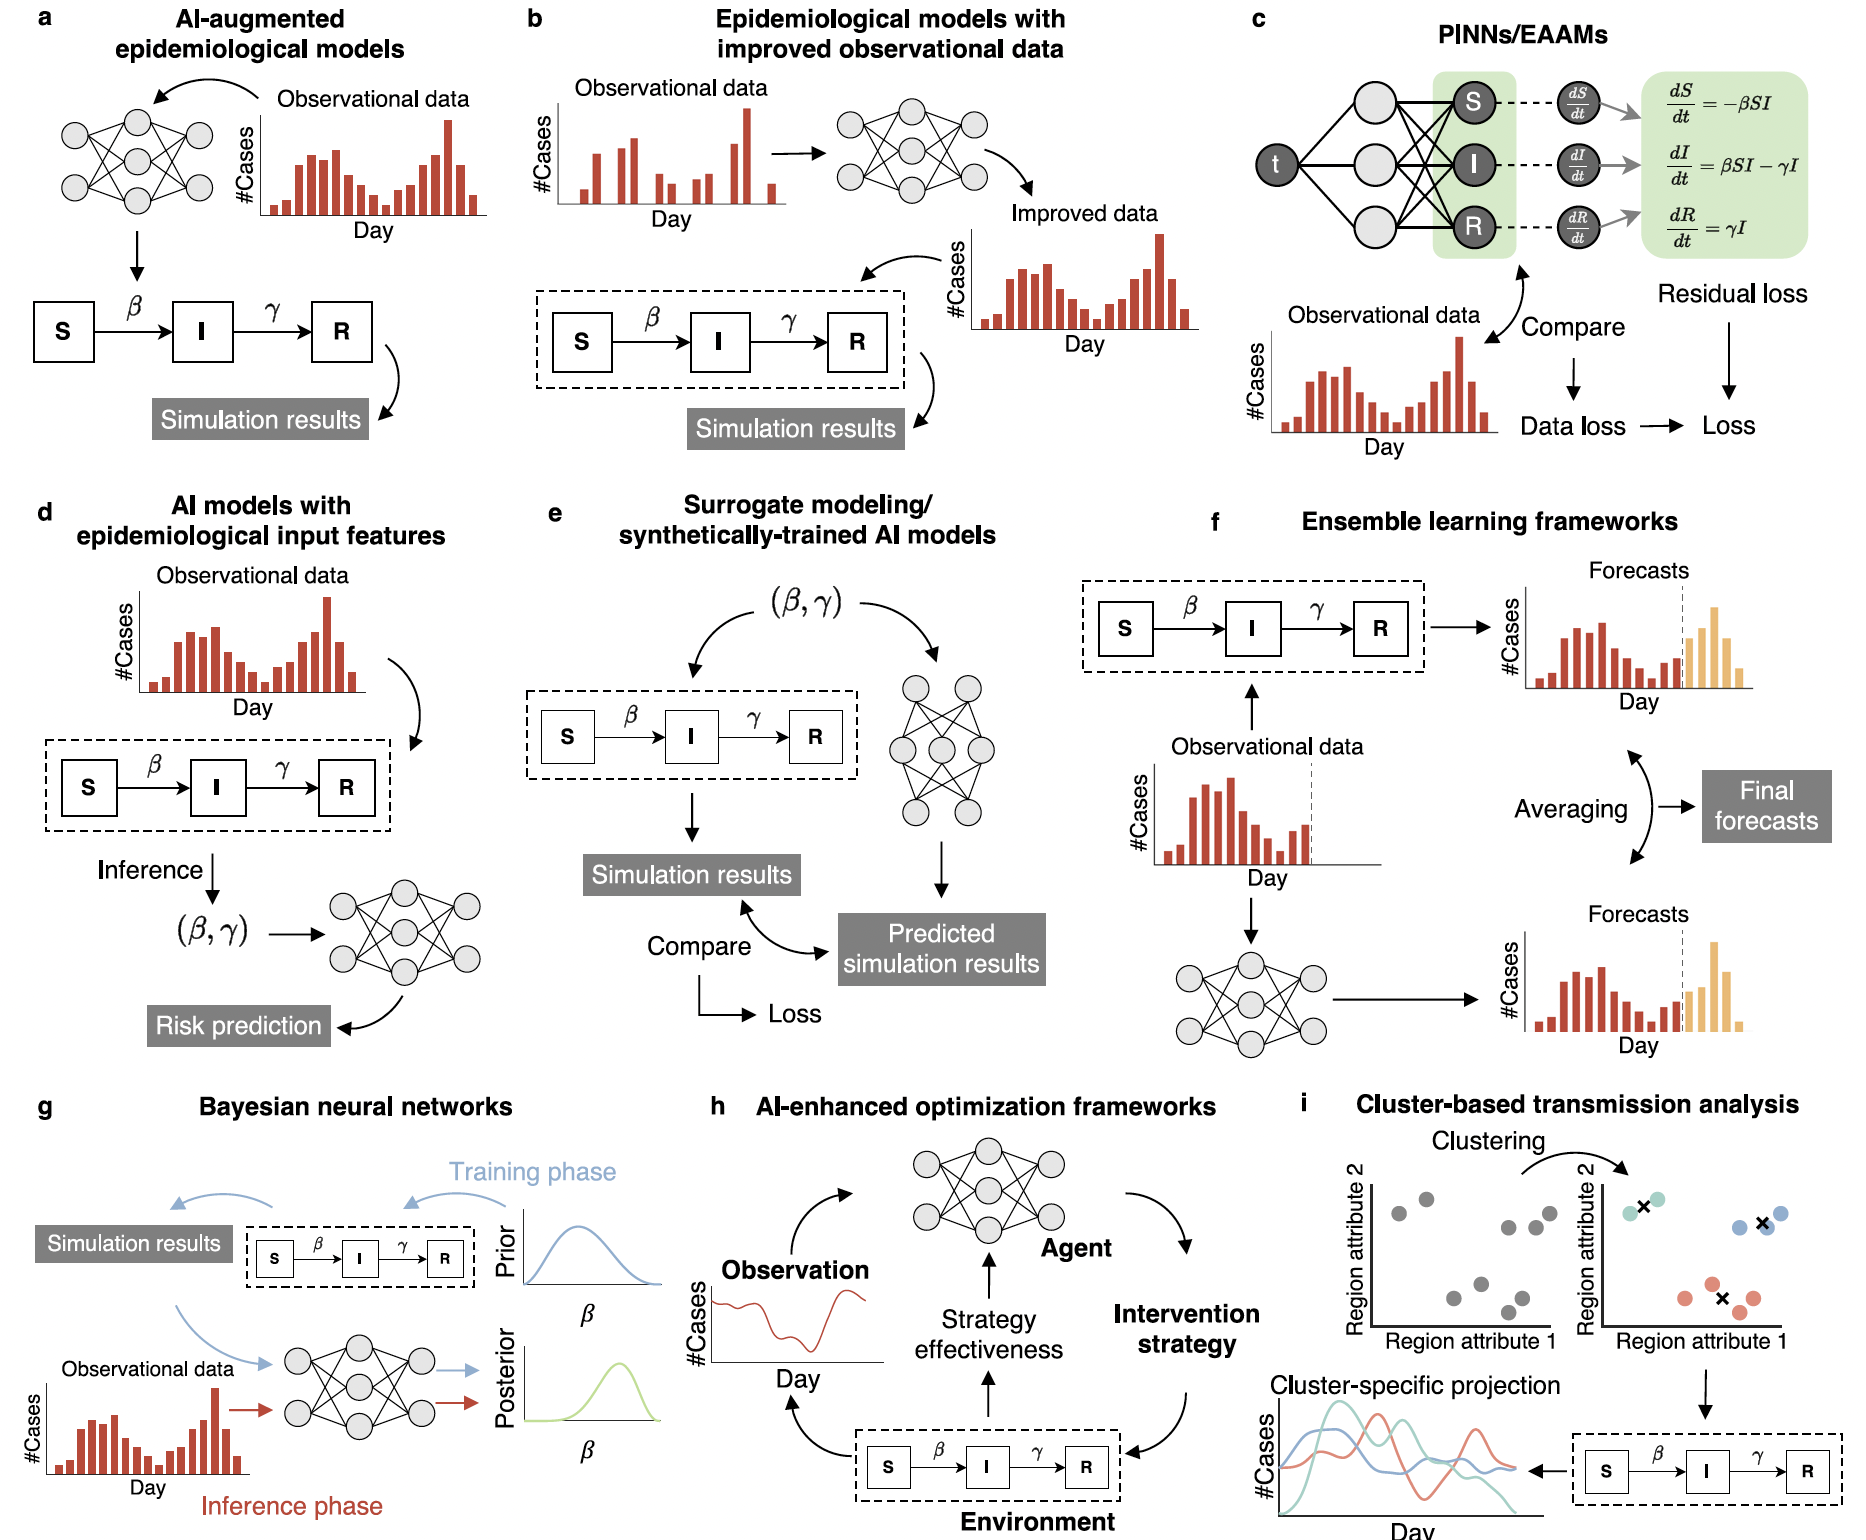
\includegraphics[width=\linewidth]{figures/chap1/chap1-hybrid.png}
%   \caption{Illustrative examples of methodological frameworks coupling Machine learning and epidemiological models}
%   \label{fig:chap1-hybrid}
% \end{figure}


% Among the studies reviewed, a total of 26 infectious diseases were investigated using integrated models. Notably, COVID-19 dominated the research landscape, accounting for 60\% of the studies, with 148 investigations dedicated to this disease. Influenza was the focus in 7\% of the studies, dengue in 2\%, and HIV in 1\%. In addition, 23\% of the studies utilized hypothetical disease scenarios to demonstrate the applicability of the methods, rather than concentrating on a specific infectious disease. These are studies that are the closest to the question this thesis is trying to bring a part of answer to.


% Each ensemble strategy presents specific strengths and limitations, related to computational complexity, interpretability, and predictive power. 
% research gaps:
% \begin{itemize}
%     \item Generalizability: The majority of integrated models focus on diseases like COVID-19, limiting applicability to other infectious diseases with indirect or complex transmission routes.
%     \item Expansion beyond COVID-19 to other diseases with indirect transmission mechanisms.
%     \item Data Limitations: Many studies depend on synthetic or limited real-world data, highlighting the need for richer, real-time data integration (e.g., satellite imagery, social media data). - we have gathered in this thesis a real-wolrd multi-modal dataset (...)
% \end{itemize}

% je vais enlever cette subsub section, elle ne sert à rien
% \subsubsection*{Maintainability}

%     \begin{itemize}
%         \item strongly coupled methods requires the builder to be deeply understand the problematic of domain in order to implement the models. (full stack vs frontend or backend). So retraining for example would require the whole system to be trained and in the long-term, it would also require sort of full-stack builders. 
        
%         \item strongly coupled methods would still require a  certain quantity of data since in order for example for the deep learning model to fine-tune the mechanistic model (neural differential equations). Usually ensembled model (so more parameters) would require more dimensions in order to fit all the parameters (curse of dimensionality)
%     \end{itemize}

% le domaine est très large, mais nous on va se focaliser uniquement sur le couplage deep et modèle méchaniste de façon générale. 

% sachant que nous c'est une forme de boosting, sans trop de redondances,) et surtout découplé (faiblement couplé) - ceci sont des couplages forts mais comme un site web à egalement ces limites. comme un développeur full stack - parler rapidement des NDE, des pinns qui sont juste une sous familles des NDE.



%----------------------------------------------------------------------------------------
%	SECTION 
%----------------------------------------------------------------------------------------
\clearpage 

\section{Thesis objective and outline}

\subsection{Exploring the complementarities between deep learning and mechanistic epidemiological models}

Precision agriculture provides powerful tools enabling automation of real-world observations through various sensors. Throughout this thesis, we have leveraged such tools to acquire contextual observational data essential for studying an infectious disease in livestock farming. However, sensor-based observations, although rich and increasingly accessible, represent only partial information regarding complex and unpredictable disease dynamics, aptly summarized by Yoan Bourhis (2017): "Nos observations ne révèlent que la partie émergée d’un iceberg au comportement complexe et peu prévisible."

Thus, a central question guiding this thesis is: How can sensor observations be effectively employed to study infectious diseases and support informed decision-making?

Our main hypothesis is that the most scientifically robust approach to contemporary quantitative questions in animal health, particularly regarding livestock infectious diseases, lies in combining complementary artificial intelligence methods, specifically deep learning and mechanistic epidemiological models. Such integration leverages deep learning’s capabilities for processing and extracting short-term insights from unstructured (video, image or text) observations  and the extrapolative capacities of stochastic epidemiological models grounded in explicit theoretical knowledge for long-term insights. This combination aims to better link real-world observations obtained through sensors with our theoretical knowledge in order make make relevant evidence-based recommendations at a larger temporal scales.

This naturally raises another foundational question addressed in this thesis:
In what ways can deep learning complement mechanistic epidemiological models in epidemiology ?

Complex animal health problems, including the study and control of infectious diseases, require distinct yet interconnected types of expertise: diagnosing diseases from immediate observational data, making reliable prognoses about future disease dynamics, and ultimately providing actionable recommendations. Diagnosis relies predominantly on processing unstructured field observations from sensors—thus favouring deep learning. Robust prognosis, however, relies on explicit theoretical knowledge and interpretability—domains inherently suited to mechanistic models. Finally, the quality of actionable recommendations is critically dependent on effectively bridging these two forms of expertise.

This thesis proposes a loosely coupled methodology inspired by the statistical principle known as the "Mixture of Experts" (MoE). This modular integration allows each expert to specialize explicitly in its distinct role (diagnosis and prognosis), enhancing accuracy, resource efficiency, interpretability, and scalability.

Addressing these considerations, the scientific questions explored throughout this thesis are:

\begin{enumerate}
    \item To what extent can deep learning reliably automate short-term diagnosis using limited, noisy, and context-specific observational data from sensors, such as lung ultrasounds ? 
    
    \item How can mechanistic epidemiological models be reliably parametrized using empirical veterinary observations to provide accurate long-term prognosis for infectious diseases ?
    
    % \item Given multiple mechanistic epidemiological models validly representing different expertise symptomatic dynamics of infectious diseases, how can observational data alone reliably guide the selection of the most appropriate mechanistic model to enable pathogen-specific disease management ?
    
    % \item How can observational data alone guide the selection of the best mechanistic prognosis expert when they are multiple epidemiological models expert for expliciting different mechanisms of the infectious disease.
    
    \item Given multiple mechanistic epidemiological models representing different but valid expertise in prognosing an outbreak, how can observational data alone reliably guide the selection of the most appropriate mechanistic model to enable pathogen-specific disease management.

    \item How can deep learning and mechanistic models be effectively integrated into a hybrid diagnostic-to-prognostic pipeline that leverages their complementary strengths to improve livestock disease management ?
    
    \item How can uncertainties inherent in sensor-based observations be explicitly accounted for within a hybrid modelling approach, and how does this influence diagnostic and prognostic reliability ?
\end{enumerate}


\textit{\textbf{Keywords:}} methodological synergy, complementary expertise, deep learning, mechanistic epidemiological models, diagnostic accuracy, prognostic reliability, uncertainty quantification, Mixture of Experts, modular architecture, scalability.

\subsection{Application to study Bovine Respiratory Diseases}
% In this subsection, I want to show that BRD are a good example for the application of our methodology

Bovine Respiratory Diseases (BRD) refer to a group of complex, multifactorial infectious disorders predominantly affecting young cattle in fattening farms. They are characterized by inflammation of the respiratory tract, causing symptoms such as cough, nasal discharge, fever, reduced feed intake, impaired growth, and occasionally, death. Although several pathogens (viruses, bacteria, mycoplasma) contribute to BRD, their clinical presentation is frequently non-specific, complicating accurate and timely diagnosis.

Diagnosing and managing BRD effectively remains notoriously challenging for several reasons:
\begin{itemize}
    \item Non-specific Clinical Signs: Clinical manifestations of BRD (e.g., cough, fever) are highly unspecific and overlap significantly with other diseases. Consequently, visual appraisal by farmers and veterinarians often results in misdiagnoses or delayed diagnoses, leading to suboptimal treatment strategies.
    \item Limitations of Biological Diagnostic Methods: Laboratory methods (e.g., Polymerase Chain Reaction (PCR), serology) provide increased specificity and accuracy compared to clinical appraisal alone. However, these tests are invasive, expensive, and time-consuming, delaying actionable results and increasing animal stress and discomfort. Moreover, logistical issues frequently limit their practicality, especially in large-scale operations.
    \item False Positives and Diagnostic Uncertainty: Due to the multifactorial nature of BRD (co-infections, pathogen interactions, host susceptibility variability), diagnostic and prognostic accuracy remain challenging. These difficulties result in inappropriate usage of antimicrobials, contributing to the rising threat of antimicrobial resistance and negatively impacting animal welfare.
\end{itemize}

(Complexity of BRD Etiology) BRD arises from complex interactions between intrinsic and extrinsic factors:
\begin{itemize}
    \item Pathogen Diversity and Interactions: Multiple pathogens (e.g., Mannheimia haemolytica, Pasteurella multocida, Bovine Respiratory Syncytial Virus, etc.) are frequently involved, potentially interacting in complex and poorly understood ways. Current veterinary research continues to explore these interactions to better characterize clinical markers useful for early detection, prognosis, and improved control measures (as exemplified in recent doctoral works, e.g., Maud’s research).
    \item Influence of Environmental and Management Practices: External factors such as farm management, biosecurity measures, herd density, transportation stress, and climatic conditions profoundly influence the occurrence and severity of BRD outbreaks. This intrinsic and extrinsic complexity significantly complicates disease modelling, prognosis, and control efforts.
\end{itemize}


(Socioeconomic Impact of BRD in Livestock Farming) Bovine Respiratory Diseases represent a major health and economic burden for farmers, veterinarians, and the broader livestock industry:
\begin{itemize}
    \item Economic Costs and Mortality Rates: BRD accounts for substantial economic losses in terms of reduced growth performance, increased mortality rates, and heightened veterinary and medicinal expenses. Particularly in French beef fattening farms, BRD is considered one of the most prevalent and economically significant animal health problems.
    \item Antimicrobial Usage and Ethical Concerns: Frequent misdiagnosis or delayed interventions lead to inappropriate use of antibiotics, fostering antimicrobial resistance. This concern raises ethical, public health, and animal welfare issues and highlights the urgent need for improved diagnostics and targeted therapeutic approaches.
\end{itemize}

(Existing Technological Approaches and Limitations) Recent research has applied sensor technologies (e.g., intra-ruminal temperature sensors, accelerometers, audio and video analytics) coupled with traditional machine learning and deep learning methods to improve BRD detection. Although promising, these data-driven approaches often:
\begin{itemize}
    \item Exhibit high false-positive rates due to limited specificity in clinical signs or ambiguous sensor outputs.
    \item Require substantial volumes of training data to achieve reliable performance, a constraint given practical difficulties in generating extensive labelled datasets.
    \item Struggle to predict disease progression or forecast epidemiological outcomes accurately over extended periods, thus limiting their use in proactive disease management and intervention strategies.
    \item Lack the capability to explore unobservable scenarios, such as hypothetical outbreaks or unrecorded infections, limiting their utility for scenario-based disease control planning.
\end{itemize}

There are also been mechanistic models developed before and throughout this thesis to model and study BRD (see Originality of this thesis). They have never applied to real-world observations. In this thesis, we employed these models to assess our methodology.

By bridging sophisticated deep learning feature extraction with robust, interpretable mechanistic models, this hybrid approach could significantly advance the ability to manage BRD effectively—improving animal health, welfare, farm economics, and sustainability and ecological issues. 

This thesis leverages BRD as a scientifically significant case study to validate a hybrid deep-mechanistic methodology, explicitly addressing the limitations noted above, with the aim of substantially improving diagnosis, prognosis, and disease management strategies in livestock farming.

\textit{\textbf{Keywords:}} Bovine Respiratory Disease, infectious disease dynamics, antimicrobial resistance, multi-modal data integration, predictive analytics, animal welfare.


\subsection{Originality of this thesis}


\paragraph{interdisciplinarity: synergy of diverse domain expertise }
% In this subsection, I want to explain the thesis CIFRE, with the mixture of domain expertise: epidemiological mechanistic modelling, statistical inference approaches, computer vision and deep learning, hardware and software engineering Mais également la collaboration avec les vétos. Préciser que c'est une thèse cifre (ce que peut apporter/ et les gains en retours pour adventiel: les côté applicatif, igepp (deep), Dynamo (mécaniste, inférence...). It is original to have as many different domain experts come together to work on one subject right ?

Uniquely structured via a CIFRE agreement, this thesis integrates expertise from diverse domains:  
\begin{itemize}
    \item Adventiel: Providing strong expertise in software and hardware engineering for precision agriculture, particularly focusing on practical applications, technical robustness, and user-friendly decision support tools.
    \item BIOEPAR-dynamo: Offering significant theoretical and applied expertise in mechanistic epidemiological modelling and statistical inference methods, including parameter inference and calibration techniques, tailored specifically to livestock disease dynamics. Emulsion (generic simulation engine for epidemiological mechanistic models)
    \item IGEPP-demecologie: Contributing substantial expertise in statistical inference, deep learning, and computer vision methodologies.
    \item Collaborations established through multi-partner projects such as SEPTIME and MULTIPAST, involving key contributors (e.g., Baptiste-Sorin), enhance the thesis’s capacity to integrate different forms of scientific expertise.
\end{itemize}
Such interdisciplinary collaboration enhances methodological robustness and practical relevance, facilitating broader acceptance among farmers and veterinary stakeholders.


\paragraph{Data collection: enriching empirical knowledge}

A significant originality of this thesis is the comprehensive observational dataset collected specifically to study BRD. This dataset, comprising multi-modal sensor data, lung ultrasound videos, and expert veterinary annotations, simultaneously addresses fundamental scientific questions and practical agricultural needs, potentially informing innovative and practical decision-support tools.

\begin{itemize}
    \item descrire ici la mise en place du protocol experimental avec la collecte de données pour répondre à des questions de biologiques sur le diagnostique et le prognostique de BRD (thèse maud) mais également des questions de méthodo modélisation (deep et méca)
    \item One major originality is the comprehensive and detailed collection of observational data from real livestock farms, specifically tailored to study Bovine Respiratory Diseases (BRD). The thesis provides explicit descriptions of this extensive dataset, composed of multi-modal sensor data, video recordings, and expert veterinary annotations
    \item The collected dataset enables exploration of both fundamental scientific questions and applied research inquiries, potentially leading to the development of innovative, practical decision support tools applicable directly within the livestock industry. (citer la thèse de maud, car elle utilise ces données afin d'accroître la connaissance sur l'identification de biomarqueurs des BRD) 
\end{itemize}


\paragraph{Methodology: diagnosis and prognosis expertise}

This thesis proposes an original methodological framework that combines deep learning and mechanistic epidemiological modelling, with articulated contributions:
\begin{itemize}
    \item Automated Diagnosis from limited and Noisy Observational Data from a sensor: Demonstrating the feasibility and robustness of deep learning (CNN-RNN) approaches to automatically diagnose Bovine Respiratory Disease (BRD) using unstructured, context-specific sensor data (lung ultrasound videos), achieving reliable diagnostic accuracy despite limited data availability.
    \item automated prognosis from limited observations: establishing a robust methodological framework to independently parametrize and calibrate stochastic mechanistic models directly from empirical veterinary observations collected on-farm. This significantly enhances the identifiability, predictive accuracy, and practical relevance of long-term epidemiological forecasts for BRD management.
    \item Introducing clear numerical methods (Approximate Bayesian Computation with multinomial logistic regression) for reliably selecting among multiple competing mechanistic epidemiological models based solely on symptomatic observational data. This enables accurate pathogen-specific model identification, substantially reducing antibiotic misuse and improving farm economic outcomes.
    \item Structured Deep Mechanistic Modelling for Adaptive Knowledge Integration: proposing and validating a structured hybrid modelling pipeline (Bayesian Deep Mechanistic approach) explicitly linking deep learning-generated diagnostic information to mechanistic epidemiological prognosis. This novel approach grounds theoretical epidemiological knowledge directly within realistic, unstructured sensor observations, thereby providing a comprehensive, adaptive methodological baseline.
    \item Proxy Robustness and Explicit Uncertainty Quantification: Enhancing hybrid model reliability by explicitly quantifying and incorporating uncertainties inherent in noisy sensor observations (through Bayesian methods). This methodological improvement significantly reduces diagnostic and prognostic errors, thereby mitigating negative impacts arising from observational uncertainty.
    \item Modularity and Methodological Flexibility: Emphasizing methodological modularity, this thesis demonstrates how domain experts (veterinarians, deep learning specialists, mechanistic modellers) can independently develop, maintain, retrain, and adapt each modelling component. Such modularity contrasts favourably with tightly integrated approaches (e.g., Neural Differential Equations or Physics-Informed Neural Networks), offering significant advantages in interpretability, scalability, ease of use, reduced data requirements, and enhanced generalizability across diverse epidemiological contexts.
\end{itemize}


\textit{\textbf{Keywords:}} Hybrid modelling, Deep learning, Mechanistic epidemiological modelling, Automated diagnosis, parametrization, Model identifiability, Model distinguishability, Bayesian inference, Observational uncertainty, Robust diagnostics, Proxy robustness, Modularity, Mixture-of-Experts, Sensor data integration, Knowledge coherence, Unstructured observational data, Model identifiability, Adaptive epidemiological forecasting, Interpretability, Methodological flexibility.


\subsection{About the methodological approach}

The thesis structure progresses methodologically across three chapters:

Chapter 2 - Foundational structures: independent diagnosis and prognosis expertise. 
This chapter assesses independently the performance of the deep learning model in automating the BRD diagnosis from lung ultrasound video data, reaching an accuracy of 72\%. It also evaluates a stochastic mechanistic epidemiological model parametrized by veterinarian-provided clinical observations, confirming its utility for robust long-term BRD prognosis, albeit with moderate calibration precision due to observational data scarcity and inherent uncertainties in observations. Demonstrating feasibility of deep learning diagnosis from limited, real-world sensor data and creating an original annotated dataset of lung ultrasound observations, forming an empirical foundation for further research. This directly addresses scientific questions 1 and 2.

Chapter 3 - Structural synergism – Selecting appropriate mechanistic prognosis experts. This chapter addresses a critical methodological gap: distinguishing among multiple valid mechanistic models, each suited to distinct pathogen-specific scenarios. Employing synthetic outbreak scenarios and a Bayesian inference framework, the chapter demonstrates how symptomatic dynamics can reliably inform pathogen-model identification. Integrating this approach with bioeconomic evaluations, we quantify the tangible benefits (improved net profits and reduced antimicrobial usage) resulting from pathogen-informed antibiotic treatment decisions. This directly addresses scientific question 3.

Chapter 4 - A deep mechanistic approach.  This chapter proposes a Bayesian deep mechanistic approach explicitly integrating observational uncertainties into both diagnostic and prognostic stages. Employing Monte Carlo Dropout (MCD) within the deep learning model, we quantify uncertainty in lung ultrasound observations and propagate it into mechanistic model calibration through uncertainty-weighted inference. This approach reduces diagnostic uncertainty (error rate reduced from 39\% to 27.2\% RRMSE), significantly enhancing model robustness and reliability for practical livestock management scenarios. This integration enhances decision-making robustness and aligns closely with real-world constraints where sensor observations are often noisy or incomplete. thus explicitly addressing scientific questions 4 and 5 by demonstrating how uncertainty-informed hybrid methodologies enhance practical livestock management reliability.

General discussion - The final section synthesizes the findings across all chapters, critically evaluating the methodological approaches, their strengths and limitations, and the broader implications of the results. Recommendations for future research and applications are also discussed, highlighting the potential for scalability and interdisciplinary adaptation.




\section{Thesis objective and outline}

\subsection{Exploring the complementarities between deep learning and mechanistic epidemiological models}

Precision agriculture provides powerful tools enabling automation of real-world observations through various sensors. Throughout this thesis, we have leveraged such tools to acquire contextual observational data essential for studying an infectious disease in livestock farming. However, sensor-based observations, although rich and increasingly accessible, represent only partial information regarding complex and unpredictable disease dynamics, aptly summarized by Yoan Bourhis (2017): "Nos observations ne révèlent que la partie émergée d’un iceberg au comportement complexe et peu prévisible."

Thus, a central question guiding this thesis is: How can sensor observations be effectively employed to study infectious diseases and support informed decision-making?

Our main hypothesis is that the most scientifically robust approach to contemporary quantitative questions in animal health, particularly regarding livestock infectious diseases, lies in combining complementary artificial intelligence methods, specifically deep learning and mechanistic epidemiological models. Such integration leverages deep learning’s capabilities for processing and extracting short-term insights from unstructured (video, image or text) observations  and the extrapolative capacities of stochastic epidemiological models grounded in explicit theoretical knowledge for long-term insights. This combination aims to better link real-world observations obtained through sensors with our theoretical knowledge in order make make relevant evidence-based recommendations at a larger temporal scales.

This naturally raises another foundational question addressed in this thesis:
In what ways can deep learning complement mechanistic epidemiological models in epidemiology ?

Complex animal health problems, including the study and control of infectious diseases, require distinct yet interconnected types of expertise: diagnosing diseases from immediate observational data, making reliable prognoses about future disease dynamics, and ultimately providing actionable recommendations. Diagnosis relies predominantly on processing unstructured field observations from sensors—thus favouring deep learning. Robust prognosis, however, relies on explicit theoretical knowledge and interpretability—domains inherently suited to mechanistic models. Finally, the quality of actionable recommendations is critically dependent on effectively bridging these two forms of expertise.

This thesis proposes a loosely coupled methodology inspired by the statistical principle known as the "Mixture of Experts" (MoE). This modular integration allows each expert to specialize explicitly in its distinct role (diagnosis and prognosis), enhancing accuracy, resource efficiency, interpretability, and scalability.

Addressing these considerations, the scientific questions explored throughout this thesis are:

\begin{enumerate}
    \item To what extent can deep learning reliably automate short-term diagnosis using limited, noisy, and context-specific observational data from sensors, such as lung ultrasounds ? 
    
    \item How can mechanistic epidemiological models be reliably parametrized using empirical veterinary observations to provide accurate long-term prognosis for infectious diseases ?
    
    % \item Given multiple mechanistic epidemiological models validly representing different expertise symptomatic dynamics of infectious diseases, how can observational data alone reliably guide the selection of the most appropriate mechanistic model to enable pathogen-specific disease management ?
    
    % \item How can observational data alone guide the selection of the best mechanistic prognosis expert when they are multiple epidemiological models expert for expliciting different mechanisms of the infectious disease.
    
    \item Given multiple mechanistic epidemiological models representing different but valid expertise in prognosing an outbreak, how can observational data alone reliably guide the selection of the most appropriate mechanistic model to enable pathogen-specific disease management.

    \item How can deep learning and mechanistic models be effectively integrated into a hybrid diagnostic-to-prognostic pipeline that leverages their complementary strengths to improve livestock disease management ?
    
    \item How can uncertainties inherent in sensor-based observations be explicitly accounted for within a hybrid modelling approach, and how does this influence diagnostic and prognostic reliability ?
\end{enumerate}


\textit{\textbf{Keywords:}} methodological synergy, complementary expertise, deep learning, mechanistic epidemiological models, diagnostic accuracy, prognostic reliability, uncertainty quantification, Mixture of Experts, modular architecture, scalability.

\subsection{Application to study Bovine Respiratory Diseases}
% In this subsection, I want to show that BRD are a good example for the application of our methodology

Bovine Respiratory Diseases (BRD) refer to a group of complex, multifactorial infectious disorders predominantly affecting young cattle in fattening farms. They are characterized by inflammation of the respiratory tract, causing symptoms such as cough, nasal discharge, fever, reduced feed intake, impaired growth, and occasionally, death. Although several pathogens (viruses, bacteria, mycoplasma) contribute to BRD, their clinical presentation is frequently non-specific, complicating accurate and timely diagnosis.

Diagnosing and managing BRD effectively remains notoriously challenging for several reasons:
\begin{itemize}
    \item Non-specific Clinical Signs: Clinical manifestations of BRD (e.g., cough, fever) are highly unspecific and overlap significantly with other diseases. Consequently, visual appraisal by farmers and veterinarians often results in misdiagnoses or delayed diagnoses, leading to suboptimal treatment strategies.
    \item Limitations of Biological Diagnostic Methods: Laboratory methods (e.g., Polymerase Chain Reaction (PCR), serology) provide increased specificity and accuracy compared to clinical appraisal alone. However, these tests are invasive, expensive, and time-consuming, delaying actionable results and increasing animal stress and discomfort. Moreover, logistical issues frequently limit their practicality, especially in large-scale operations.
    \item False Positives and Diagnostic Uncertainty: Due to the multifactorial nature of BRD (co-infections, pathogen interactions, host susceptibility variability), diagnostic and prognostic accuracy remain challenging. These difficulties result in inappropriate usage of antimicrobials, contributing to the rising threat of antimicrobial resistance and negatively impacting animal welfare.
\end{itemize}

(Complexity of BRD Etiology) BRD arises from complex interactions between intrinsic and extrinsic factors:
\begin{itemize}
    \item Pathogen Diversity and Interactions: Multiple pathogens (e.g., Mannheimia haemolytica, Pasteurella multocida, Bovine Respiratory Syncytial Virus, etc.) are frequently involved, potentially interacting in complex and poorly understood ways. Current veterinary research continues to explore these interactions to better characterize clinical markers useful for early detection, prognosis, and improved control measures (as exemplified in recent doctoral works, e.g., Maud’s research).
    \item Influence of Environmental and Management Practices: External factors such as farm management, biosecurity measures, herd density, transportation stress, and climatic conditions profoundly influence the occurrence and severity of BRD outbreaks. This intrinsic and extrinsic complexity significantly complicates disease modelling, prognosis, and control efforts.
\end{itemize}


(Socioeconomic Impact of BRD in Livestock Farming) Bovine Respiratory Diseases represent a major health and economic burden for farmers, veterinarians, and the broader livestock industry:
\begin{itemize}
    \item Economic Costs and Mortality Rates: BRD accounts for substantial economic losses in terms of reduced growth performance, increased mortality rates, and heightened veterinary and medicinal expenses. Particularly in French beef fattening farms, BRD is considered one of the most prevalent and economically significant animal health problems.
    \item Antimicrobial Usage and Ethical Concerns: Frequent misdiagnosis or delayed interventions lead to inappropriate use of antibiotics, fostering antimicrobial resistance. This concern raises ethical, public health, and animal welfare issues and highlights the urgent need for improved diagnostics and targeted therapeutic approaches.
\end{itemize}

(Existing Technological Approaches and Limitations) Recent research has applied sensor technologies (e.g., intra-ruminal temperature sensors, accelerometers, audio and video analytics) coupled with traditional machine learning and deep learning methods to improve BRD detection. Although promising, these data-driven approaches often:
\begin{itemize}
    \item Exhibit high false-positive rates due to limited specificity in clinical signs or ambiguous sensor outputs.
    \item Require substantial volumes of training data to achieve reliable performance, a constraint given practical difficulties in generating extensive labelled datasets.
    \item Struggle to predict disease progression or forecast epidemiological outcomes accurately over extended periods, thus limiting their use in proactive disease management and intervention strategies.
    \item Lack the capability to explore unobservable scenarios, such as hypothetical outbreaks or unrecorded infections, limiting their utility for scenario-based disease control planning.
\end{itemize}

There are also been mechanistic models developed before and throughout this thesis to model and study BRD (see Originality of this thesis). They have never applied to real-world observations. In this thesis, we employed these models to assess our methodology.

By bridging sophisticated deep learning feature extraction with robust, interpretable mechanistic models, this hybrid approach could significantly advance the ability to manage BRD effectively—improving animal health, welfare, farm economics, and sustainability and ecological issues. 

This thesis leverages BRD as a scientifically significant case study to validate a hybrid deep-mechanistic methodology, explicitly addressing the limitations noted above, with the aim of substantially improving diagnosis, prognosis, and disease management strategies in livestock farming.

\textit{\textbf{Keywords:}} Bovine Respiratory Disease, infectious disease dynamics, antimicrobial resistance, multi-modal data integration, predictive analytics, animal welfare.


\subsection{Originality of this thesis}


\paragraph{interdisciplinarity: synergy of diverse domain expertise }
% In this subsection, I want to explain the thesis CIFRE, with the mixture of domain expertise: epidemiological mechanistic modelling, statistical inference approaches, computer vision and deep learning, hardware and software engineering Mais également la collaboration avec les vétos. Préciser que c'est une thèse cifre (ce que peut apporter/ et les gains en retours pour adventiel: les côté applicatif, igepp (deep), Dynamo (mécaniste, inférence...). It is original to have as many different domain experts come together to work on one subject right ?

Uniquely structured via a CIFRE agreement, this thesis integrates expertise from diverse domains:  
\begin{itemize}
    \item Adventiel: Providing strong expertise in software and hardware engineering for precision agriculture, particularly focusing on practical applications, technical robustness, and user-friendly decision support tools.
    \item BIOEPAR-dynamo: Offering significant theoretical and applied expertise in mechanistic epidemiological modelling and statistical inference methods, including parameter inference and calibration techniques, tailored specifically to livestock disease dynamics. Emulsion (generic simulation engine for epidemiological mechanistic models)
    \item IGEPP-demecologie: Contributing substantial expertise in statistical inference, deep learning, and computer vision methodologies.
    \item Collaborations established through multi-partner projects such as SEPTIME and MULTIPAST, involving key contributors (e.g., Baptiste-Sorin), enhance the thesis’s capacity to integrate different forms of scientific expertise.
\end{itemize}
Such interdisciplinary collaboration enhances methodological robustness and practical relevance, facilitating broader acceptance among farmers and veterinary stakeholders.


\paragraph{Data collection: enriching empirical knowledge}

A significant originality of this thesis is the comprehensive observational dataset collected specifically to study BRD. This dataset, comprising multi-modal sensor data, lung ultrasound videos, and expert veterinary annotations, simultaneously addresses fundamental scientific questions and practical agricultural needs, potentially informing innovative and practical decision-support tools.

\begin{itemize}
    \item descrire ici la mise en place du protocol experimental avec la collecte de données pour répondre à des questions de biologiques sur le diagnostique et le prognostique de BRD (thèse maud) mais également des questions de méthodo modélisation (deep et méca)
    \item One major originality is the comprehensive and detailed collection of observational data from real livestock farms, specifically tailored to study Bovine Respiratory Diseases (BRD). The thesis provides explicit descriptions of this extensive dataset, composed of multi-modal sensor data, video recordings, and expert veterinary annotations
    \item The collected dataset enables exploration of both fundamental scientific questions and applied research inquiries, potentially leading to the development of innovative, practical decision support tools applicable directly within the livestock industry. (citer la thèse de maud, car elle utilise ces données afin d'accroître la connaissance sur l'identification de biomarqueurs des BRD) 
\end{itemize}


\paragraph{Methodology: diagnosis and prognosis expertise}

This thesis proposes an original methodological framework that combines deep learning and mechanistic epidemiological modelling, with articulated contributions:
\begin{itemize}
    \item Automated Diagnosis from limited and Noisy Observational Data from a sensor: Demonstrating the feasibility and robustness of deep learning (CNN-RNN) approaches to automatically diagnose Bovine Respiratory Disease (BRD) using unstructured, context-specific sensor data (lung ultrasound videos), achieving reliable diagnostic accuracy despite limited data availability.
    \item automated prognosis from limited observations: establishing a robust methodological framework to independently parametrize and calibrate stochastic mechanistic models directly from empirical veterinary observations collected on-farm. This significantly enhances the identifiability, predictive accuracy, and practical relevance of long-term epidemiological forecasts for BRD management.
    \item Introducing clear numerical methods (Approximate Bayesian Computation with multinomial logistic regression) for reliably selecting among multiple competing mechanistic epidemiological models based solely on symptomatic observational data. This enables accurate pathogen-specific model identification, substantially reducing antibiotic misuse and improving farm economic outcomes.
    \item Structured Deep Mechanistic Modelling for Adaptive Knowledge Integration: proposing and validating a structured hybrid modelling pipeline (Bayesian Deep Mechanistic approach) explicitly linking deep learning-generated diagnostic information to mechanistic epidemiological prognosis. This novel approach grounds theoretical epidemiological knowledge directly within realistic, unstructured sensor observations, thereby providing a comprehensive, adaptive methodological baseline.
    \item Proxy Robustness and Explicit Uncertainty Quantification: Enhancing hybrid model reliability by explicitly quantifying and incorporating uncertainties inherent in noisy sensor observations (through Bayesian methods). This methodological improvement significantly reduces diagnostic and prognostic errors, thereby mitigating negative impacts arising from observational uncertainty.
    \item Modularity and Methodological Flexibility: Emphasizing methodological modularity, this thesis demonstrates how domain experts (veterinarians, deep learning specialists, mechanistic modellers) can independently develop, maintain, retrain, and adapt each modelling component. Such modularity contrasts favourably with tightly integrated approaches (e.g., Neural Differential Equations or Physics-Informed Neural Networks), offering significant advantages in interpretability, scalability, ease of use, reduced data requirements, and enhanced generalizability across diverse epidemiological contexts.
\end{itemize}


\textit{\textbf{Keywords:}} Hybrid modelling, Deep learning, Mechanistic epidemiological modelling, Automated diagnosis, parametrization, Model identifiability, Model distinguishability, Bayesian inference, Observational uncertainty, Robust diagnostics, Proxy robustness, Modularity, Mixture-of-Experts, Sensor data integration, Knowledge coherence, Unstructured observational data, Model identifiability, Adaptive epidemiological forecasting, Interpretability, Methodological flexibility.


\subsection{About the methodological approach}

The thesis structure progresses methodologically across three chapters:

Chapter 2 - Foundational structures: independent diagnosis and prognosis expertise. 
This chapter assesses independently the performance of the deep learning model in automating the BRD diagnosis from lung ultrasound video data, reaching an accuracy of 72\%. It also evaluates a stochastic mechanistic epidemiological model parametrized by veterinarian-provided clinical observations, confirming its utility for robust long-term BRD prognosis, albeit with moderate calibration precision due to observational data scarcity and inherent uncertainties in observations. Demonstrating feasibility of deep learning diagnosis from limited, real-world sensor data and creating an original annotated dataset of lung ultrasound observations, forming an empirical foundation for further research. This directly addresses scientific questions 1 and 2.

Chapter 3 - Structural synergism – Selecting appropriate mechanistic prognosis experts. This chapter addresses a critical methodological gap: distinguishing among multiple valid mechanistic models, each suited to distinct pathogen-specific scenarios. Employing synthetic outbreak scenarios and a Bayesian inference framework, the chapter demonstrates how symptomatic dynamics can reliably inform pathogen-model identification. Integrating this approach with bioeconomic evaluations, we quantify the tangible benefits (improved net profits and reduced antimicrobial usage) resulting from pathogen-informed antibiotic treatment decisions. This directly addresses scientific question 3.

Chapter 4 - A deep mechanistic approach.  This chapter proposes a Bayesian deep mechanistic approach explicitly integrating observational uncertainties into both diagnostic and prognostic stages. Employing Monte Carlo Dropout (MCD) within the deep learning model, we quantify uncertainty in lung ultrasound observations and propagate it into mechanistic model calibration through uncertainty-weighted inference. This approach reduces diagnostic uncertainty (error rate reduced from 39\% to 27.2\% RRMSE), significantly enhancing model robustness and reliability for practical livestock management scenarios. This integration enhances decision-making robustness and aligns closely with real-world constraints where sensor observations are often noisy or incomplete. thus explicitly addressing scientific questions 4 and 5 by demonstrating how uncertainty-informed hybrid methodologies enhance practical livestock management reliability.

General discussion - The final section synthesizes the findings across all chapters, critically evaluating the methodological approaches, their strengths and limitations, and the broader implications of the results. Recommendations for future research and applications are also discussed, highlighting the potential for scalability and interdisciplinary adaptation.



\section{[In french] Résumé grand public}

La gestion des maladies infectieuses en élevage bovin s’inscrit dans un système d’une grande complexité, en raison de facteurs intrinsèques (par exemple la virulence des pathogènes et la sensibilité des animaux) et extrinsèques (pratiques d’élevage, conditions environnementales) en constante évolution. Face à cette complexité, l’intelligence artificielle (IA) émerge comme une approche prometteuse pour modéliser les dynamiques épidémiques et anticiper leur évolution via des simulations, fournissant ainsi des outils d’aide à la décision aux éleveurs, vétérinaires et autres acteurs. Parallèlement, l’essor de l’agriculture de précision se traduit par le déploiement de capteurs capables de surveiller en continu des variables physiologiques individuelles et des conditions environnementales, et de générer des alertes rapides (en quelques heures ou jours) sur des événements critiques tels que le vêlage, les chaleurs, le bien-être ou la santé des animaux.

Néanmoins, s’agissant des maladies infectieuses en élevage, ces alertes issues de capteurs souffrent d’une faible spécificité et génèrent un taux élevé de faux positifs. Ces fausses alarmes imposent une charge mentale importante aux éleveurs, qui finissent soit par les ignorer faute de pertinence, soit par réaliser des interventions inutiles et coûteuses. Ainsi, concevoir des méthodologies innovantes capables de transformer ces signaux peu spécifiques en recommandations précises et actionnables sur des horizons de temps plus longs (plusieurs jours à plusieurs semaines) reste un défi de recherche ouvert. C’est précisément ce défi que cette thèse entreprend de relever, en posant la question centrale: comment exploiter efficacement les observations issues de capteurs pour étudier les maladies infectieuses et appuyer des décisions éclairées en élevage bovin ?

Pour y répondre, cette thèse postule qu’il est optimal d’intégrer des approches d’IA complémentaires, en l’occurrence les réseaux de neurones profonds et les modèles épidémiologiques mécanistes. La stratégie proposée capitalise d’une part sur la capacité des modèles mécanistes à représenter explicitement les processus épidémiques aux différentes échelles de temps en mobilisant les connaissances vétérinaires et biologiques, et d’autre part sur la puissance du deep learning pour extraire automatiquement des descripteurs pertinents à partir de données massives et hétérogènes issues des capteurs (images, sons, etc.). Le couplage de ces deux approches doit permettre une meilleure intégration des observations réelles (issues des capteurs, mais aussi des retours d’éleveurs et de vétérinaires) dans les prédictions épidémiques à court terme comme à moyen et long terme. 

La problématique choisie pour appliquer cette méthodologie est celle des maladies respiratoires bovines (en anglais *Bovine Respiratory Disease*, BRD) chez les jeunes bovins de boucherie. La BRD constitue en effet le principal problème de santé dans les ateliers d’engraissement, avec des conséquences sanitaires et économiques majeures. Elle ralentit la croissance et la productivité des animaux, induit des frais vétérinaires et médicamenteux importants, et provoque une mortalité non négligeable (environ 3\% en moyenne). C’est également la première cause d’usage d’antibiotiques en élevage bovin, avec près de 20\% des bovins à l’engraissement recevant un traitement contre la BRD. 

L’étiologie de la BRD est multifactorielle, résultant d’interactions complexes entre de nombreux facteurs. Côté animal, la susceptibilité dépend de la race, de l’état immunitaire et de la co-infection par divers agents pathogènes (notamment les bactéries *Mannheimia haemolytica* et *Pasteurella multocida*, ou des virus comme le virus respiratoire syncytial bovin), dont les interactions restent encore mal élucidées. Côté élevage et environnement, des facteurs de risque tels que le stress du transport, la densité des animaux, la gestion de l’alimentation, les conditions de logement, les protocoles de biosécurité ou le climat influencent fortement l’apparition et la gravité de la maladie. La conjonction de ces facteurs rend la prédiction et le contrôle de la BRD particulièrement hasardeux sur le terrain et complique sa modélisation épidémiologique. 

En outre, la détection précoce de la BRD s’avère particulièrement ardue. Ses manifestations cliniques initiales — toux, écoulement nasal, fièvre, anorexie, léthargie, retard de croissance — sont peu spécifiques et peuvent facilement passer inaperçues, d’autant que les bovins ont tendance à dissimuler les signes de maladie aux premiers stades (comportement de proie). Les méthodes traditionnelles de surveillance visuelle présentent ainsi une sensibilité et une spécificité limitées (de l’ordre de 60 à 65\% seulement), ce qui conduit à de fréquentes erreurs de diagnostic: des cas infectés peuvent ne pas être détectés à temps (faux négatifs), et inversement des animaux sains sont parfois traités à tort (faux positifs). Ces difficultés sont exacerbées par la pénurie de vétérinaires en zones rurales, qui restreint la possibilité d’une surveillance rapprochée et régulière des troupeaux.

La détection de la BRD pourrait néanmoins bénéficier des avancées récentes en élevage de précision, grâce au suivi continu de la santé des animaux par divers capteurs. Des accéléromètres, microphones, thermomètres connectés ou caméras permettent de mesurer des signaux physiologiques et comportementaux associés à la maladie, tels que la température corporelle, les patterns d’activité ou les sons respiratoires. Par exemple, environ 73\% des épisodes de fièvre (hyperthermie) chez des veaux à l’engraissement coïncident avec une BRD, ce qui suggère qu’une surveillance de la température peut être un indicateur utile. Plus récemment, un modèle statistique (régression logistique) exploitant des données de collier d’activité, de podomètre et de bolus intra-ruminal a atteint environ 75\% de sensibilité et 76\% de spécificité pour prédire l’apparition de signes cliniques de BRD jusqu’à 24 heures à l’avance. De même, des capteurs accélérométriques fixés sur les oreilles ont permis de détecter des changements de comportement (activité, rumination) distinguant clairement des veaux malades et sains, illustrant le potentiel des capteurs pour une détection plus précoce des maladies respiratoires bovines.

Pourtant, ces approches purement basées sur les capteurs demeurent limitées par l’utilisation de modèles d’apprentissage automatique traditionnels, peu aptes à extrapoler au-delà des situations déjà observées. Leur capacité à prévoir l’évolution d’une épidémie dans des contextes différents ou sur le long terme est réduite, ce qui limite leur utilité pour orienter les décisions de gestion sanitaire à moyen ou long échéance. Par ailleurs, il est éthiquement et pratiquement impossible de rassembler des données exhaustives couvrant tous les scénarios de BRD (en particulier les cas sévères) dans les conditions réelles d’élevage, ce qui freine inévitablement les méthodes purement empiriques. 

En complément des capteurs, la modélisation épidémiologique mécaniste apporte une solution prometteuse pour dépasser ces limites observationnelles. Par exemple, une étude *in silico* récente a identifié des stratégies optimales de gestion de la BRD fondées sur des alertes capteurs. Cependant, les modèles mécanistes employés étaient calibrés à partir de données de la littérature vétérinaire plutôt que de données empiriques issues du terrain, introduisant des incertitudes quant à leur validité pratique. De plus, certaines solutions actuelles de détection reposent sur des dispositifs invasifs ou coûteux, d’où l’importance d’explorer des alternatives non invasives et abordables (analyse automatique d’images, d’enregistrements audio, etc.) pour une adoption à large échelle. 

La stratégie de la thèse s’inscrit dans cette perspective et mise sur une forte interdisciplinarité en couplant apprentissage profond et modélisation mécaniste pour améliorer la détection et la prédiction de la BRD. Ce travail a été mené dans le cadre d’une convention CIFRE, en partenariat étroit entre la société Adventiel et l’organisme de recherche INRAE, ce qui a favorisé le lien entre recherche académique et application industrielle. Adventiel, entreprise française spécialisée dans les solutions numériques pour l’agriculture, a apporté son expertise en intelligence artificielle appliquée (vision par ordinateur, analyse de signaux) ainsi que son infrastructure technologique (serveurs de calcul, stockage de données) pour la collecte et le traitement des observations issues des capteurs. 

Du côté de l’INRAE, l’unité de recherche BIOEPAR (équipe DYNAMO) a fourni le cadre de modélisation mécaniste avec l’outil EMULSION — une plateforme à base de systèmes multi-agents et d’un langage dédié facilitant le développement de modèles épidémiologiques — et a partagé un premier modèle mécaniste de la BRD servant de base à cette étude. L’expertise vétérinaire et épidémiologique de BIOEPAR sur la BRD (connaissances cliniques, immunologiques et socio-économiques) a largement orienté la conception du modèle et l’interprétation des données. En parallèle, l’équipe Démécologie (unité IGEPP, INRAE) a contribué des méthodes statistiques avancées pour l’estimation des paramètres, la quantification des incertitudes et l’inférence bayésienne, afin d’aborder les défis liés à l’ajustement des modèles sur les données réelles. La synergie de ces compétences variées – modélisation, deep learning, statistique, expertise vétérinaire de terrain – confère à cette recherche un caractère original et illustre la convergence de multiples expertises autour d’un même objectif. 

D’un point de vue empirique, une composante importante de la thèse a été la constitution d’un jeu de données multimodal inédit sur la BRD en conditions d’élevage réel. Cette collecte a eu lieu dans le cadre du projet collaboratif SEPTIME (Carnot «France Futur Élevage»), impliquant l’INRAE (BIOEPAR) et l’Institut de l’Élevage (Idele). Elle s’est déroulée sur neuf exploitations d’engraissement bovin réparties dans différentes régions, lors de deux campagnes correspondant aux arrivées typiques de jeunes bovins: de janvier à juin 2023, puis d’octobre 2023 à janvier 2024. Ces périodes ont été choisies car les premières semaines suivant l’introduction d’animaux dans un nouveau troupeau sont connues pour présenter un risque élevé de BRD. Sur chaque élevage, un à trois lots de 5 à 12 bovins ont été suivis pendant 30 jours dès leur arrivée. Environ 78\% des animaux étaient de race Charolaise, ce choix facilitant l’observation visuelle de certains symptômes grâce à la robe claire de ces bovins.

Le protocole de suivi mis en place combinait plusieurs capteurs et des examens vétérinaires réguliers. Chaque ferme était équipée d’une caméra vidéo fixe enregistrant un extrait de 5 minutes chaque heure en journée (de 9h à 18sh), d’un microphone synchronisé capturant les sons en parallèle de la vidéo (notamment la toux) et d’un capteur environnemental mesurant en continu la température ambiante, l’humidité, le $CO_2$ et l’ammoniac ($NH_3$). Parallèlement, les animaux ont été examinés par un vétérinaire environ tous les deux jours durant le mois suivant leur arrivée. Lors de ces visites, un examen clinique était réalisé (observation du comportement, détection de signes respiratoires tels que fatigue, écoulements oculaires ou nasaux, prise de la température rectale) et des prélèvements biologiques étaient effectués: analyses sanguines et écouvillonnages nasaux pour détecter les pathogènes respiratoires par PCR. En complément, des échographies pulmonaires ont été pratiquées à des jours prédéfinis (le jour de l’arrivée, puis les jours 5, 14, 21 et 28) afin d’évaluer visuellement l’état des poumons et de confirmer d’éventuelles lésions. L’ensemble des données collectées (vidéos, audio, mesures environnementales, observations cliniques, résultats de laboratoire et imagerie médicale) a été automatiquement transmis et stocké de façon sécurisée sur les serveurs d’Adventiel, constituant une base empirique riche et synchronisée pour les analyses ultérieures. Ce jeu de données unique, alliant signaux de capteurs et diagnostics vétérinaires détaillés, fournit un fondement solide pour répondre aux questions scientifiques tout en restant ancré dans les besoins concrets de l’élevage.

La démarche méthodologique de la thèse se décline en trois étapes complémentaires, correspondant aux chapitres principaux, afin d’apporter successivement des éléments de réponse à la question posée. (1) Tout d’abord (Chapitre 2), chaque approche a été évaluée séparément pour en établir la faisabilité et les limites propres. D’un côté, nous explorons dans quelle mesure un modèle d’apprentissage profond peut automatiser le diagnostic de la BRD à court terme à partir de données de capteurs limitées et spécifiques (en particulier l’analyse de vidéos d’échographie pulmonaire). De l’autre, nous examinons si des observations vétérinaires de terrain peuvent servir à paramétrer un modèle épidémiologique mécaniste afin de fournir un pronostic de la maladie sur le long terme. Les résultats obtenus confirment l’intérêt de chaque approche. Un réseau de neurones profond entraîné sur les séquences d’échographies pulmonaires parvient à détecter des lésions de BRD avec environ 72\% de précision, malgré les conditions d’acquisition variées sur le terrain. Parallèlement, un modèle épidémiologique mécaniste calibré à partir des observations cliniques réussit à reproduire les tendances de l’infection sur plusieurs semaines, et ce malgré le caractère parcellaire des données disponibles. Ce double constat fournit un socle empirique pour l’analyse intégrée et s’accompagne de contributions notables, telle que la constitution d’un jeu de données original d’échographies pulmonaires annotées pour la BRD – un atout précieux pour de futurs travaux en diagnostic vétérinaire assisté par IA. Il met en lumière la complémentarité des approches: les tâches de diagnostic instantané sont confiées au deep learning, excellent pour extraire des caractéristiques complexes d’images ou de sons, tandis que le pronostic à long terme est dévolu au modèle mécaniste, qui s’appuie sur les bases théoriques épidémiologiques pour simuler l’évolution de la maladie dans le temps.

(2)La deuxième étape (Chapitre 3) aborde la variabilité des agents pathogènes pouvant être en cause dans la BRD et l’impact de cette variabilité sur le pronostic. Plusieurs modèles mécanistes spécifiques peuvent en effet être envisagés selon le pathogène prédominant (par exemple un modèle calibré pour le virus BRSV, et d’autres pour les bactéries *M. haemolytica* ou *P. multocida*). Il devient alors crucial de déterminer, à partir des seuls symptômes observés, quel agent prédomine afin de choisir le modèle de prévision adéquat, et de vérifier si cette identification améliore les décisions sanitaires. Par analogie, tout comme un médecin généraliste oriente un patient vers un spécialiste approprié en fonction de ses symptômes, notre système doit pouvoir sélectionner le «modèle spécialiste» (viral ou bactérien) correspondant à la situation réelle afin d’affiner ses prédictions. 

Pour ce faire, nous avons mis en œuvre une approche bayésienne originale combinant une méthode d’inférence par ABC (*Approximate Bayesian Computation*) et une régression logistique multinomiale. Cette méthode permet de différencier avec environ 93\% d’exactitude entre plusieurs scénarios simulés de BRD, en identifiant lequel des pathogènes principaux (virus BRSV, *M. haemolytica*, *M. bovis*, etc.) correspond le mieux à la trajectoire de symptômes observée. Surtout, le fait d’intégrer la reconnaissance de l’agent causal dans le modèle conduit à des recommandations de gestion plus efficaces. À l’aide d’un modèle bio-économique simulant le fonctionnement de l’élevage, nous montrons qu’en adaptant les interventions au pathogène identifié, il est possible de réduire d’environ 44\% le recours aux traitements antibiotiques, tout en améliorant légèrement la performance économique de l’atelier d’engraissement. Ce résultat illustre concrètement l’intérêt de lier étroitement la modélisation épidémiologique aux décisions de terrain: un pronostic mieux ciblé permet des actions plus pertinentes, bénéfiques à la fois pour la santé des animaux (moins de traitements inutiles) et pour la rentabilité de l’élevage.

(3) La troisième et dernière étape (Chapitre 4) réalise l’intégration effective des deux approches (diagnostic automatique et modélisation mécaniste) dans un cadre unifié, tout en gérant explicitement les incertitudes inhérentes aux données de capteurs. L’enjeu est double : utiliser les diagnostics automatisés à court terme issus des capteurs pour informer le modèle mécaniste en vue d’un pronostic à long terme, et tenir compte de l’incertitude de ces diagnostics pour garantir la fiabilité des prévisions. Pour cela, nous avons développé une approche hybride nommée *Bayesian Deep Mechanistic* (BDM), qui intègre les prédictions d’un modèle de deep learning (appliqué notamment aux vidéos d’échographie pulmonaire) au sein d’un modèle épidémiologique de manière probabiliste. Concrètement, chaque prédiction de l’IA est associée à un degré de confiance, estimé par la technique du *Monte Carlo dropout* afin de quantifier l’incertitude du réseau de neurones. Ces diagnostics «probabilisés» alimentent ensuite le modèle mécaniste de deux manières: soit en filtrant ou pondérant les observations en fonction de leur niveau d’incertitude (de façon à ne conserver que les informations jugées fiables), soit en intégrant directement cette incertitude dans l’inférence des paramètres du modèle. Un tel dispositif améliore nettement la précision et la robustesse du système global. Par exemple, l’erreur de prévision à long terme est réduite d’environ un tiers (de 39\% à 27\% d’erreur quadratique moyenne relative) lorsque l’on tient compte de l’incertitude des données capteurs dans le modèle. Ainsi, le cadre BDM rapproche les performances d’un pronostic automatisé de celles d’un expert humain, en combinant les atouts du deep learning et des modèles mécanistes tout en atténuant leurs faiblesses respectives grâce à une gestion rigoureuse des incertitudes. Il en résulte un outil d’aide à la décision fiable, transparent et adaptable pour le suivi des maladies infectieuses en élevage.

En synthèse, les travaux menés dans cette thèse démontrent l’intérêt d’approches d’IA hybrides pour l’étude et le contrôle des maladies infectieuses en élevage, en particulier dans le contexte de l’élevage de précision. L’étude de cas sur la BRD illustre comment le croisement du deep learning et de la modélisation mécaniste permet de dépasser les limites actuelles des capteurs en santé animale : on passe de simples alertes ponctuelles et peu spécifiques à un système intégré de diagnostic automatisé, de pronostic robuste à long terme et d’aide à la décision, le tout étayé par une quantification explicite de l’incertitude. Les résultats obtenus se positionnent par rapport à la littérature actuelle en apportant tout à la fois des avancées méthodologiques (intégration bayésienne innovante, différenciation de modèles en fonction des pathogènes) et des bénéfices concrets pour l’élevage (réduction de l’usage inutile d’antibiotiques, amélioration du bien-être animal et optimisation économique). Bien que développée sur la BRD, l’approche proposée revêt un caractère générique et pourrait être transposée à d’autres maladies infectieuses en élevage (voire en santé des plantes), dès lors que des données de capteurs sont disponibles pour alimenter les modèles. Ce travail, fruit d’une collaboration étroite entre acteurs académiques et industriels, ouvre ainsi de nouvelles perspectives pour des systèmes de santé prédictive en élevage, combinant intelligence artificielle et expertise métier afin d’aider les éleveurs et les vétérinaires à prendre des décisions éclairées.

% \chapter*{\Huge Big Title Here}
% \addcontentsline{toc}{chapter}{Big Title Here}  % Add to TOC if needed

\chapter{Foundational structures: diagnosis and prognosis experts} % Main chapter title
%---------------------------------------------------------------------------------------
%	SECTION 
%----------------------------------------------------------------------------------------

\section{Introduction}
%-----------%-----------
%	SOUS-SECTION 
%-----------%-----------
\subsection{Contextual background}

Ultrasonography, a common diagnostic modality in both human and veterinary medicine, is particularly valued for its non-invasiveness, portability, and rapid assessment capabilities. Specifically, in veterinary medicine, thoracic ultrasonography (TUS) is extensively employed as a quick, accurate, and practical method for diagnosing lung lesions associated with respiratory diseases such as Bovine Respiratory Disease (BRD). It provides an immediate, real-time assessment of lung pathology without the limitations of other imaging techniques such as radiography or computed tomography, which involve high costs, radiation exposure, and require specialized facilities and sedation or anesthesia \cite{ollivett_-farm_2016}. Pulmonary ultrasound videos provide a direct view of the lung tissue, making them highly relevant for assessing the severity of respiratory diseases like BRD. TUS can accurately identify critical pathological features associated with disease severity and prognosis, including consolidated lung tissue, lobar pneumonia, abscess formation, and pleural effusion. In feedlot cattle, Timsit et al. (2019) \cite{timsit_association_2019} demonstrated that the maximal depth and area of lung consolidation measured at the time of bronchopneumonia diagnosis using TUS were significantly associated with an increased risk of disease relapse and negatively impacted animal growth performance. \cite{timsit_association_2019} Interpreting ultrasound images poses challenges even for skilled experts due to inherent limitations of ultrasonography. Ultrasound images typically appear as noisy, black-and-white visuals that provide limited detail, capturing only two-dimensional representations of tissue shapes and echo patterns. The presence of artifacts such as comet tails or reverberations, as well as the subjective nature of differentiating between subtle variations in lung tissue echogenicity, further complicates the interpretation of lung ultrasounds. Additionally, lung lesions must reach the pleural surface to become visible ultrasonographically, limiting the detection of deeper pulmonary pathology. Despite these limitations, thoracic ultrasonography remains highly valuable due to its real-time diagnostic capability, portability, and practical utility in large-animal field settings, offering immediate insights into disease severity and prognosis when assessing BRD outbreaks on-farm.


%une des limitations aussi de ce type d'observations et qui motive également à aller vers du processing multimodal d'observations est que les lésions ou artéfacts vue dans les poumons sont souvent indicateurs d'évenements tardifs ? Ultrasound imaging can only detect lung lesions that extend to the pleural surface, meaning lesions deeper within the lung parenchyma or isolated deep within the lung cannot be visualized effectively. Thus, lesions entirely surrounded by aerated lung tissue, such as deep lung abscesses or lesions not reaching the pleural surface, may go undetected using TUS (cf ollivett) Not all lung lesions visualized by TUS correlate equally with clinical outcomes. While maximal depth and area of lung consolidation detected by ultrasound strongly predict negative outcomes, certain observed features, like comet-tail artifacts or minimal pleural effusion, may have limited or no prognostic relevance, reducing the comprehensive clinical utility of ultrasound alone in certain contexts (timsit, 2019).

A stochastic mechanistic model, developed by Picault et al. (2022) \cite{picault_modelling_2022}, was created to study BRD propagation and evaluate the impact of farming practices, including pen size, risk levels of cattle, and antimicrobial treatments (individual versus collective metaphylaxis). The motivation behind this model was the need to explore optimal BRD management practices in different farming conditions, specifically assessing the balance between disease control effectiveness and antimicrobial usage. Twelve scenarios, reflecting various fattening systems characterized by differences in pen size (small pens of 10 animals vs. large pens of 100 animals), risk levels (low, high, and high risk mitigated by preventive antimicrobial treatment), and treatment protocols (individual or collective metaphylaxis), were evaluated. Model parameters were calibrated using existing empirical data and relevant veterinary literature. Results demonstrated that BRD occurrence, severity, and mortality were predominantly influenced by risk level and pen size. Large pens and higher risk levels consistently resulted in increased severity and higher mortality rates. The model also emphasized the effectiveness of collective antimicrobial treatments during fattening periods, particularly in large pens with high-risk scenarios, by significantly reducing disease severity and mortality despite the associated increase in antimicrobial usage. Conversely, implementing measures to reduce risk at pen formation provided the best overall outcomes, effectively minimizing both antimicrobial usage and cumulative disease duration. However, this mechanistic model had previously been mostly calibrated from existing veterinary literature, leading to uncertainties regarding its practical and explanatory utility with real-world veterinary data and highlighting the importance of future validation with empirical datasets to enhance its practical applicability.

\subsection{Originality and objective of this Work}

\subsubsection*{diagnosis and prognosis expertise}

The SEPTIME project has enabled the collection of empirical data addressing critical knowledge gaps in Bovine Respiratory Disease (BRD), providing diverse datasets captured at varying temporal frequencies. Lung ultrasound videos (LUS) were recorded and employed due to its rapid, non-invasive capability for diagnosing respiratory conditions. Throughout the project's duration, lung ultrasound videos were recorded. Although the dataset assembled within this project is extensive, the analysis presented in this chapter utilizes only a subset due to the limited number of observations available. The labelled observations from these LUS videos represent a valuable foundation for evaluating and benchmarking various modelling methods. However, the primary challenge addressed in this work pertains to the limited quantity of observations available at the time of analysis, which constrains the ability to establish robust long-term prognostic insights.

\begin{figure}
  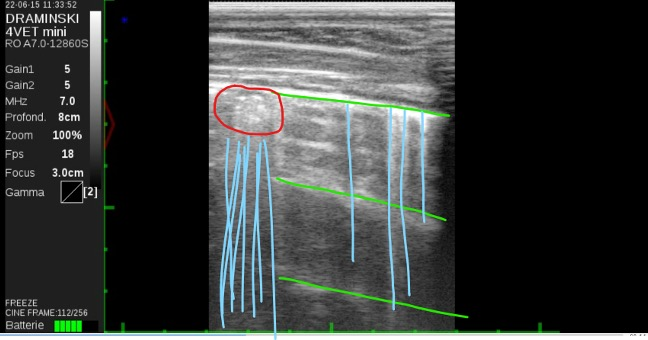
\includegraphics[width=\linewidth]{figures/chap2/annotated_ultrasound.jpg}
  \caption{Pulmonary ultrasound}
  \label{fig:ultrasound}
\end{figure}
\newpage

Achieving accurate and consistent results requires significant operator skill, training, and a systematic examination technique based on anatomical and ultrasonographic landmarks (fig \ref{fig:ultrasound}). Variations in operator skill levels can result in differing degrees of diagnostic accuracy and reliability, making standardized training and experience crucial for correct implementation


% Achieving accurate and consistent results requires significant operator skill, training, and a systematic examination technique based on anatomical and ultrasonographic landmarks. Variations in operator skill levels can result in differing degrees of diagnostic accuracy and reliability, making standardized training and experience crucial for correct implementation

This study therefore addresses two scientifically complementary research questions, directly inspired by contextual gaps and illustrated by our methodological contributions:

\paragraph{To what extent can deep learning reliably automate short-term diagnosis using limited, and context-specific observational data from sensors, such as lung ultrasounds ?} Unlike previous methods relying on manually extracted lesion characteristics \cite{timsit_association_2019}, our objective is to evaluate the extent to which deep learning architectures can autonomously derive high-level semantic representations from lung ultrasound videos.  We could then use this diagnosis expert to perform occasional diagnosis at different observation dates, this handles the need of a lot of data and could still provide first hand description of the health status (fig \ref{fig:chap2-question1}). We hypothesize that capturing the spatio-temporal patterns present in ultrasound videos through deep learning architectures can significantly enhance diagnostic robustness, particularly in field conditions where traditional manual lesion characterization is limited by subjectivity and variability. It might be lesion or it could another artefacts that the human eye wouldn't easily detect. This "sensor-to-diagnosis" automation could support veterinarians by offering immediate and objective assessments of animal health, providing valuable insight into the clinical state without extensive manual feature extraction or prolonged observational periods. Importantly, this approach could be practically deployed as a rapid and non-invasive technique to perform regular health monitoring, allowing veterinarians to obtain explicit, short-term descriptions of animal health status.

\begin{figure}
  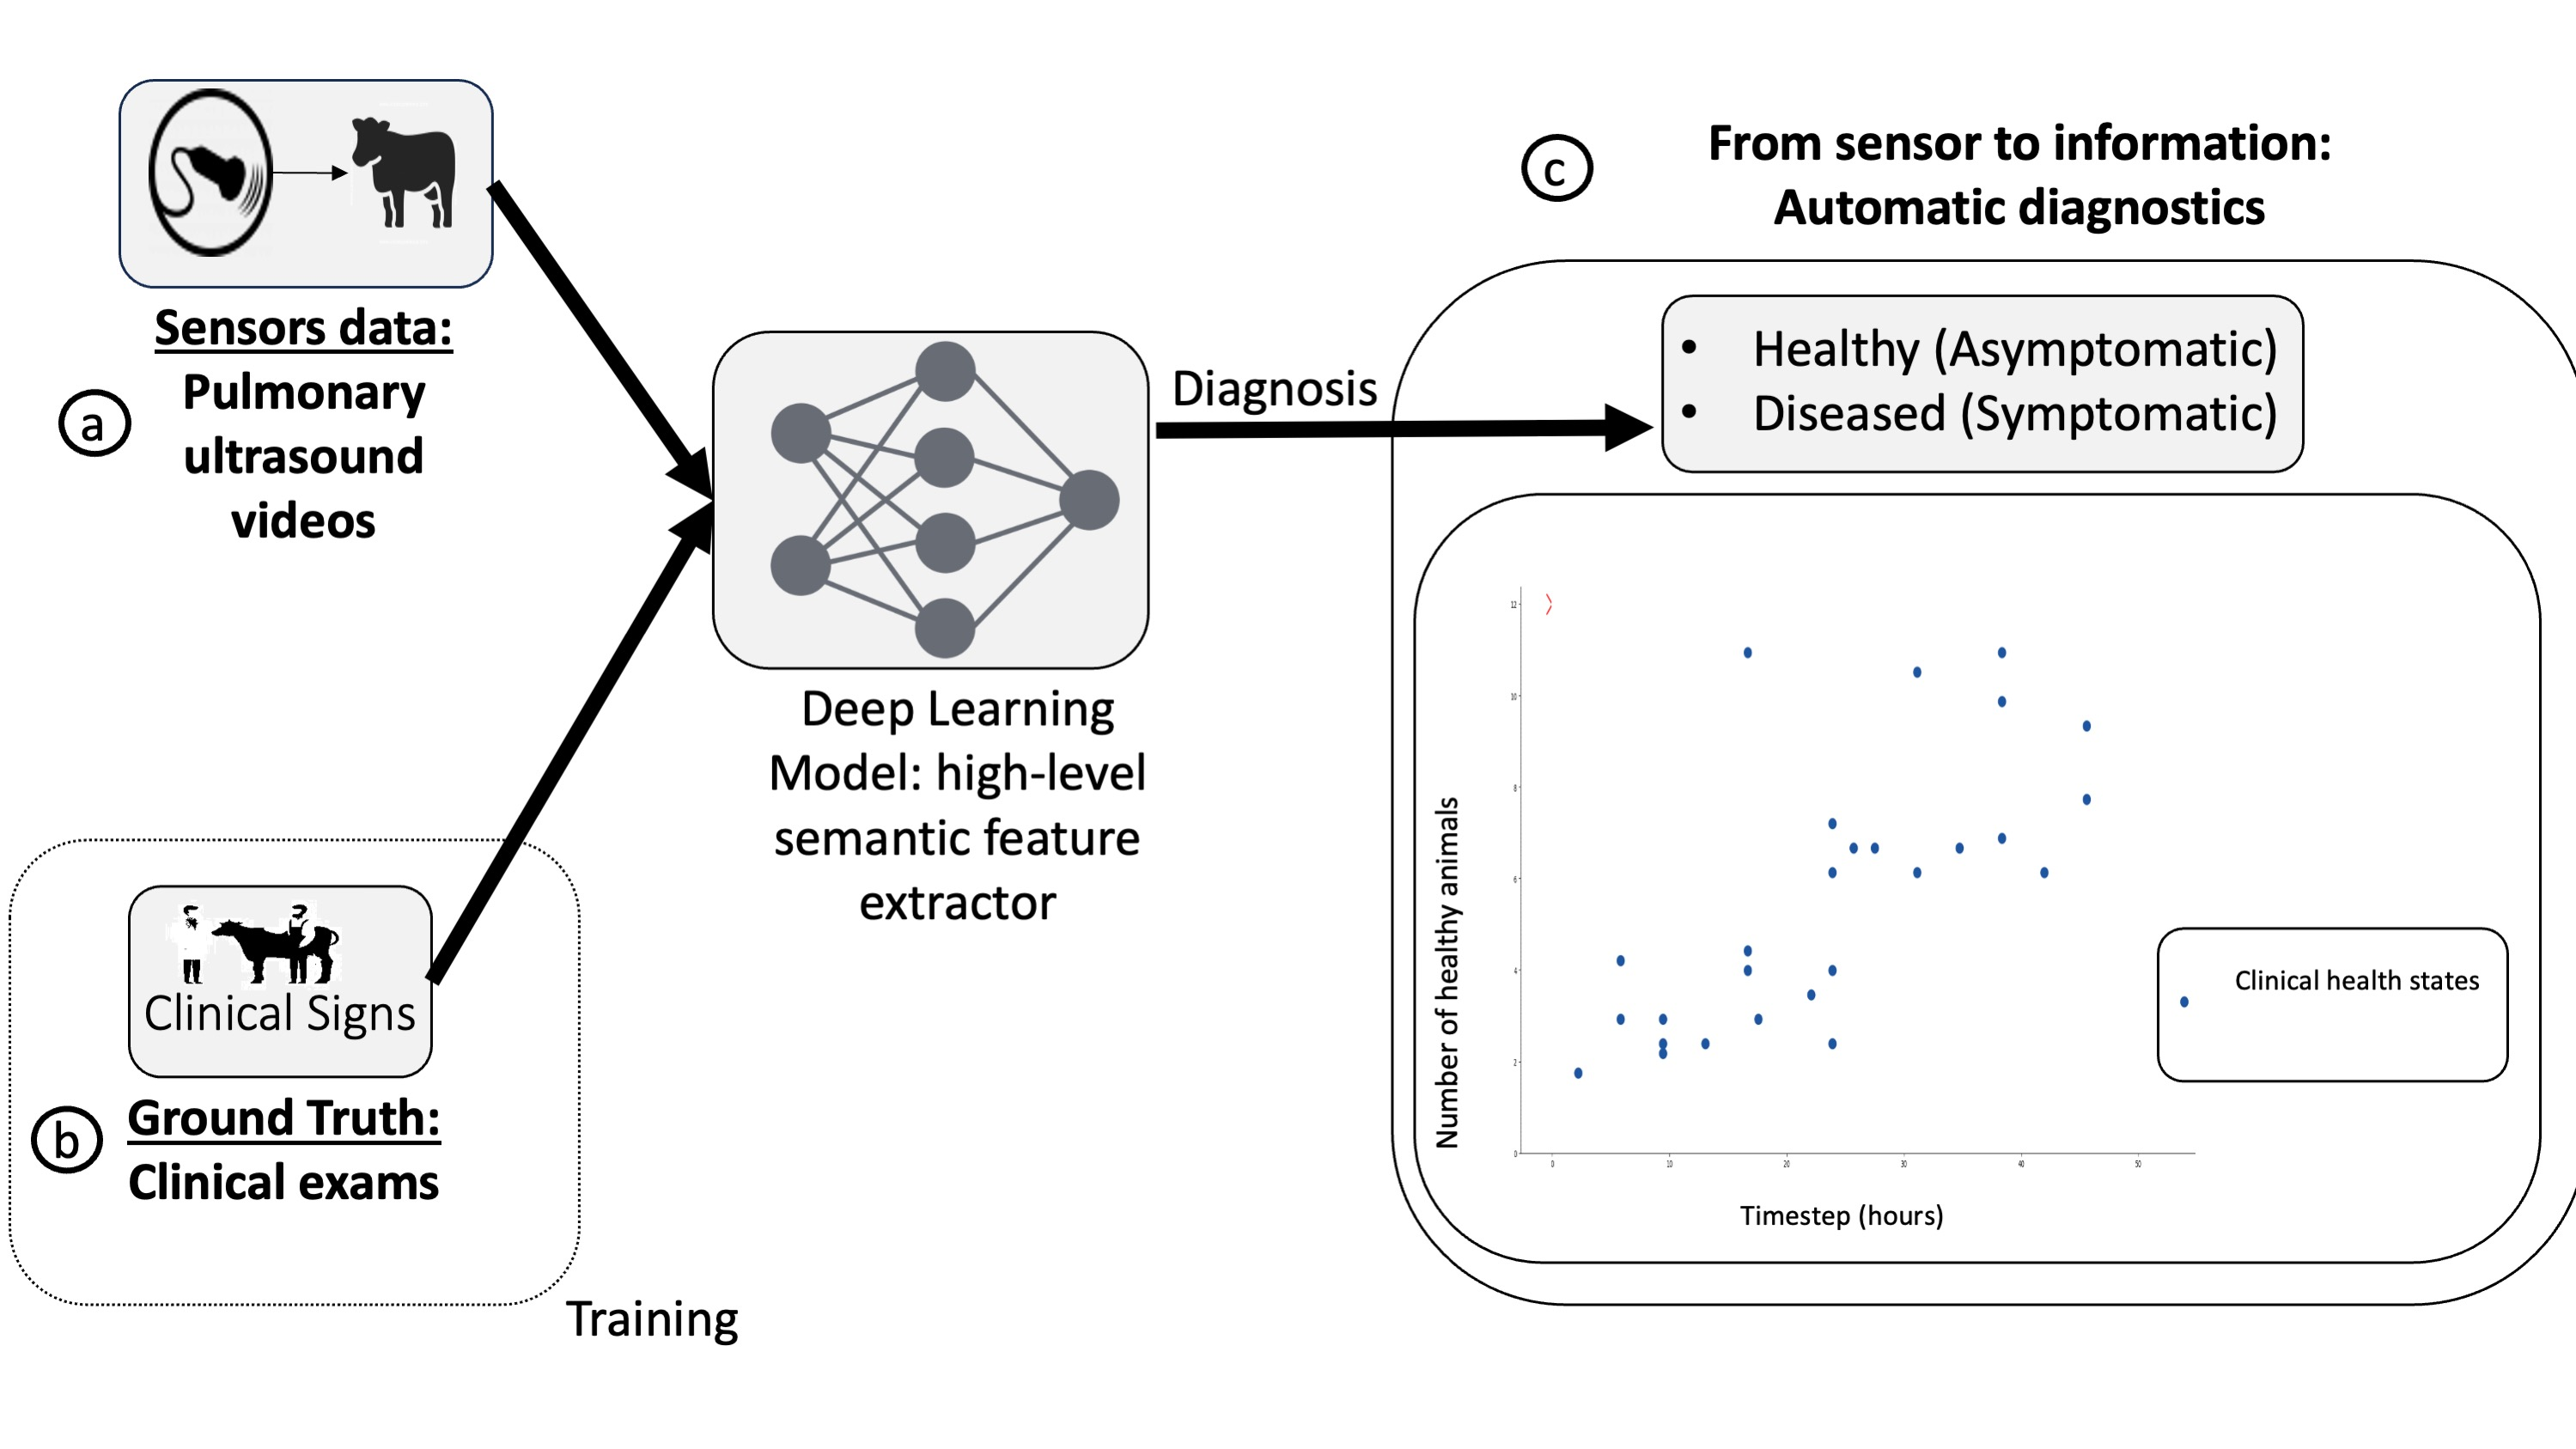
\includegraphics[width=\linewidth]{figures/chap2/chap1-question1.jpg}
  \caption{Can we use deep learning to automated the diagnosis at occasional date points using the limited available observations from sensors ?}
  \label{fig:chap2-question1}
\end{figure}
\newpage
    
\paragraph{Can mechanistic epidemiological models be parametrized using empirical veterinary observations to provide accurate explanatory long-term predictions for BRD ?} The previously established stochastic mechanistic model for BRD propagation \cite{picault_modelling_2022} was calibrated using theoretical assumptions rather than empirical veterinary observations, limiting its practical validation. In this work, we investigate whether empirical veterinary assessments considered ground truth, collected at limited temporal intervals and sparse frequency, can effectively parametrize a mechanistic epidemiological model to reliably predict BRD dynamics. Since daily health observations can be logistically challenging and costly in practice, we aim to assess whether accurate modelling can still be achieved by fitting the model to sparse empirical observations, allowing it to explicitly reconstruct disease dynamics and clinical states even on unobserved days (fig \ref{fig:chap2-question2}). Anything can happen in between the points, we could rely on the theoretical knowledge embedded in mechanistic models to explicit and give us evidence-based insights.


\begin{figure}
  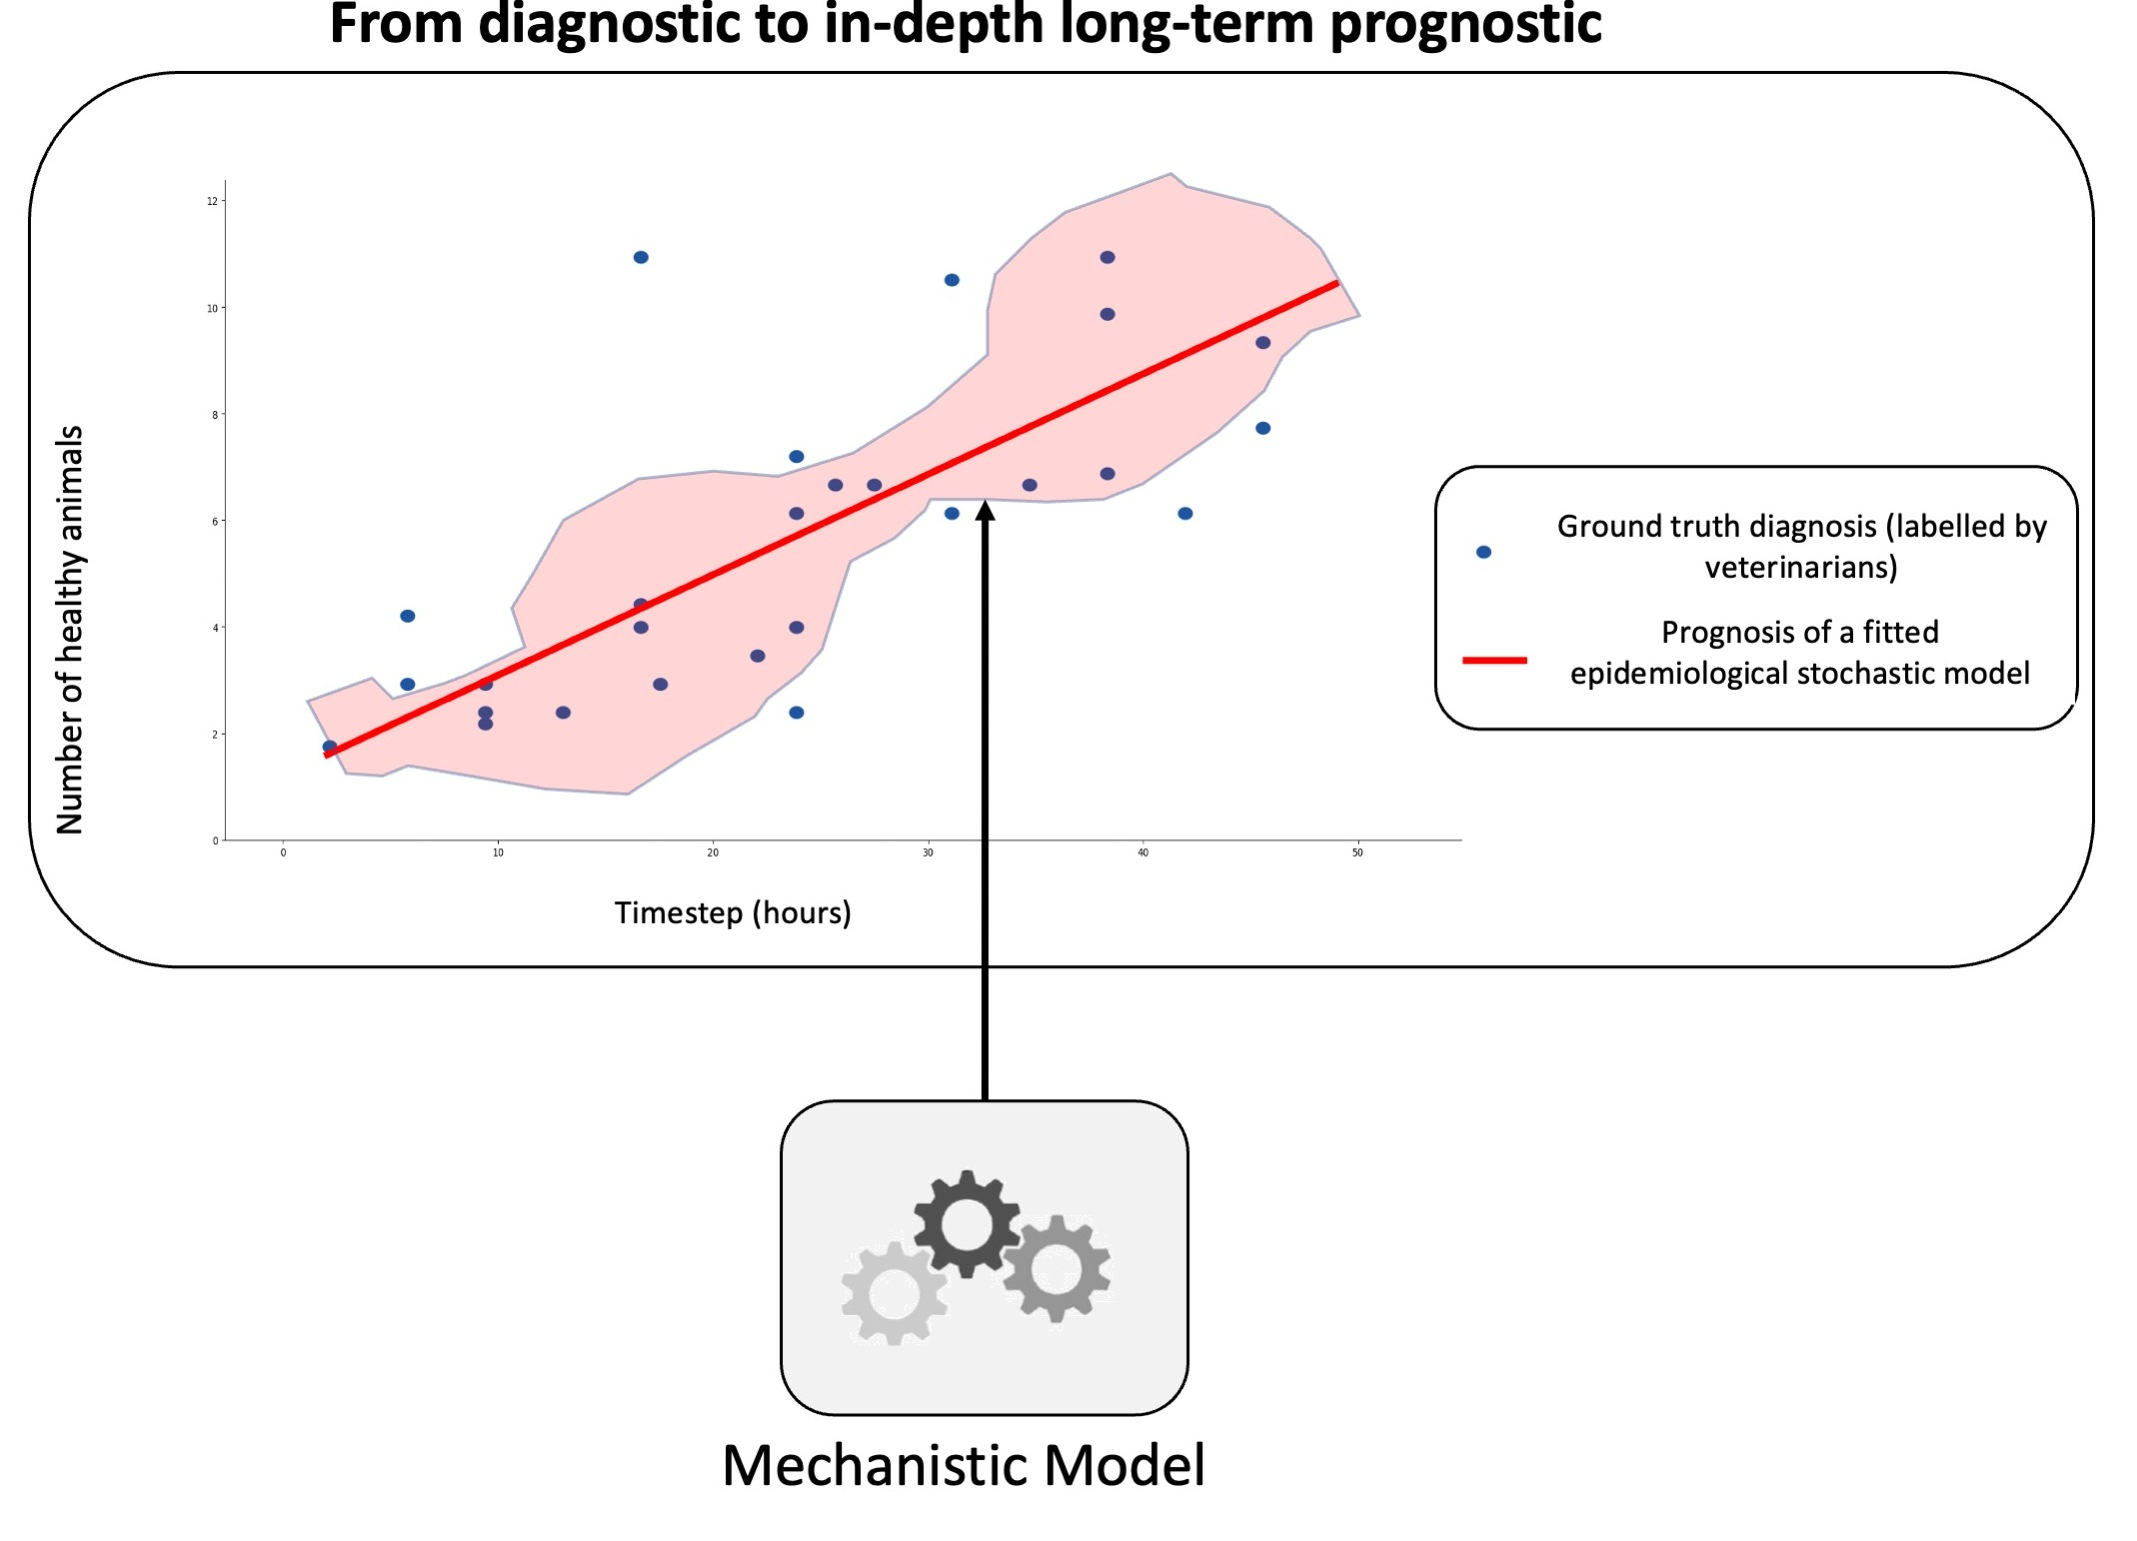
\includegraphics[width=\linewidth]{figures/chap2/chap1-question2.jpg}
  \caption{Can a mechanistic model for BRD be fitted to real-wolrd observations from veterinarians to predict at a larger temporal scale a explicit all the dynamics of BRD ?}
  \label{fig:chap2-question2}
\end{figure}
\newpage    


%-----------%-----------
%	SOUS-SECTION 
%-----------%-----------
\subsection{Main contributions and perspectives}
\label{chap:contributions}
This research provided three core contributions:

\begin{enumerate}
    \item Creation of an original dataset comprising pulmonary ultrasound videos with corresponding veterinary clinical annotations, providing a valuable resource for future BRD diagnostic and epidemiological research. Data collection occurred from January to June 2023, spanning a 30-day period post-arrival of calves on nine farms, each managing multiple batches of animals. Clinical annotations classified animals as symptomatic or asymptomatic according to veterinary-defined criteria (rectal temperature above 39.7°C and presence of at least one clinical symptoms such as cough or nasal discharge). Practical constraints, including animal immobilization, shaving the scan area, and veterinary availability, limited data quantity to approximately thirty annotated ultrasound videos. [\textcolor{red}{be more factual on the quantity of observation per class}]

    \item Veterinary clinical assessments enabled the parametrization of the BRD mechanistic epidemiological model \cite{picault_modelling_2022}. The sensitivity analysis conducted by Picault in 2022 revealed three parameters as the most influential in controlling BRD dynamics, antimicrobial usage, and mortality rates. These parameters are the \textbf{ pathogen transmission rate}, which describes how rapidly an infectious agent spreads between animals; the \textbf{mean duration in the infectious state}, representing how long an infected animal can transmit the disease; and the \textbf{mean duration in the pre-infectious state}, indicating how long an animal remains exposed before becoming actively infectious. Accurate estimation of these parameters is critical because they substantially influence infection spread, disease severity, and effectiveness of control strategies, including antimicrobial use. This parametrization (fig \ref{tab:parameter_comparison}) allowed predictions of BRD dynamics over a 30-day period, achieving forecasting accuracy with a root mean squared error (RMSE) below 5\% in certain farms. However, the general applicability of the average pathogen model across all scenarios warrants caution. We hypothesize that this simplification could limit its accuracy in predicting outbreaks driven primarily by viral infections. Indeed, Picault himself stated, "our assumption that the same 'average' pathogen could be used for all scenarios is indeed questionable. BRD is intrinsically a multi-pathogen disease, and the exact prevalence of each pathogen, their possible interactions, as well as the diversity of strains, can be expected to change the dynamics of infection and disease severity \cite{Kudirkiene2021, Becker2020}. In this study we assumed an average pathogen to keep the model as simple as possible. However, in further study, model parameters reflecting microbiological characteristics (e.g., the mean duration of infectiousness and the pathogen transmission rate) could be made pathogen-specific to allow for comparisons between various pathogens."

    \begin{table}[h]
        \centering
        \renewcommand{\arraystretch}{1.2}
        \begin{tabular}{l ccc ccc c}
            \toprule
            \multirow{2}{*}{\textbf{Parameter name}} & \multicolumn{3}{c}{\textbf{Farm 1}} & \multicolumn{3}{c}{\textbf{Farm 2}} & \multirow{2}{*}{\textbf{Nominal values}} \\
            
            \cmidrule(lr){2-4} \cmidrule(lr){5-7} 
            & Median & Q1 & Q3 & Median & Q1 & Q3 & Calibrated \\
            \midrule
            Pathogen Transmission rate & 0.009 & 0.006 & 0.012 & 0.019 & 0.014 & 0.023 & 0.008 \\
            Mean duration in infectious & 150 & 118 & 193 & 123 & 100 & 156 & 120 \\
            Mean duration in pre-infectious & 87 & 68 & 115 & 76 & 58 & 100 & 72 \\
            \bottomrule
        \end{tabular}
        \caption{Inferred values of parameters vs nominal value of parameters}
        \label{tab:parameter_comparison}
    \end{table}

    \begin{figure}[H]
      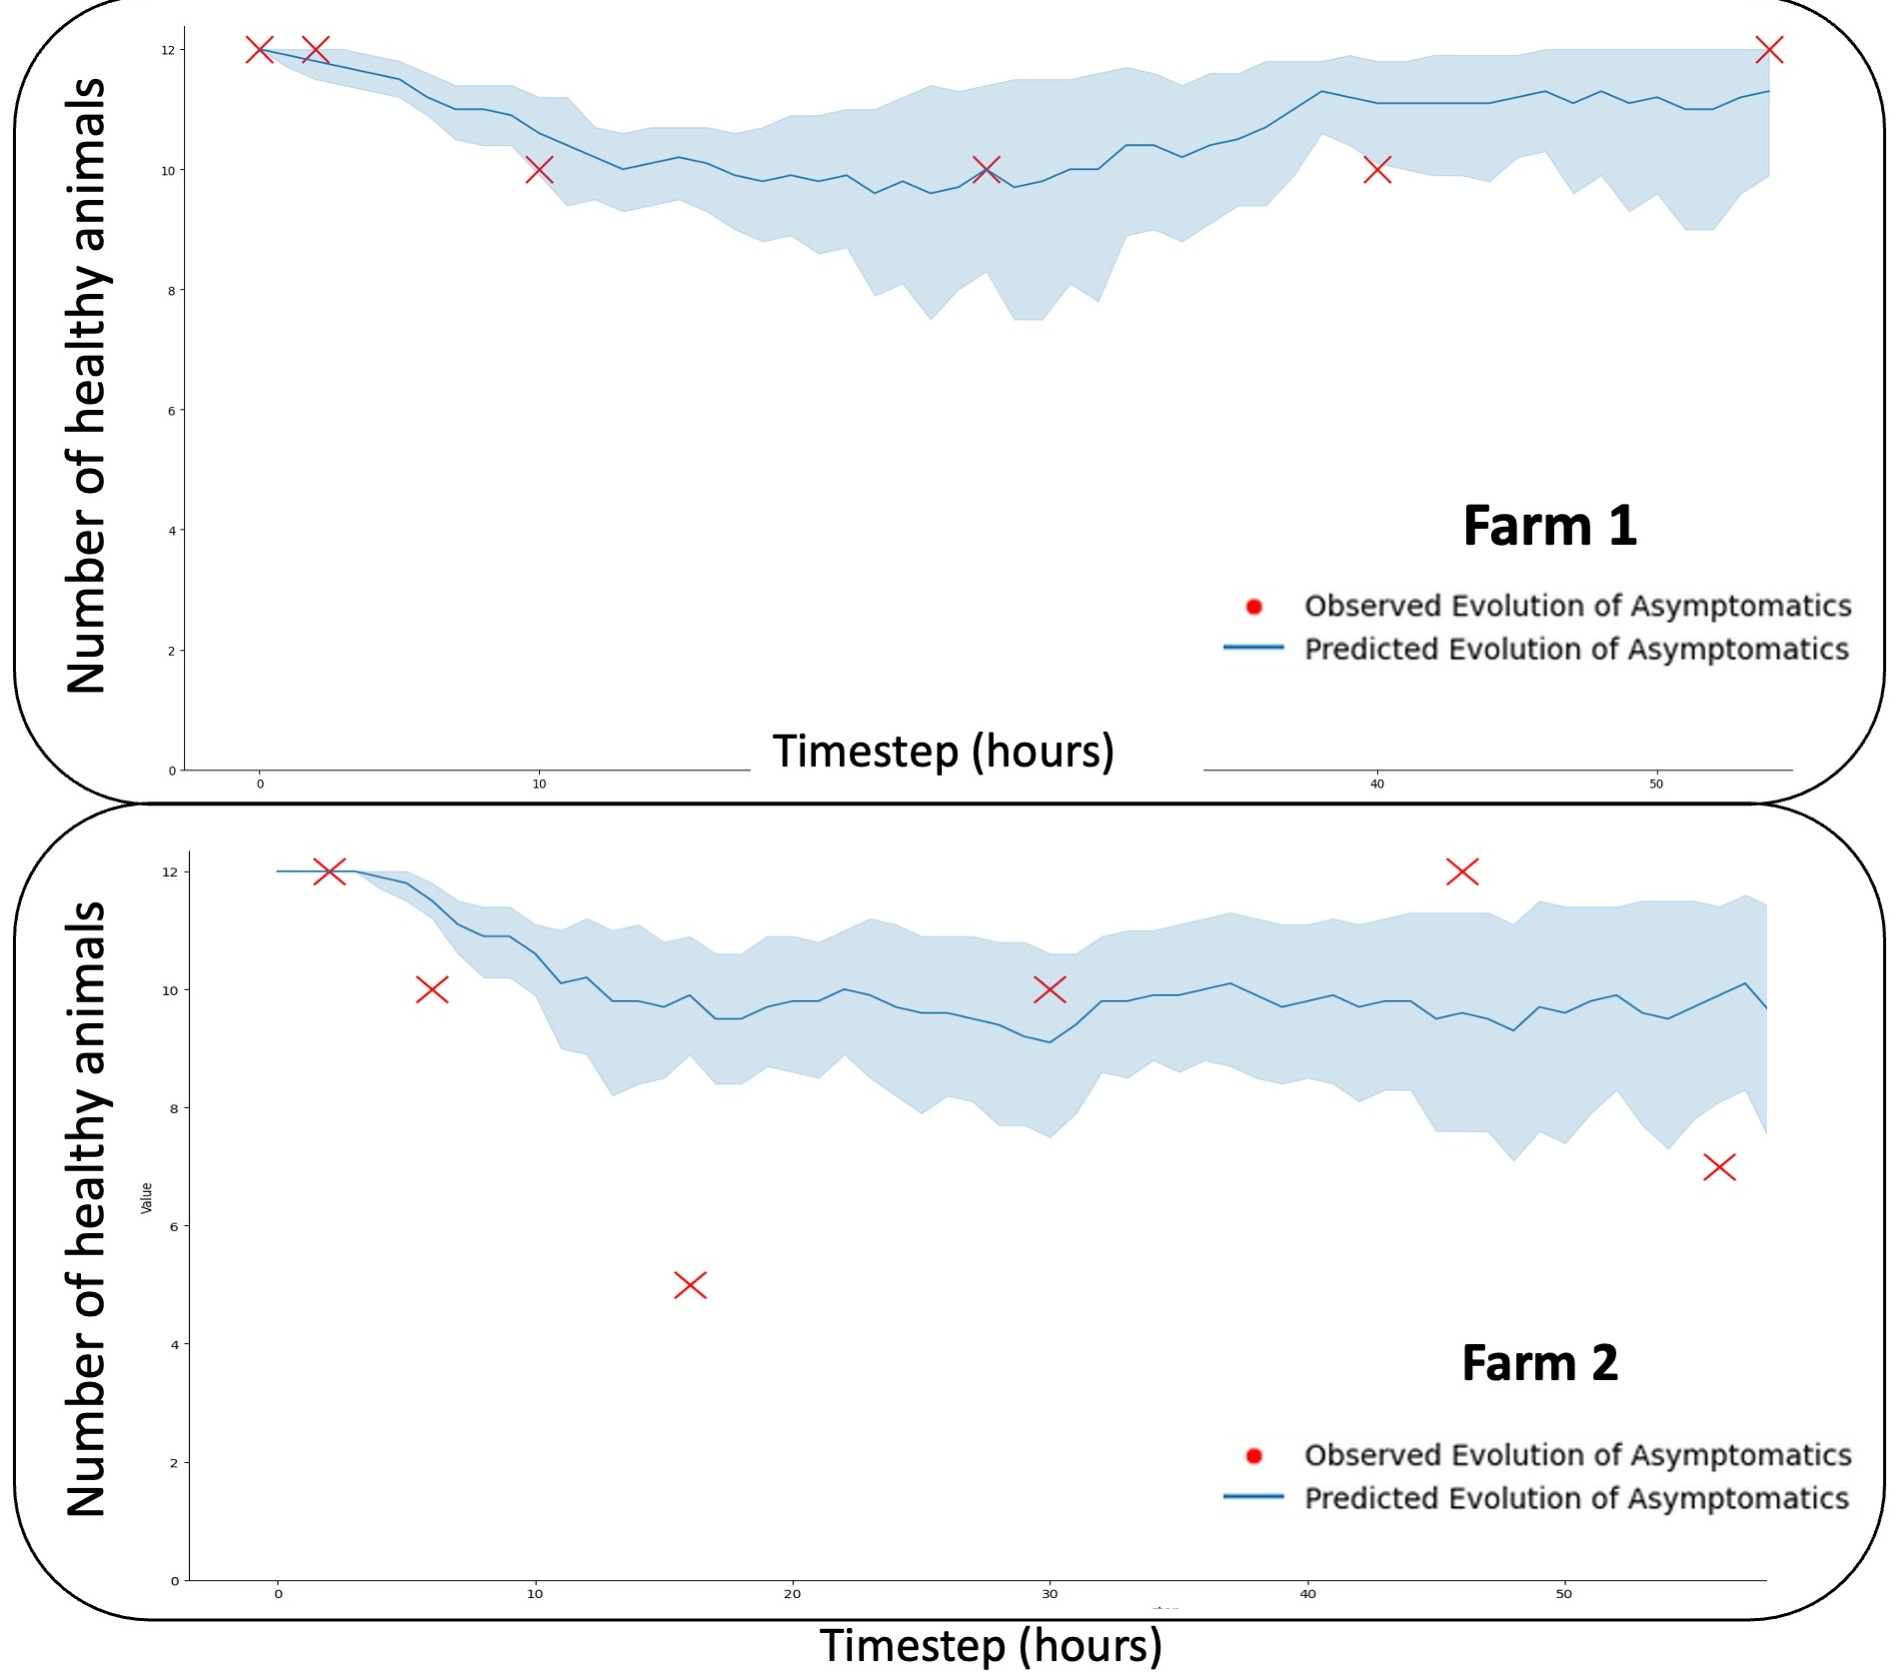
\includegraphics[width=\linewidth]{figures/chap2/prognosis-chap1.jpg}
      \caption{Asymptomatic forecast: ground truth vs predictions of an average pathogen mechanistic model}
      \label{fig:prognosis-chap1}
    \end{figure}

    \item A deep learning model based on a spatio-temporal CNN-RNN architecture was trained to classify animals’ clinical health status (symptomatic or asymptomatic) using pulmonary ultrasound videos. This model achieved an accuracy of approximately 72\% (table \ref{tab:feature_extractor_performance}). Specifically, the deep learning architecture combined convolutional neural networks (CNNs), serving as spatial feature extractors, and recurrent neural networks (RNN), which captured temporal information. Throughout the experiments, only the feature-extractor component—the CNN architecture—was varied, while the RNN architecture remained fixed across all tested models. The CNN's goal was to identify and extract relevant spatial features within individual ultrasound frames, such as lesions, pleura lines, or other anatomical details indicative of BRD. Conversely, the RNN aimed to leverage temporal sequences of these extracted features to model their evolution over the video duration. Different CNN architectures were evaluated, including EfficientNetB7, InceptionResnetV2, InceptionV3, VGG16, and an ensemble model combining InceptionV3 with InceptionResnetV2. Among these architectures, InceptionV3 achieved the highest performance, with a weighted F1-score of 70\%, precision of 72\%, recall of 69\%, and an overall accuracy of 69\%. In contrast, VGG16 demonstrated significantly lower performance, yielding an F1-score of only 14\%. The performance of the final selected deep learning model was assessed on two separate farms to verify its robustness and generalizability under contrasting practical conditions.
    
    \begin{table}[h]
        \centering
        \renewcommand{\arraystretch}{1.2} % Adjust row height for better readability
        \begin{tabularx}{\linewidth}{l *{4}{>{\centering\arraybackslash}X}}
            \toprule
            Feature Extractor & \small Weighted Precision & \small Weighted Recall & \small Weighted F1-score & \small Accuracy \\
            \midrule
            
            EfficientNetB7 & 0.67 & 0.62 & 0.63 & 0.62 \\
            InceptionResnetV2 & 0.71 & 0.50 & 0.49 & 0.50 \\
            InceptionV3 & \textbf{0.72} & \textbf{0.69} & \textbf{0.70} & \textbf{0.69} \\
            VGG16 & 0.09 & 0.31 & 0.14 & 0.31 \\
            InceptionV3 + InceptionResnetV2 & 0.71 & 0.62 & 0.63 & 0.62 \\
            
            \bottomrule
        \end{tabularx}
        \caption{Diagnosis performance of different deep learning architecture}
        \label{tab:feature_extractor_performance}
    \end{table}
    % \newpage 
        
\end{enumerate}

These results demonstrate the individual feasibility of both diagnostic automation using deep learning and epidemiological prognosis via mechanistic modelling. However, the two phases—diagnosis and prognosis—were not yet integrated into a complete predictive pipeline. Results highlighted the limitations of employing an average pathogen model universally, as BRD is intrinsically a multi-pathogen disease, and pathogen-specific variations significantly influence infection dynamics and disease severity. In the next chapter, methodologies for selecting the optimal prognosis expert model from multiple alternatives using outbreak observations will be discussed. 


% Pour ta thèse comme pour chaque chapitre, tu dois répondre à plusieurs questions impéra-tivement : 

% 1.	c'est quoi le problème ? (et dans quel contexte c'est un problème ?) à quelle question scientifique tu cherches à répondre ?

% 2.	en quoi c'est dur ?

% 3.	comment ça se positionne par rapport à l'existant : d'autres travaux / littérature (y compris par rapport à tes autres travaux pour le cas de chaque chapitre)

% 4.	quelles méthodes tu as employées, pourquoi, sous quelles hypothèses ?

% 5.	quels sont les résultats principaux ? en quoi ils apportent (ou pas) des éléments de réponse à la question (ou à d'autres questions) et quelles sont les questions qui se posent ensuite ?

% 6.	dans quelle mesure tes résultats sont-ils robustes ? quels sont les points faibles ou les limitations ? comment pourrait-on les corriger / contrebalancer (et est-ce nécessaire) ?

% 7.	enfin qu'est-ce qui resterait à explorer / faire ? quelles autres questions émergent à l'issue de ton travail ?

\subsection{[In French] Résumé grand public}

%-----------------------------------
%	SECTION 
%-----------------------------------

La maladie respiratoire bovine (BRD) est une pathologie fréquente et complexe qui représente un défi majeur en élevage, entraînant des pertes économiques importantes liées aux traitements, à la diminution des performances zootechniques et à une mortalité accrue. Afin de diagnostiquer cette maladie, les vétérinaires ont parfois recours à l’échographie pulmonaire, une méthode rapide, non invasive et réalisable directement à la ferme grâce à des appareils portables. Ces appareils, utilisés habituellement pour l'échographie reproductive chez les bovins, permettent d’examiner rapidement les poumons des animaux sans exposition à la radiation, contrairement à la radiographie ou au scanner. L’échographie pulmonaire peut identifier précisément et rapidement certaines lésions pulmonaires associées à la BRD, telles que la consolidation des lobes pulmonaires, les abcès ou encore les épanchements pleuraux. Ces lésions échographiques sont d’autant plus importantes qu’elles peuvent indiquer la gravité de la maladie, prédire les rechutes et renseigner sur les performances futures des animaux atteints.

Le projet SEPTIME, dans lequel s’inscrit ce travail de thèse, a permis la collecte de nombreuses données empiriques issues d’échographies pulmonaires enregistrées directement dans des élevages bovins durant les années 2023 et 2024. À partir de ces vidéos échographiques annotées par des vétérinaires experts, nous avons exploré deux approches complémentaires afin d’améliorer le diagnostic et le pronostic de la BRD :


\begin{enumerate} 
    \item L’utilisation de modèles d’intelligence artificielle (apprentissage profond) permettant d’automatiser rapidement la détection des cas cliniques de BRD à partir d’échographies pulmonaires. Ces modèles montrent un bon potentiel avec une précision atteignant environ 72\% dans la reconnaissance automatique de la maladie.

    \item Le paramétrage et l’évaluation d’un modèle mécaniste épidémiologique, qui simule la propagation à long terme de la maladie à partir d'observations réelles issues du terrain. Ce modèle mécaniste, une fois calibré, permet de prédire efficacement l’évolution de la maladie sur plusieurs semaines et pourrait ainsi aider les éleveurs à anticiper les épidémies et à adapter leurs stratégies de gestion sanitaire.

\end{enumerate}


Ces résultats démontrent la faisabilité individuelle de l'automatisation du diagnostic et du pronostic à l'aide de l'apprentissage profond et du pronostic épidémiologique via la modélisation mécaniste. Le chapitre suivant aborde les méthodologies de sélection du modèle expert de pronostic parmi de multiples alternatives en utilisant des observations cliniques.

\section{Proceedings published in Society for Veterinary Epidemiology and Preventive Medicine, 2024}


\includepdf[pages=-]{articles/SVEPM.pdf}  % Replace with your actual filename


% \chapter*{\Huge Big Title Here}
% \addcontentsline{toc}{chapter}{Big Title Here}  % Add to TOC if needed

\chapter{Structural synergism in bovine respiratory disease modelling} % chapter title

\section{Introduction}
\subsection{Contextual background}

%-----------
%	SOUS-SOUS-SECTION 
%------------

Mathematical modelling has emerged as a cornerstone for evidence-based decision-making in animal health, increasingly recognized as indispensable by policy makers and veterinary epidemiologists  \cite{Picault2024, Ezanno2022}. Modelling frameworks offer a structured approach to understanding disease dynamics, quantifying transmission risks, forecasting outbreaks, and evaluating intervention strategies. In veterinary epidemiology, and particularly in the management of complex multi-pathogen diseases like Bovine Respiratory Disease (BRD), mathematical models serve as powerful tools that integrate knowledge across multiple disciplines, including epidemiology, veterinary science, agricultural management, and economics.

BRD is inherently complex due to its multifactorial nature, characterized by interactions between various pathogens, host susceptibility, environmental stressors, and management practices. Numerous mechanistic epidemiological models have been proposed to capture this complexity \cite{picault_modelling_2022, sorindupont_modeling_2023}. However, the mechanisms governing pathogen interactions, co-infections, and the clinical manifestations of BRD remain incompletely understood. Consequently, existing models often differ significantly in their structure, underlying assumptions, and levels of biological detail. These structural differences create uncertainties in predictions, complicating the practical task of identifying a model that accurately reflects real-world outbreak dynamics.

Recent developments emphasize the advantages of using pathogen-specific mechanistic models instead of generalized "average pathogen" approaches. Pathogens such as Orthopneumovirus bovis (BRSV), Mannheimia haemolytica (Mh), and Mycoplasmopsis bovis (Mb) exhibit distinct epidemiological characteristics, clinical progressions, and treatment responses, each requiring targeted intervention strategies. Recognizing this diversity, pathogen-specific models have been advocated for their enhanced realism and predictive accuracy in simulating BRD outbreaks. Beyond parameterization challenges, the comparative assessment of multiple valid mechanistic models necessitates addressing critical methodological dimensions. Model distinguishability, assesses whether competing models produce sufficiently distinct predictions, thereby enabling pathogen-model identification from clinical observations. Secondly, and most practically relevant, is the concept of decision impact assessment, evaluating whether the selection of a given model actually translates into measurable, economically viable, and actionable improvements on the farm. These two interconnected methodological challenges underscore the need not only for rigorously validated mechanistic models but also for frameworks capable of linking theoretical model selection directly with improved decision-making outcomes.




\subsection{Originality and objective of this work}
%-----------%-----------
%	SOUS-SECTION 
%-----------%-----------

this chapter focuses on two scientifically complementary research questions, driven by critical contextual and methodological challenges highlighted above:

\paragraph{To what extent can we reliably differentiate between multiple pathogen-specific mechanistic models of BRD, solely based on symptomatic observations ?} In this chapter, we introduce a numerical approach aimed at distinguishing among competing BRD mechanistic epidemiological models \cite{sorindupont_modeling_2023} based exclusively on observed symptomatic trajectories. Specifically, we show a general theoretical framework for pathogen-model identification, a critical issue across epidemiological contexts where accurate differentiation between pathogens is challenged by symptom overlap. The relevance of this work extends beyond Bovine Respiratory Disease (BRD), offering a broadly applicable solution for any epidemiological scenario involving multiple plausible mechanistic hypotheses or co-existing pathogens that necessitate distinct pathogen-specific management strategies. Orthopneumovirus bovis (BRSV) model captures rapid, airborne viral transmission dynamics, characterized by acute and intense infection episodes. It explicitly incorporates compartments for partial immunity, primary infection, potential reinfection (with reduced infectiousness), and rapid progression from mild to severe clinical signs, making the outbreaks swift but relatively short-lived. Mannheimia haemolytica (Mh) is modelled as an opportunistic infection primarily triggered by host immunosuppression or environmental stressors. Unlike the BRSV model, the Mh model does not account for reinfection states but includes a clear transition from asymptomatic carriage to active infection states, which can escalate into severe clinical manifestations. The infection dynamics are less explosive compared to BRSV, emphasizing progression triggered by stress-induced susceptibility. The mycoplasmosis bovis (Mb) model structurally mirrors the Mh model regarding compartments (asymptomatic carriers transitioning to symptomatic stages). However, it notably differs by emphasizing chronicity and persistence. This pathogen exhibits slower transmission, prolonged infection durations, and intermittent clinical symptom manifestation, making early detection and timely treatment more challenging and resulting in prolonged circulation within cattle populations. The probability that a treated animal recovers (for 1 dose) is set to 71\% for  Mh and 60\% for Mb. The models where calibrated using from the litterature: probabilities of recovery with antibiotic treatment (single dose) are set at 71\% for Mh and 60\% for Mb. the probability of detecting symptomatic animals (with mild clinical signs) is ... and the probability of detecting a animal displaying severe clinical signs is ...


\paragraph{Does the distinction and identification of the most likely pathogen-specific mechanistic model significantly improve practical decision-making outcomes ?} In typical cattle farming practices (conventional treatment decisions), antibiotic treatments for Bovine Respiratory Disease (BRD) are usually administered empirically based solely on observable clinical signs, without reliable pathogen identification. Under these conditions, farmers treat all symptomatic animals with antibiotics, regardless of whether the underlying infectious agent is bacterial or viral. Since antibiotics are effective only against bacteria and not viruses, this approach frequently leads to inappropriate use of antibiotics, which has two main drawbacks: if the infectious agent is viral, antibiotic treatments are unnecessary, ineffective, and economically wasteful. Such misuse increases antimicrobial resistance risks without any animal health benefit. If the infectious agent is bacterial, antibiotics are warranted and beneficial; failure to correctly administer them could lead to severe economic losses and compromised animal welfare.

To address this issue, we explicitly incorporate an economic dimension into our analysis by integrating pathogen-specific model predictions into a bio-economic framework. This enables us to quantify practical benefits, such as reductions in antibiotic usage, improved animal health outcomes, and enhanced profitability directly resulting from pathogen-informed decisions. By explicitly evaluating these consequences, our work connects theoretical epidemiological modelling with tangible, farm-level decision-making, reinforcing the practical relevance of modelling for effective livestock management.


% cite to articles discussing about cholera model distinguishability. [explain the difference between model selection and model distinguishability.]


\subsection{Main contributions and perspectives}

\subsubsection*{prognostic expert identification via model distinguishability}

Our primary methodological contribution involves numerically distinguishing three mechanistic BRD models tailored for Orthopneumovirus bovis (BRSV), Mannheimia haemolytica (Mh), and Mycoplasmopsis bovis (Mb) \cite{sorindupont_modeling_2023}. First, We constructed synthetic outbreak scenarios representative of French beef cattle farms. Three discrete-time, stochastic agent-based, pathogen-specific model  were utilized to generate outbreak trajectories over 277 days, capturing symptomatic dynamics every 12 hours for a batch of 12 calves. Variations across scenarios reflected realistic risk compositions, yielding a dataset comprising 13,650 individual simulations. Secondly, Three pathogen-specific stochastic, compartmental models \cite{sorindupont_modeling_2023} were compared, each encapsulating different transmission dynamics. Given the stochastic complexity of models and intractable likelihood functions, we employed Approximate Bayesian Computation (ABC) combined with multinomial logistic regression to identify the most likely pathogen-specific model. The ABC approach quantitatively assessed model distinguishability using summary statistics (detected symptomatic trajectories), thus allowing informed selection of the pathogen responsible for observed outbreaks.Given the stochastic complexity of models and intractable likelihood functions, we employed Approximate Bayesian Computation (ABC) combined with multinomial logistic regression to identify the most likely pathogen-specific model. The ABC approach quantitatively assessed model distinguishability using summary statistics (detected symptomatic trajectories), thus allowing informed selection of the pathogen responsible for observed outbreaks. Using synthetic symptomatic data generated under realistic farm conditions, we successfully identify the most likely pathogen-specific model with an average accuracy of approximately 93\% (fig \ref{fig:chap3-confusion-matrix}). Key performance metrics (true positive rates: BRSV=96\%, Mh=90\%, Mb=87\%) clearly indicate the feasibility and reliability of pathogen identification based on early symptomatic trajectories.

\begin{figure}[H]
  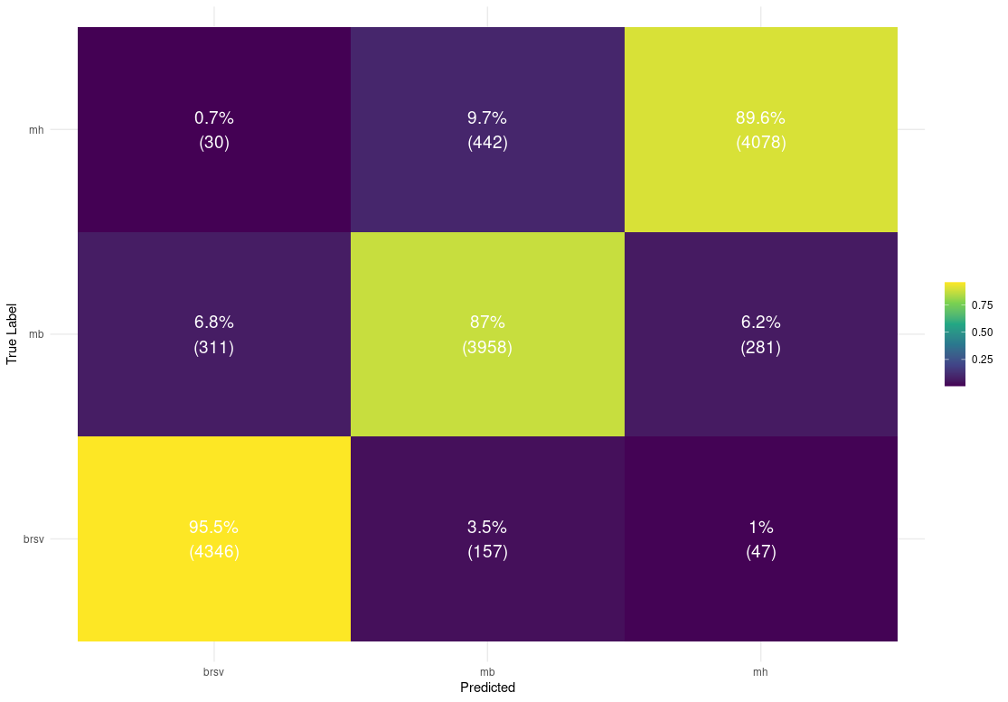
\includegraphics[width=\linewidth]{figures/chap3/chap3-confusionmatrix.png}
  \caption{Confusion matrix. Classification performance for BRSV, Mh and Mb. The diagonal represents correctly classified instances, while off-diagonal values indicate misclassification between classes.}
  \label{fig:chap3-confusion-matrix}
\end{figure}


\subsubsection*{Decision-intelligence: measuring and improving the impact on decision-making}

The second major contribution involves integrating pathogen-specific epidemiological models into a detailed economic evaluation framework. This integration enables us to quantitatively assess the economic impact of adopting pathogen-informed treatment decisions versus conventional empirical treatment strategies. Our economic model accounts explicitly for weight gain, carcass quality, feed, antibiotic treatment costs, and veterinarian interventions, calculating expected net profits and antibiotic usage for simulated cattle batches. We showed that pathogen-informed decisions substantially reduce antimicrobial use by approximately 44\% (fig \ref{fig:chap3-expectation}) in these conditions, directly addressing critical issues like antimicrobial resistance and public health safety. Simultaneously, these pathogen-informed strategies lead to a modest yet consistent increase (around 1\%) in net profitability, highlighting that economic viability can be maintained or improved even when reducing antibiotic treatments.

By leveraging the high accuracy (~93\%) of pathogen-model distinguishability, we maximize the likelihood that the correct treatment decision, either antibiotic administration for bacterial infections or withholding antibiotics for viral infections—is consistently taken.This accuracy directly improves decision-making outcomes by: Increasing the frequency of correct recommendations, thus ensuring targeted treatments that align with actual disease aetiology. And reducing incorrect or harmful decisions (false positives and false negatives), significantly decreasing inappropriate antibiotic use and associated economic and public health costs.

\begin{figure}[H]
  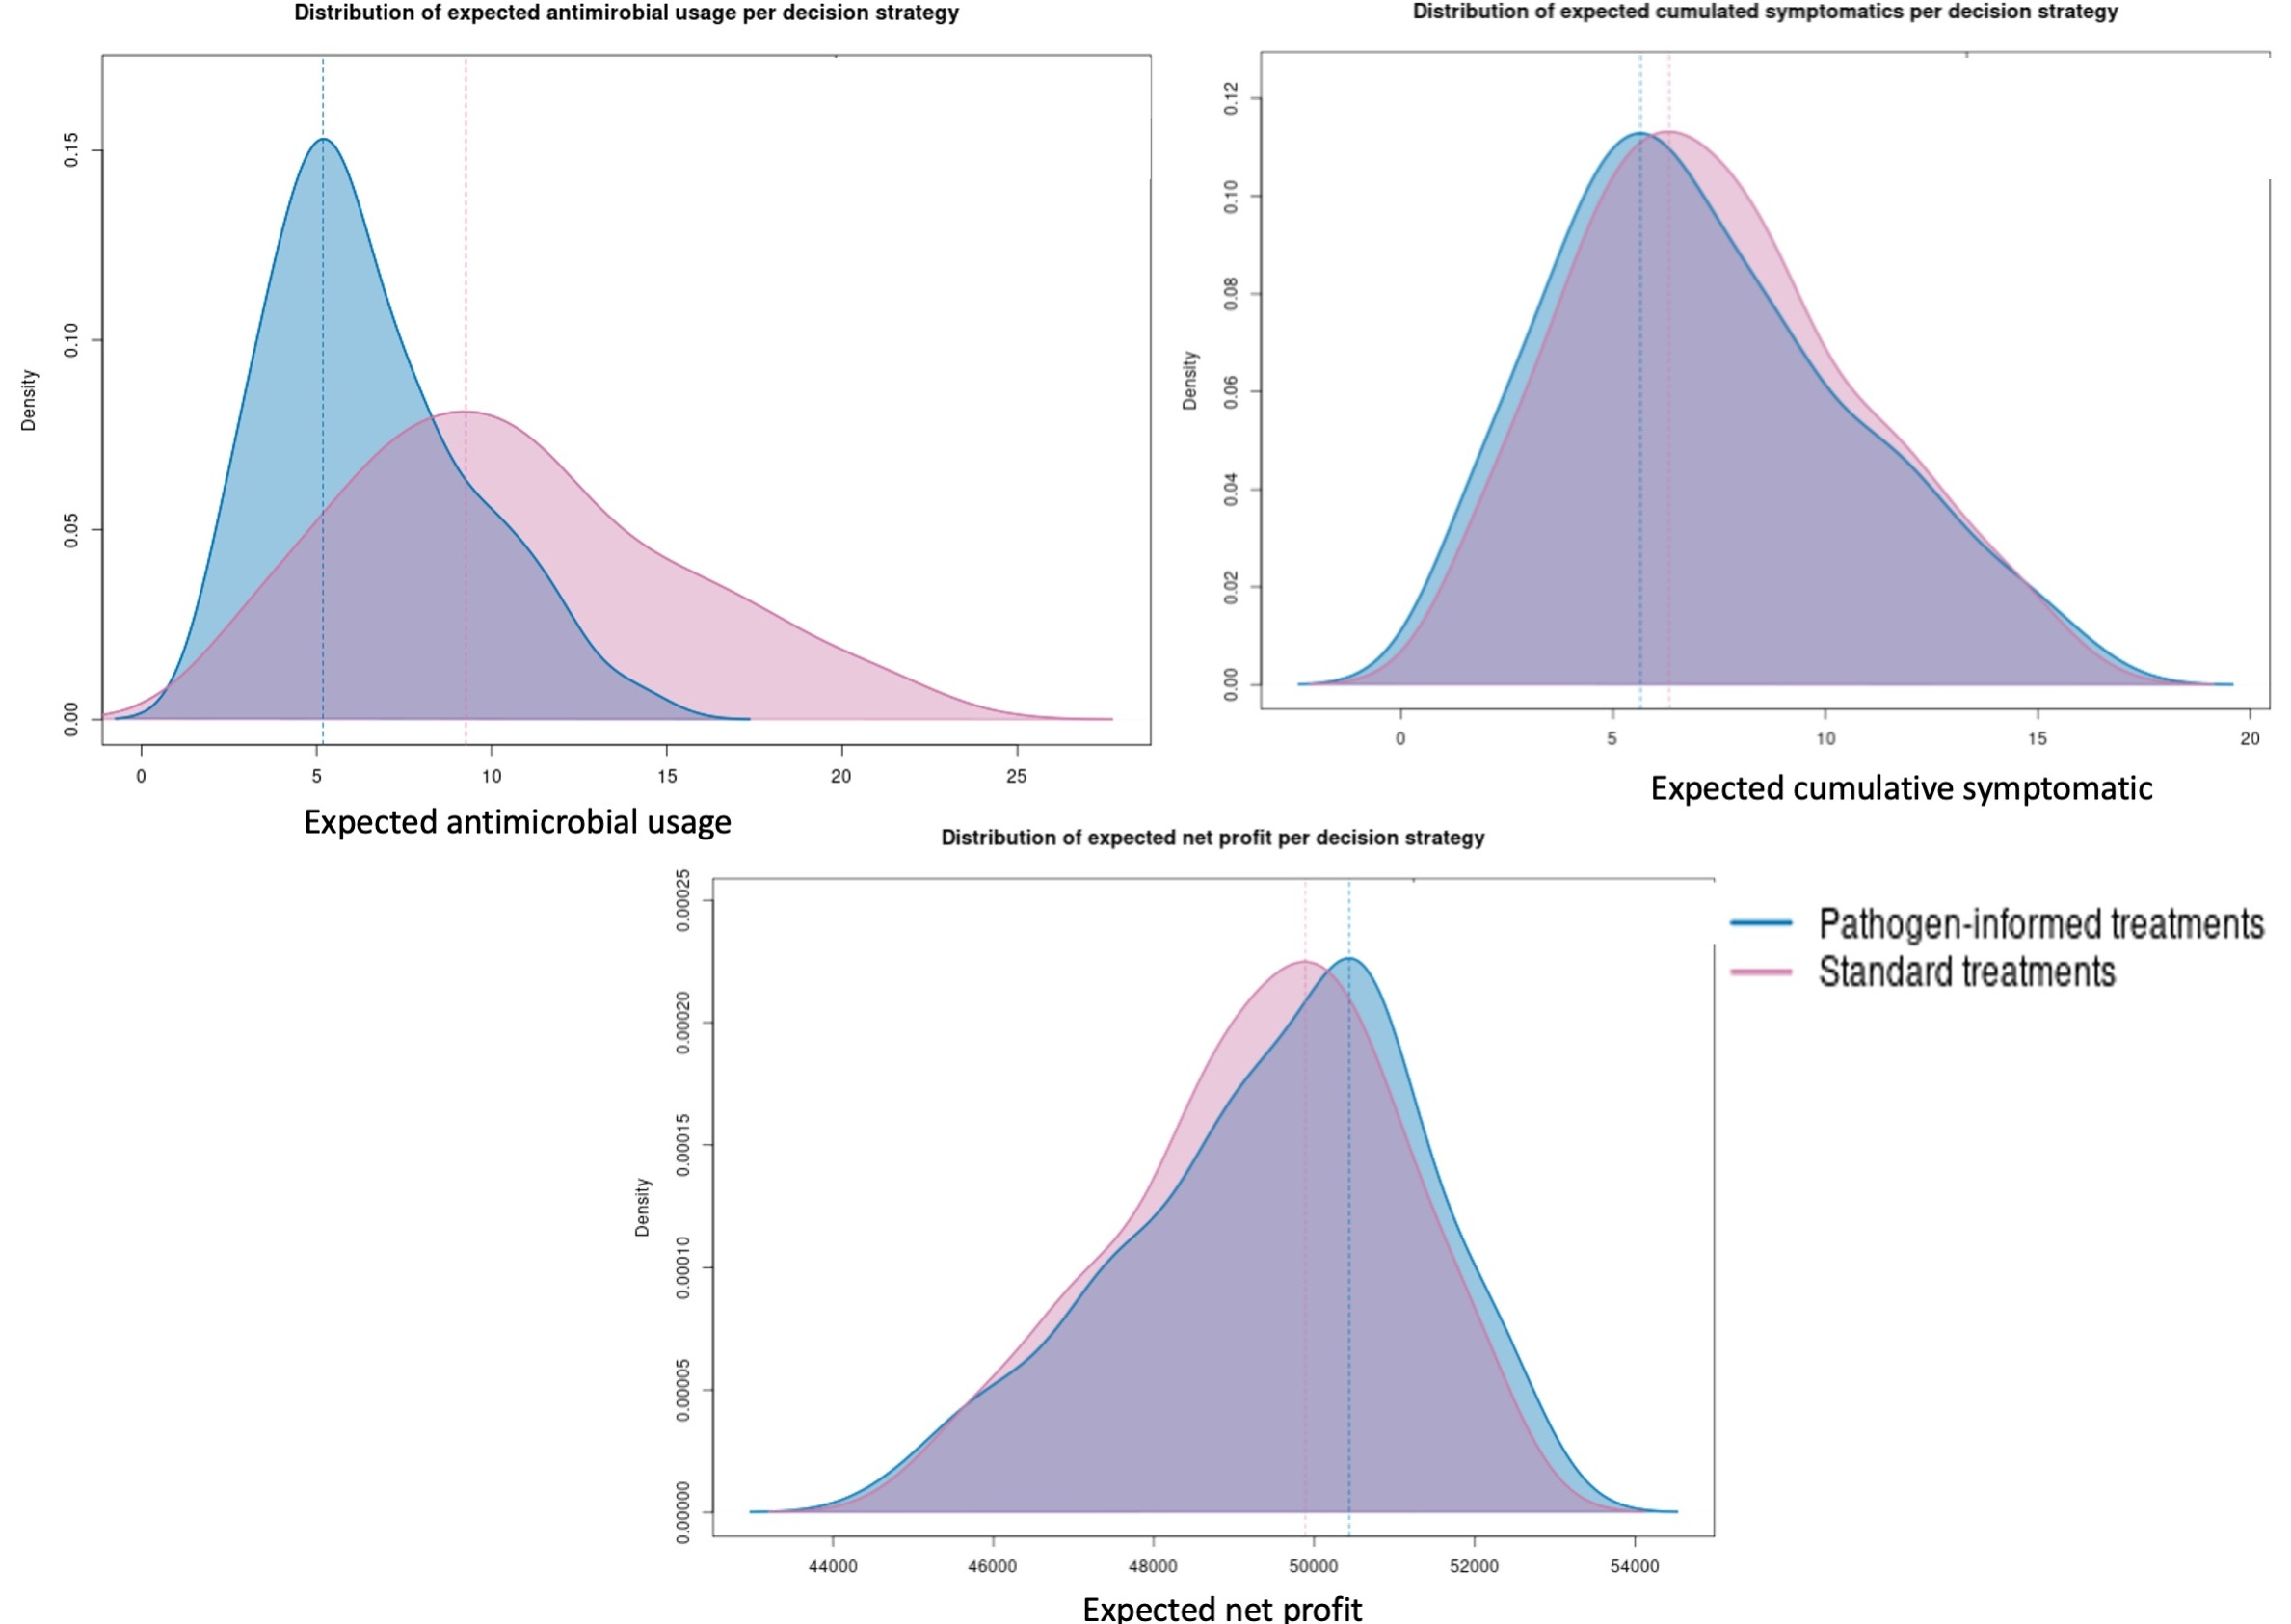
\includegraphics[width=\linewidth]{figures/chap3/expectations.jpg}
  \caption{Pathogen informed treatment decisions versus conventional treatment decisions.}
  \label{fig:chap3-expectation}
\end{figure}

\subsubsection*{Perspectives}

This work bridges theoretical epidemiological modelling with practical decision-making, emphasizing the importance of model distinguishability not only theoretically but as a practical tool for veterinary epidemiology and livestock management. Our approach is broadly applicable to scenarios where pathogen differentiation based solely on observations remains challenging yet essential. In the next chapter, we further explore integrating a real-world observation (sensor-based) for immediate diagnostic insights (deep learning-driven) with longer-term, prognosis-oriented mechanistic epidemiological models, combining these two forms of expertise to generate actionable disease management recommendations.

\subsection{[In French] Résumé grand public}
La gestion efficace des maladies respiratoires bovines (BRD) constitue un enjeu crucial pour la santé animale et pour l’économie des élevages bovins. Ces maladies sont complexes car elles impliquent souvent plusieurs pathogènes différents, notamment des virus comme Orthopneumovirus bovis (BRSV), et des bactéries telles que Mannheimia haemolytica (Mh) ou Mycoplasmopsis bovis (Mb). Chaque pathogène possède ses propres particularités en matière de transmission, de symptômes et de réponse au traitement, rendant leur identification précise essentielle pour une gestion optimale.

Dans ce chapitre, nous avons proposé une approche basée sur la modélisation mécaniste afin d’identifier quel pathogène est à l’origine d’une épidémie, simplement à partir des symptômes observés chez les animaux. Notre méthode utilise des modèles mécanistes spécifiques à chaque pathogène, pour déterminer avec fiabilité l’agent responsable d’une épidémie sur une exploitation. Grâce à des simulations numériques réalistes, nous avons montré que cette identification est possible avec une précision élevée (environ 93\% en moyenne).

Cette identification précise présente des avantages pratiques majeurs pour les éleveurs. Aujourd'hui, faute d’identification fiable, les traitements antibiotiques sont souvent administrés à tous les animaux symptomatiques sans distinction, même si certains souffrent d’infections virales pour lesquelles les antibiotiques sont inefficaces. Cette pratique entraîne une utilisation excessive et inutile des antibiotiques, augmentant le risque de résistance bactérienne, tout en générant des coûts économiques inutiles. Notre étude démontre que l’intégration de ces modèles spécifiques dans une démarche décisionnelle permet une réduction d'environ 44\% de la consommation d’antibiotiques tout en maintenant, voire en augmentant légèrement (~1\%), la rentabilité des exploitations.

Ainsi, ce travail met en évidence l’intérêt concret des modèles mécanistes pour améliorer les décisions pratiques en élevage, réduisant à la fois les coûts économiques et les risques sanitaires liés à une mauvaise utilisation des traitements. Cette approche pourrait s’appliquer à d’autres contextes épidémiologiques où identifier précisément le pathogène à partir de simples observations cliniques reste un défi majeur.


%-----------------------------------
%	SECTION 
%-----------------------------------
\section{Peer-reviewed preprint in bioarxiv, 2025}


    % \input{chapters/chap1-article} # pas besoin de mettre un file appart sauf si j'ai des choses spécifiques à rajouter pour cette partie
    \includepdf[pages=-]{articles/article3.pdf}  % Replace with your actual filename
    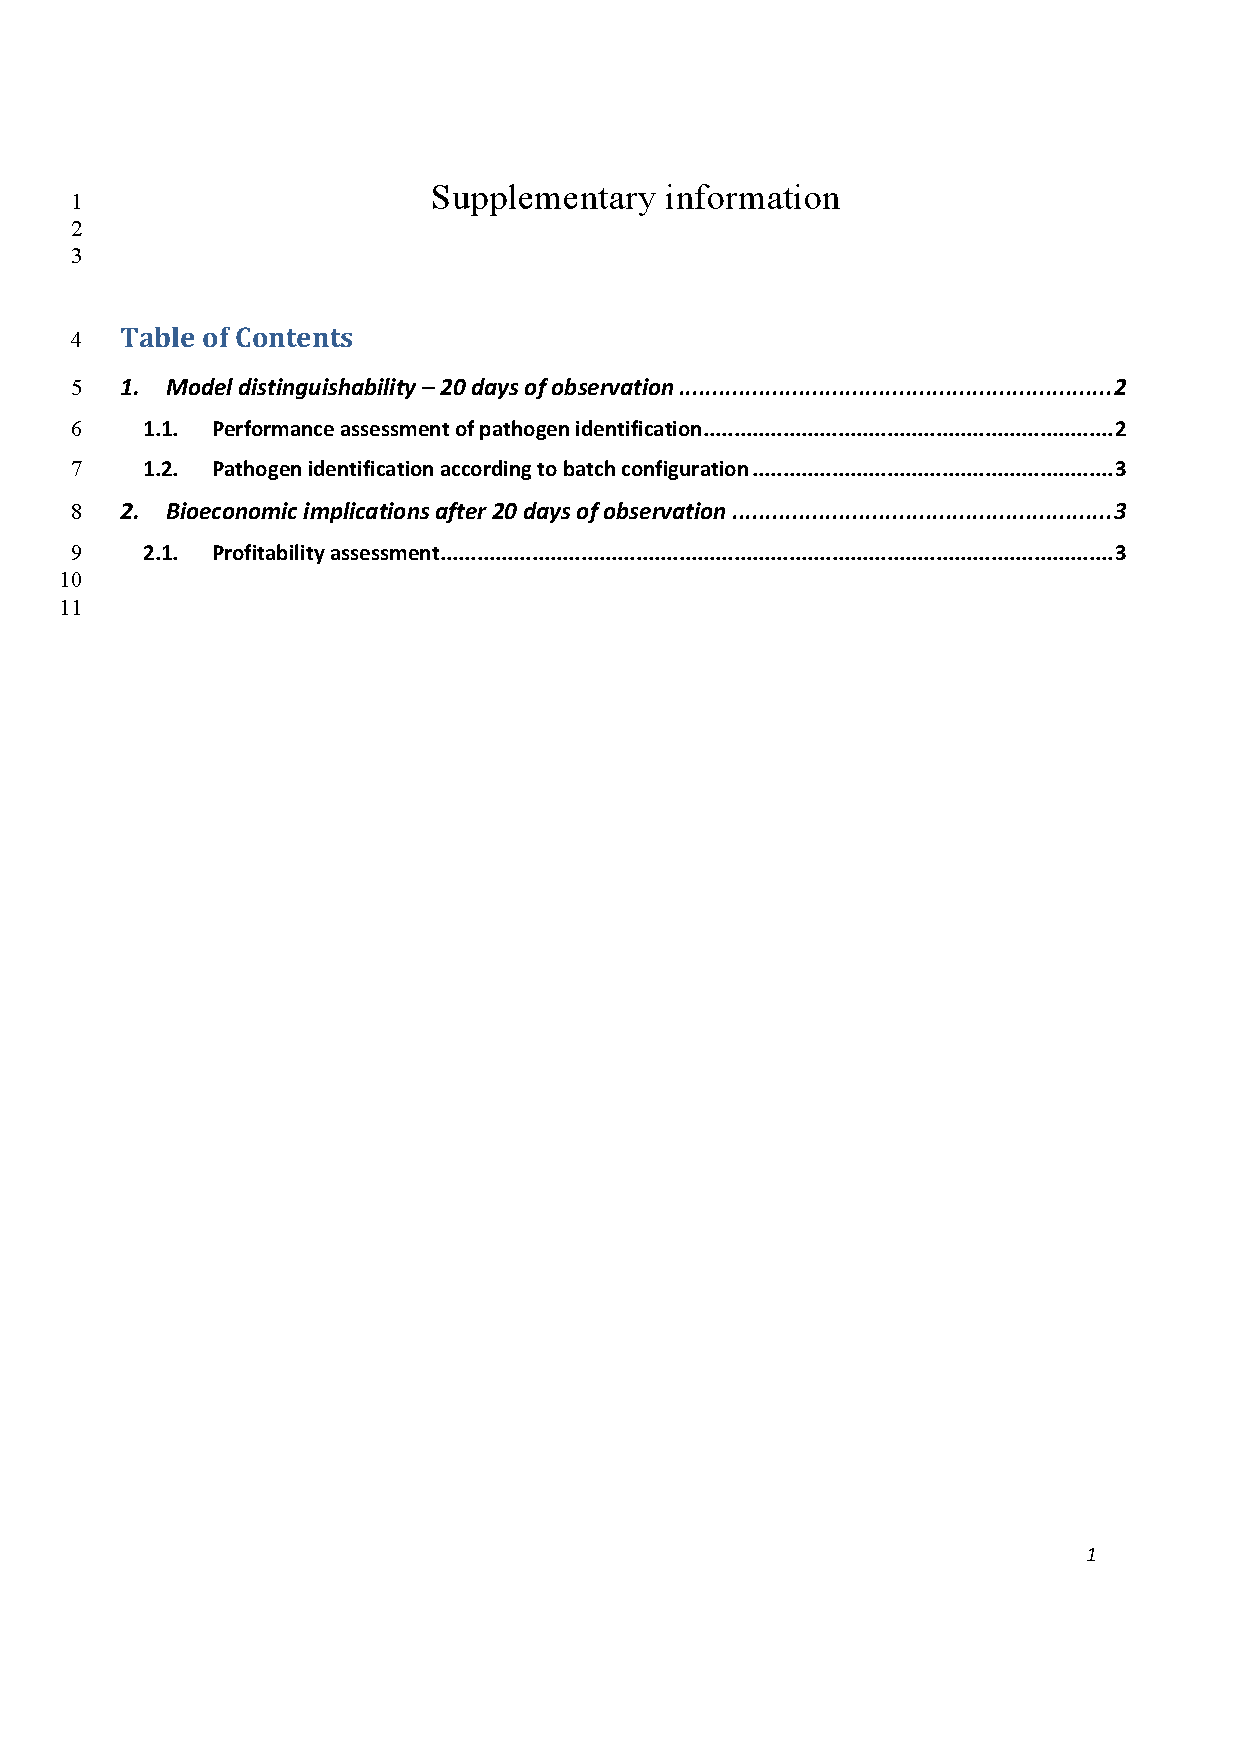
\includepdf[pages=-]{articles/supp-mat3.pdf}

% \chapter*{\Huge Big Title Here}
% \addcontentsline{toc}{chapter}{Big Title Here}  % Add to TOC if needed

% \chapter{Components integration - a deep mechanistic approach} % propositions de titre
\chapter{A deep mechanistic model: Grounded mechanistic model for adaptive knowledge}
%----------------------------------------------------------------------------------------
%	SECTION 
%----------------------------------------------------------------------------------------
\section{Introduction}
%-----------%-----------
%	SOUS-SECTION 
%-----------%-----------

 % pour justifier la précision obtenue: Moreover, for BRD and similar conditions there is no universally accepted “gold standard” diagnostic: clinical thresholds vary by practitioner and farm context, and standard laboratory tests (e.g., bacterial culture) can take days to return, further compounding uncertainty in disease classification

\subsection{Contextual background}
Modern sensor modalities (e.g., lung ultrasound, video and audio surveillance, etc) offer high‑frequency, objective measurements that overcome many limitations of human observation (inter‑observer variability, delayed reporting). However, these measurements represent only the observable manifestations of underlying pathophysiological processes and thus provide an incomplete, noisy “snapshot” of disease state—what Yoan Bourhis (2017) aptly describes as the “tip of the iceberg” .

Aleatoric uncertainty refers to the inherent noise and variability present in the data itself. In the context of sensor‑based diagnostics—such as lung ultrasound videos of cattle, aleatoric uncertainty arises from factors beyond the model’s control: image acquisition artifacts, animal movement, inconsistent probe positioning, and intrinsic biological variability in disease presentation. Because aleatoric uncertainty reflects randomness in the observation process, it cannot be reduced simply by collecting more data; instead, it must be explicitly modelled so that downstream predictions correctly reflect the limits of information contained in each measurement. Epistemic uncertainty, by contrast, captures the model’s lack of knowledge about the correct mapping from inputs to outputs. This form of uncertainty is highest when the model encounters examples that are far from the distribution of its training data—rare clinical presentations, novel farm environments, or unforeseen sensor configurations. Unlike aleatoric uncertainty, epistemic uncertainty can be reduced through the acquisition of additional, representative training examples. Crucially, a model can output a high softmax score (traditional logits interpreted as probabilities) even when its epistemic uncertainty is large, leading to overconfident and potentially erroneous predictions \cite{gal_dropout_2016}.

Epidemiological forecasting relies on mechanistic models, which codify known biological relationships (transmission rates, immune response kinetics, within‑host pathogen dynamics) into mathematically tractable systems of equations. While these models capture long‑term disease trajectories and can simulate the effects of interventions at the population level, they are poorly informed by sensor data when observations are unstructured, sparse and noisy.


% Standard deep‑learning pipelines commonly equate the softmax output of the final layer with predictive confidence, yet this conflation masks both aleatoric and epistemic uncertainties and gives no indication of when a prediction should be trusted. In high‑stakes veterinary diagnostics, such overconfidence can result in inappropriate treatments, delayed intervention, and significant economic and welfare costs.


%-----------%-----------
%	SOUS-SECTION 
%-----------%-----------
\subsection{Article Originality and objectives}

\paragraph{To what extent can automated short-term diagnostics derived from limited sensor observations effectively inform and specify a mechanistic epidemiological model for long-term disease prognosis?} In this work, we propose and explore a novel hybrid methodology explicitly aimed at integrating deep learning, sensor-based diagnostics with a mechanistic epidemiological model (Fig \ref{fig:chap4-question1}). Specifically, we develop an approach that leverages short-term, sensor-derived diagnostics obtained from limited Lung Ultrasound (LUS) video data to inform parameter calibration in epidemiological models. We employ a Bayesian Deep Mechanistic approach to bridge sensor-based diagnostics and mechanistic forecasting. This integration aims to enhance the interpretability, and practical applicability of epidemiological prognosis, enabling accurate long-term disease management strategies from inherently limited and uncertain short-term observations. 


\begin{figure}[H]
  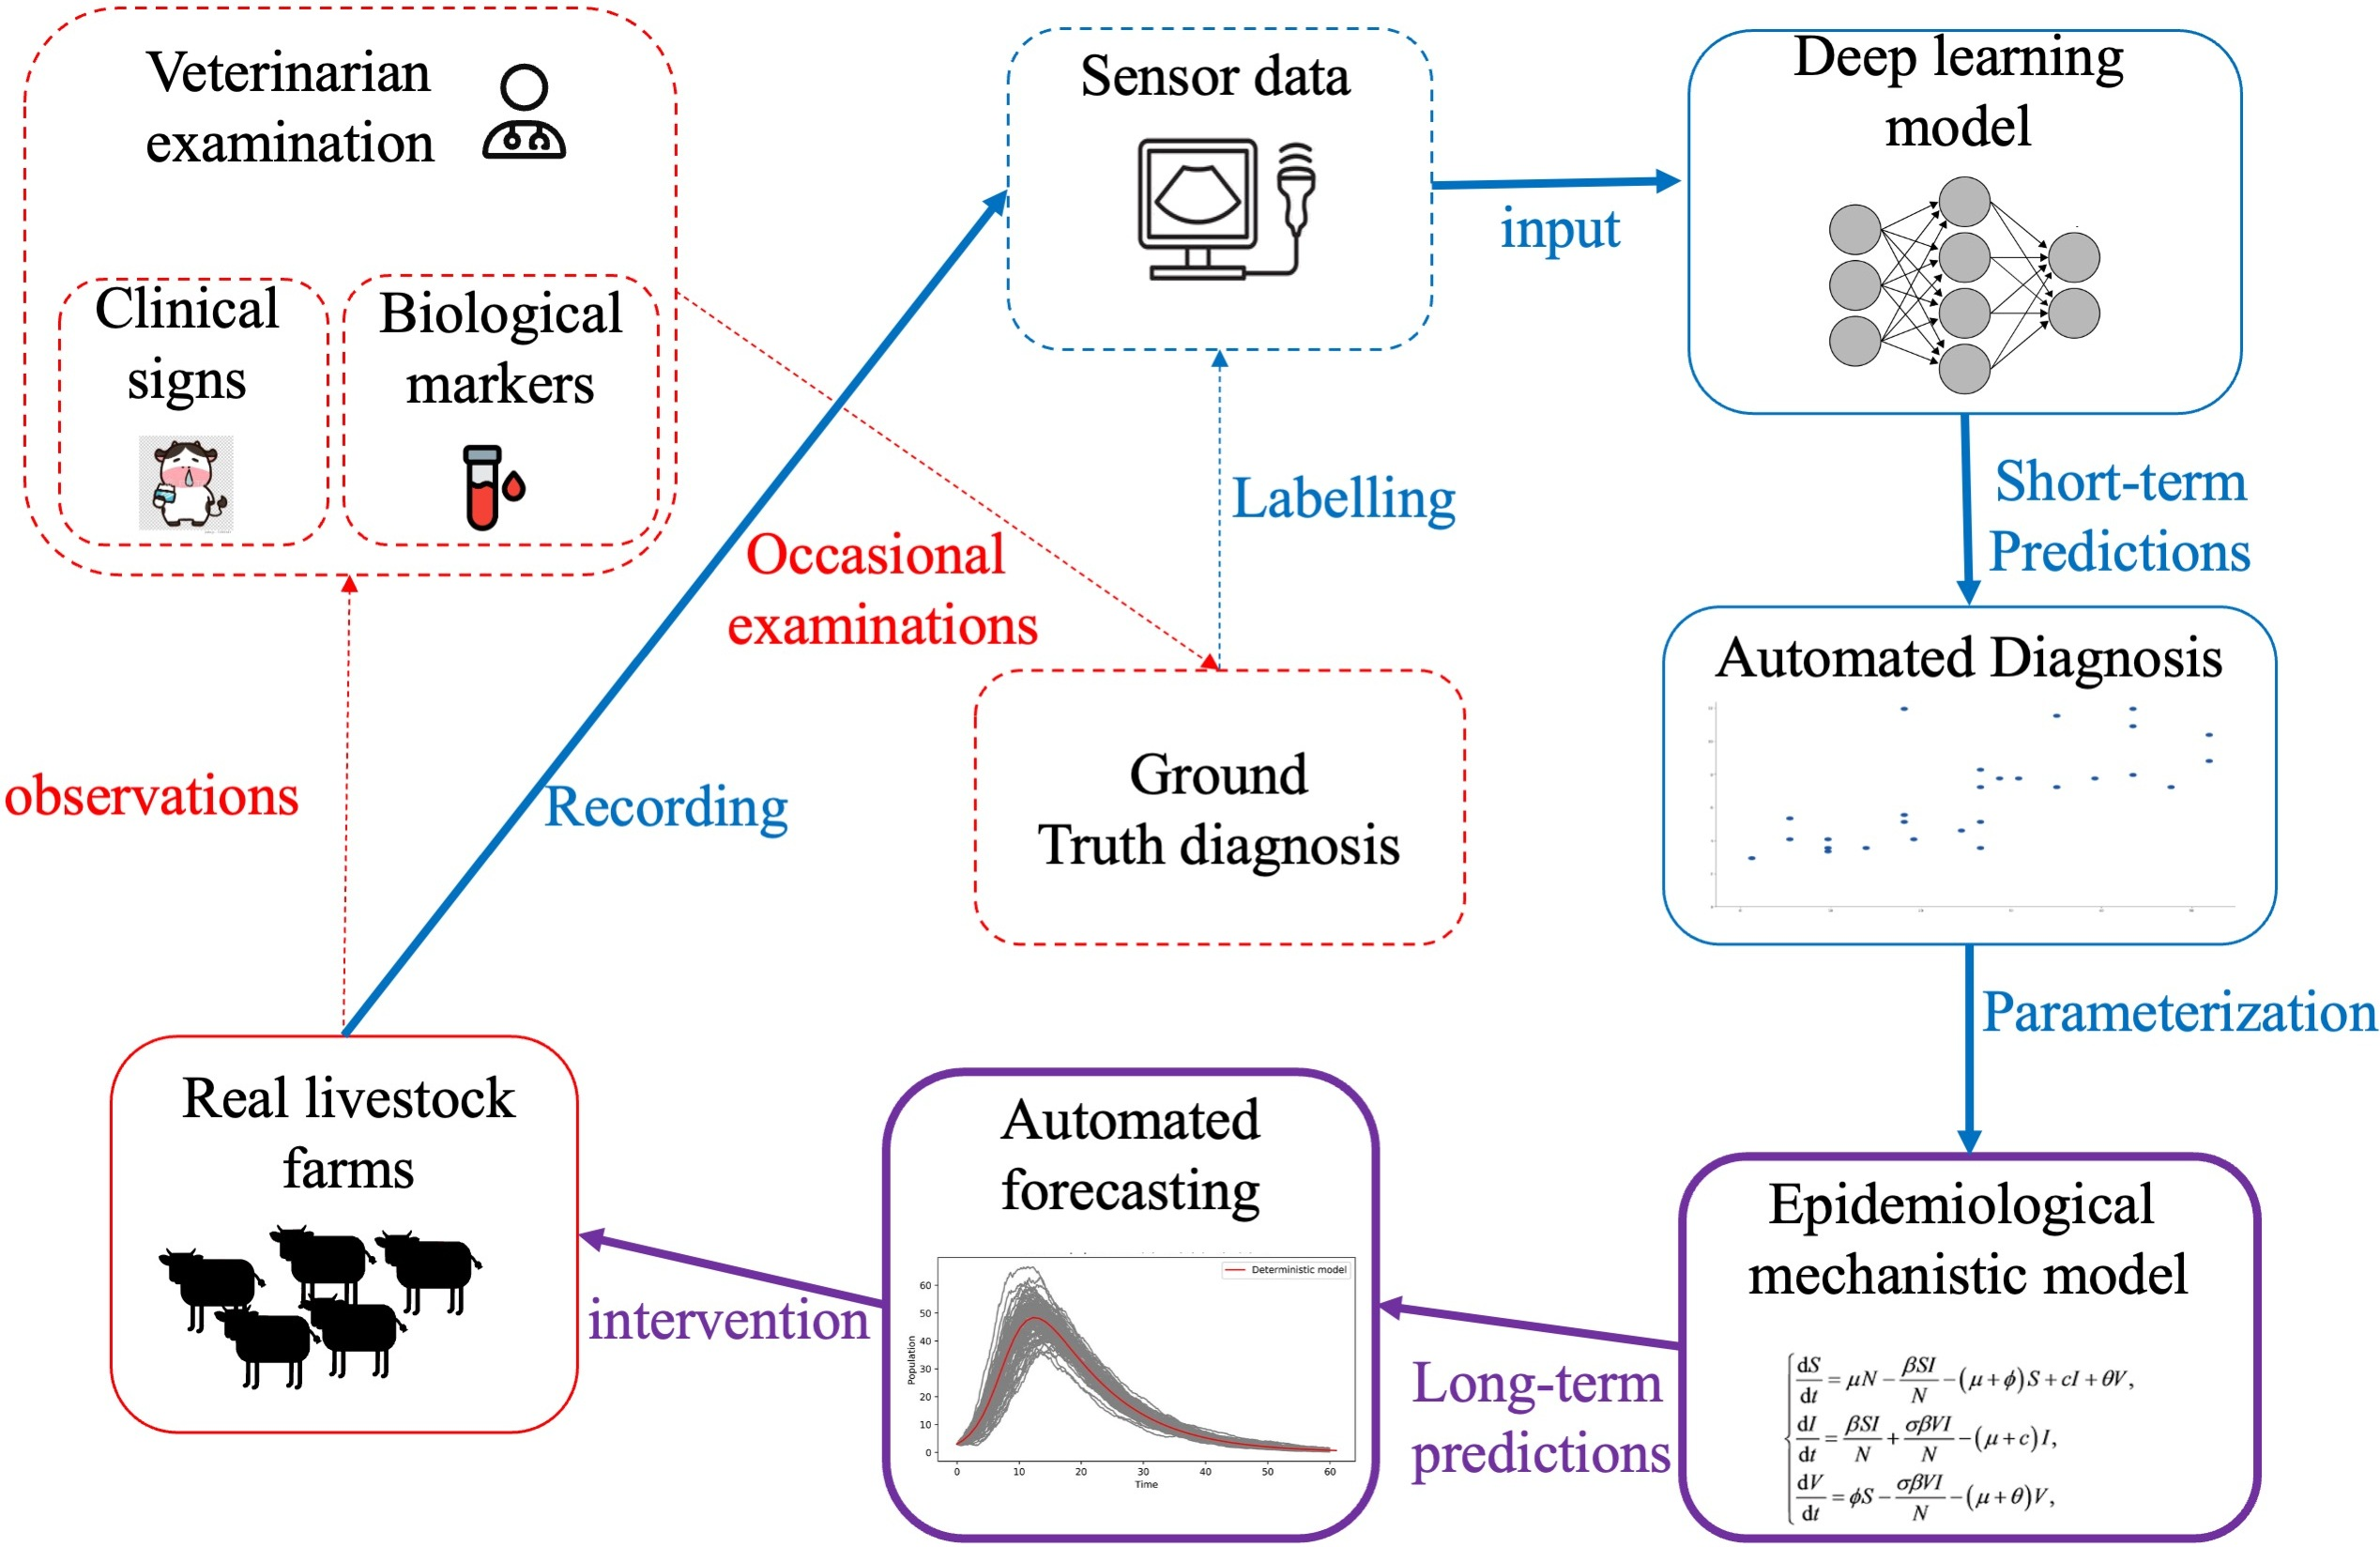
\includegraphics[width=\linewidth]{figures/chap4/chap4-question1.jpg}
  \caption{Sketch workflow of a ...}
  \label{fig:chap4-question1}
\end{figure}

\paragraph{How can intrinsic uncertainties inherent in sensor-derived diagnostic data, especially noisy observations such as Lung Ultrasound (LUS) videos, be explicitly quantified and incorporated into mechanistic models to ensure a more robust and trustworthy prognostic prediction ?}

Given the intrinsic uncertainty and noisiness of real-world LUS videos, exacerbated by animal movement and image acquisition limitations, this work explicitly addresses the quantification and integration of these uncertainties into the diagnostic and prognostic pipeline. We variational methods in Bayesian deep learning model to quantify the uncertainty associated with sensor-based diagnostic predictions. Bayesian probability theory offers us mathematically grounded tools to reason about model uncertainty. These quantified uncertainties are subsequently managed through two complementary approaches: either by filtering out high-uncertainty, unreliable observations (Out-of-distribution detection) to ensure safe prognosis and prioritize them for detailed veterinary reassessment, or by directly propagating uncertainties into mechanistic model calibration through uncertainty-weighted parameter inference. This dual strategy enhances the robustness, reliability, and practical applicability of long-term prognostic predictions.


%-----------%-----------
%	SOUS-SECTION 
%-----------%-----------
\subsection{Main contributions}
This chapter introduces the Bayesian Deep Mechanistic (BDM) model, a novel integrative approach that leverages both data-driven diagnostics derived from sensor technologies and knowledge-driven epidemiological modeling. This integration addresses critical limitations inherent in existing diagnostic and prognostic methodologies, specifically for Bovine Respiratory Disease (BRD), by explicitly quantifying and managing uncertainty from limited and noisy sensor observations. Three main contributions emerge from the approach presented in this chapter:


\begin{enumerate}
    \item \textbf{Coupling punctual diagnostics with mechanistic forecasting (fig \ref{fig:chap4-method1}).}   We designed and trained a hybrid deep learning pipeline, a spatio-temporal CNN‑RNN—that ingests raw lung ultrasound (LUS) video clips and outputs a binary infectious status (infectious vs. non‑infectious) for individual bovine. Our dataset comprised 265 LUS videos collected from 163 animals across nine French farms, capturing real‑world variability in lesion appearance, probe positioning, and animal movement.  Crucially, these “punctual” diagnostic predictions served not only as standalone classifiers but also as the empirical anchor for calibrating a mechanistic epidemiological model via Approximate Bayesian Computation (ABC). In practice, we treat each deep learning prediction as a point estimate of batch‑level infection prevalence at discrete observation times; ABC then infers the three key parameters—initial prevalence, average infectious duration, and transmission rate—that best reconcile the mechanistic model’s simulated infection trajectories with these sensor‑derived snapshots. This coupling bridges short‑term, deep learning diagnostics and long‑term, mechanistic forecasts. 

    Although fully automated and practical for on‑farm use, our diagnostic model achieved a relative root‑mean‑square error (RRMSE) of 39\% against veterinarian‑confirmed labels, reflecting the inherent noise and variability of LUS data. When these predictions alone were used to parametrize the mechanistic model, the resulting 30‑day forecast exhibited an RRMSE of 38.4\%, substantially higher than the 23\% error attained when using veterinarian ground‑truth diagnostics. This gap underscores both the promise of automated sensing for scalable disease surveillance and the imperative of explicitly quantifying and managing uncertainty in order to approach the accuracy of expert‑driven prognostics.

    \begin{figure}[H]
      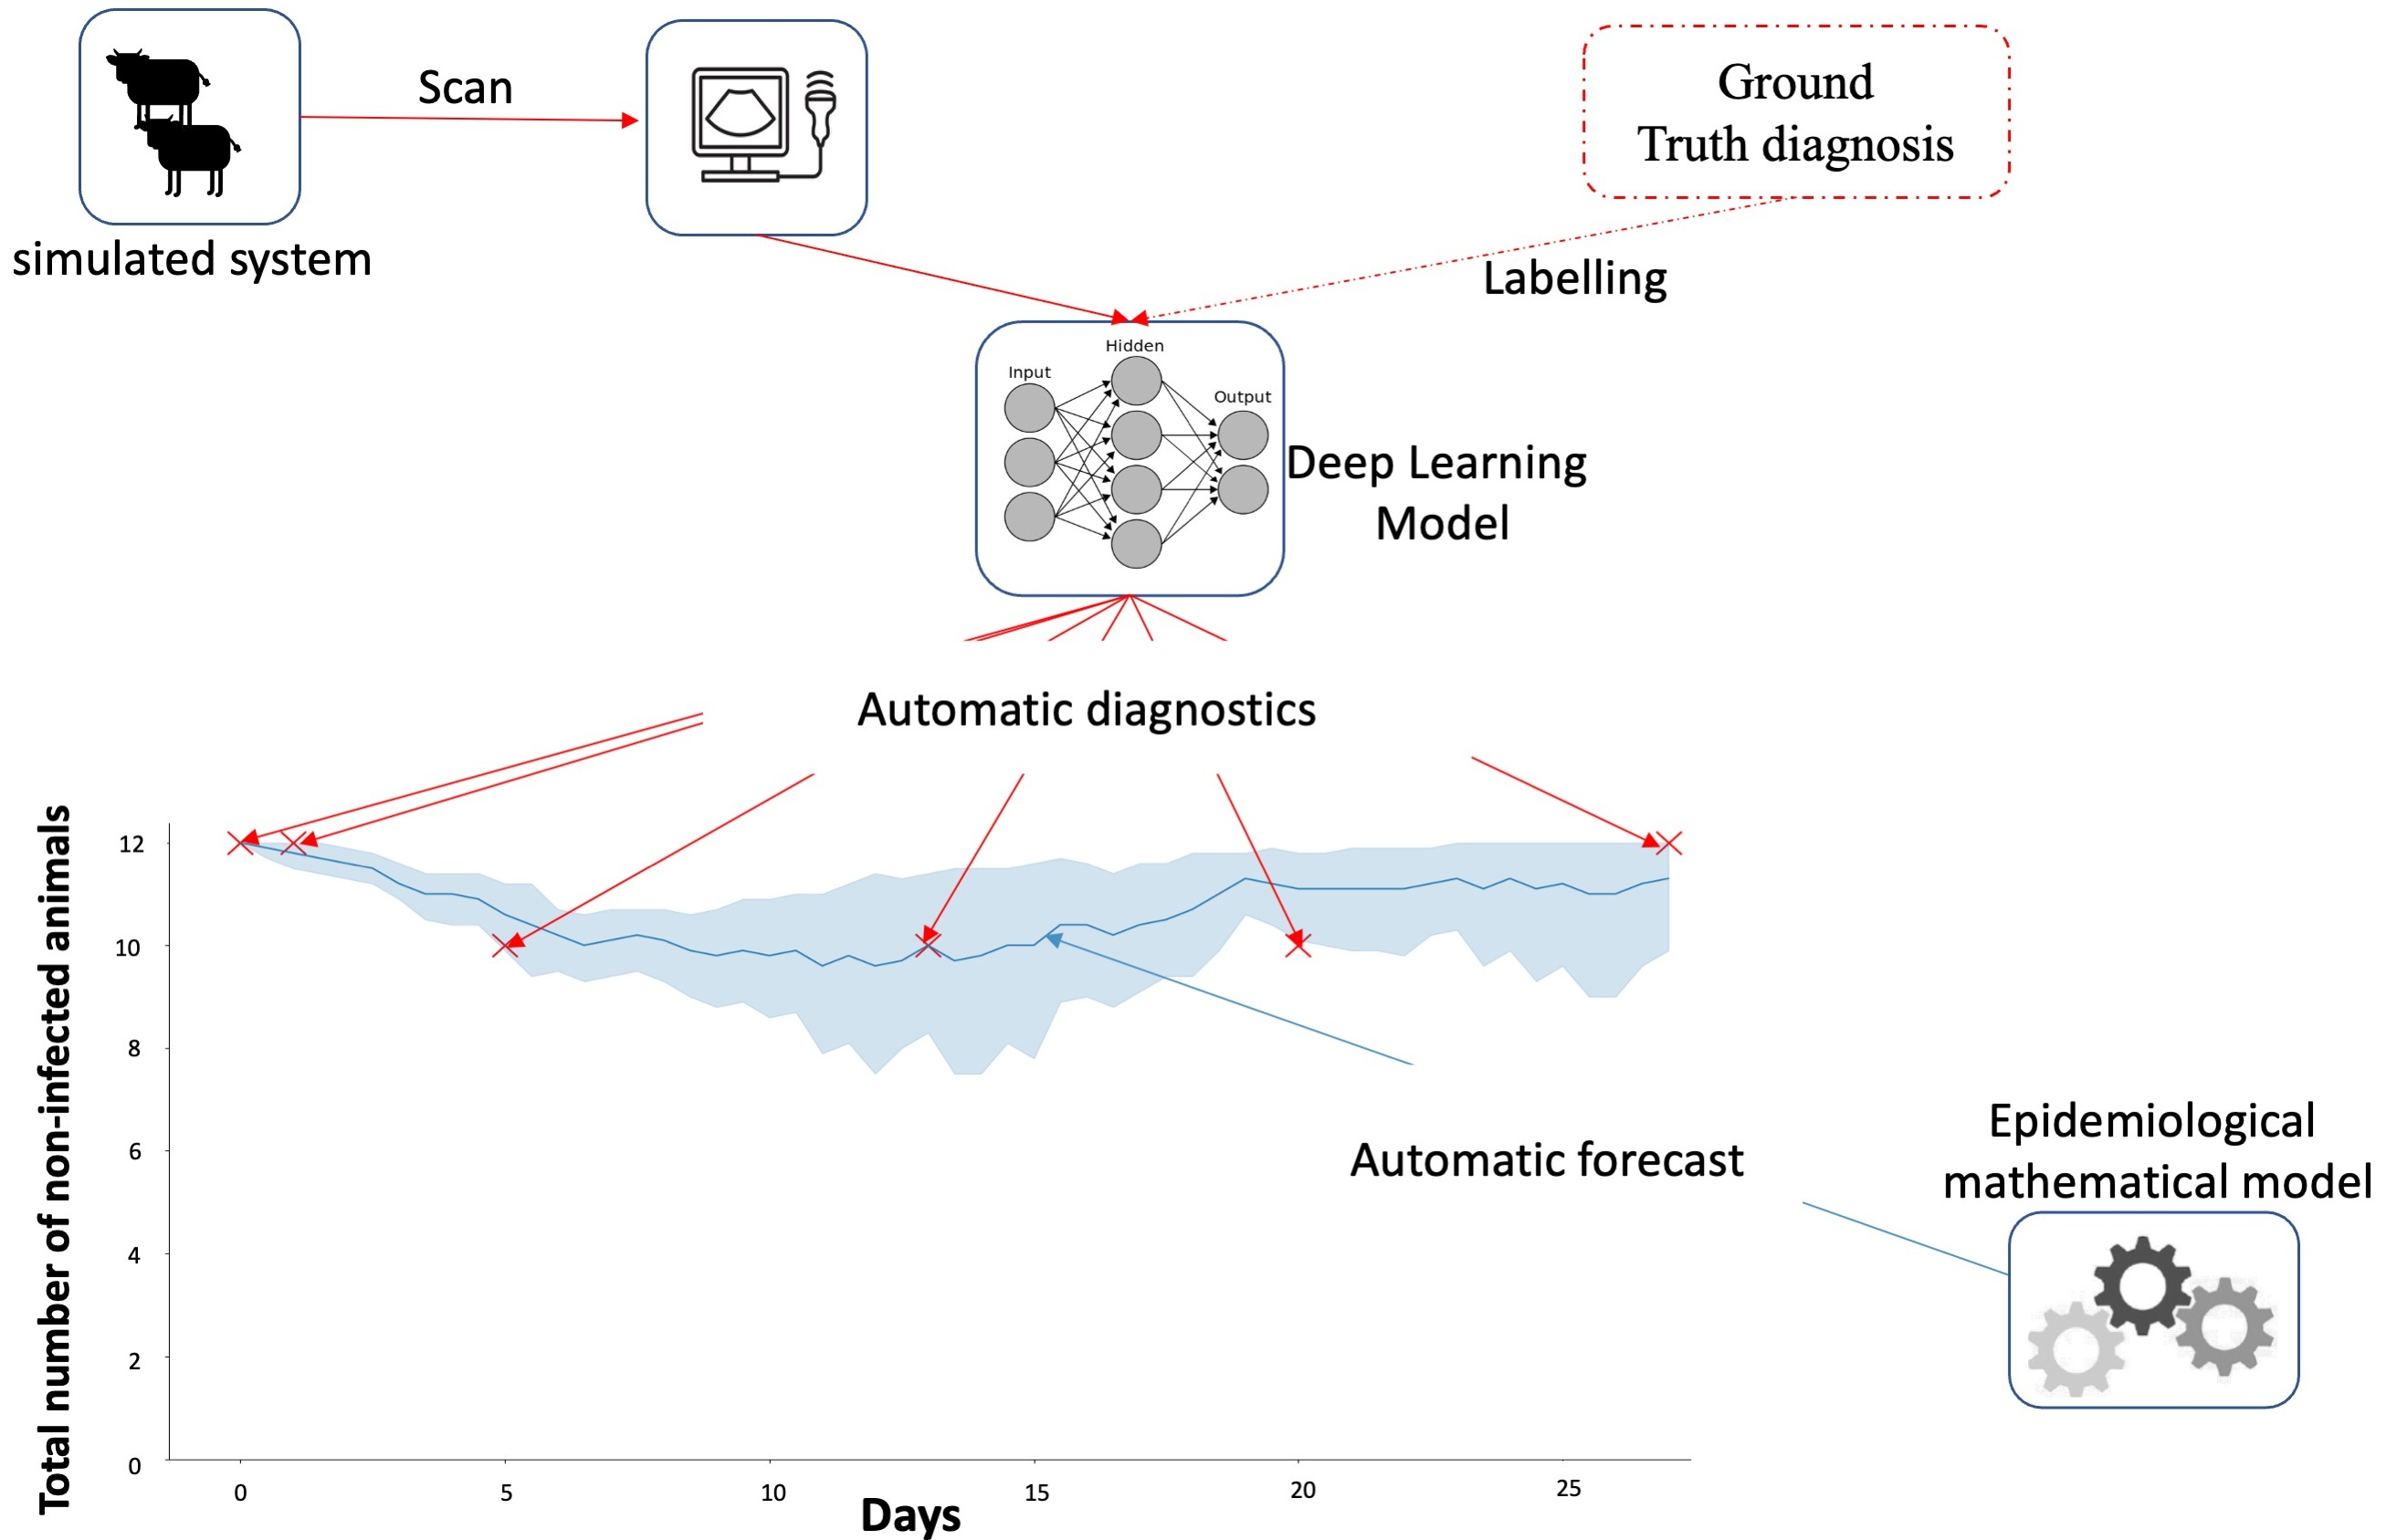
\includegraphics[width=\linewidth]{figures/chap4/method 1.jpg}
      \caption{coupling punctual diagnostics with mechanistic forecasting}
      \label{fig:chap4-method1}
    \end{figure}

    \item \textbf{Sensor observation cleansing through Uncertainty-Based Filtering (fig \ref{fig:chap4-method2}).} Lung ultrasound (LUS) videos are full with sources of noise, animal motion, suboptimal probe positioning, uninterpretable image artifacts—that can lead a deterministic classifier to make confidently wrong predictions (In chapter 1 \ref{fig:chap2-question1},  we achieved only a 72\% accuracy, for a binary classifier, that is low). In order to control this risk in observations used, we had to explicitly capture the epistemic uncertainty (i.e., the model’s lack of knowledge). For that we converted our CNN‑RNN DL model into a Bayesian deep learning model using Monte Carlo Dropout (MCD). During inference, MCD performs dozens of stochastic forward passes with dropout active, producing a distribution of softmax probability vectors rather than a single point estimate. We then quantify uncertainty by computing the Shannon entropy of each video’s averaged class probability distribution—a well‑established acquisition function in active learning that measures the spread (disorder) of predictive beliefs. High entropy indicates low confidence and signals inputs for which the model’s knowledge is insufficient.

    By ranking predictions by entropy, we implemented an uncertainty‑based filter: low‑entropy (high‑confidence) cases are accepted as automatic diagnoses, while high‑entropy (low‑confidence) cases are flagged for veterinarian review. This selective acceptance dramatically improved diagnostic accuracy, lowering the relative root‑mean‑square error (RRMSE) from 39\% (deterministic predictions) to 32\% against veterinarian ground truth. Crucially, when only filtered (high‑confidence) diagnoses were used to calibrate our epidemiological model, the 30‑day forecast error fell to 27.2\% RRMSE—much closer to the 23\% error achieved using full veterinarian diagnoses
    
        \begin{figure}[H]
          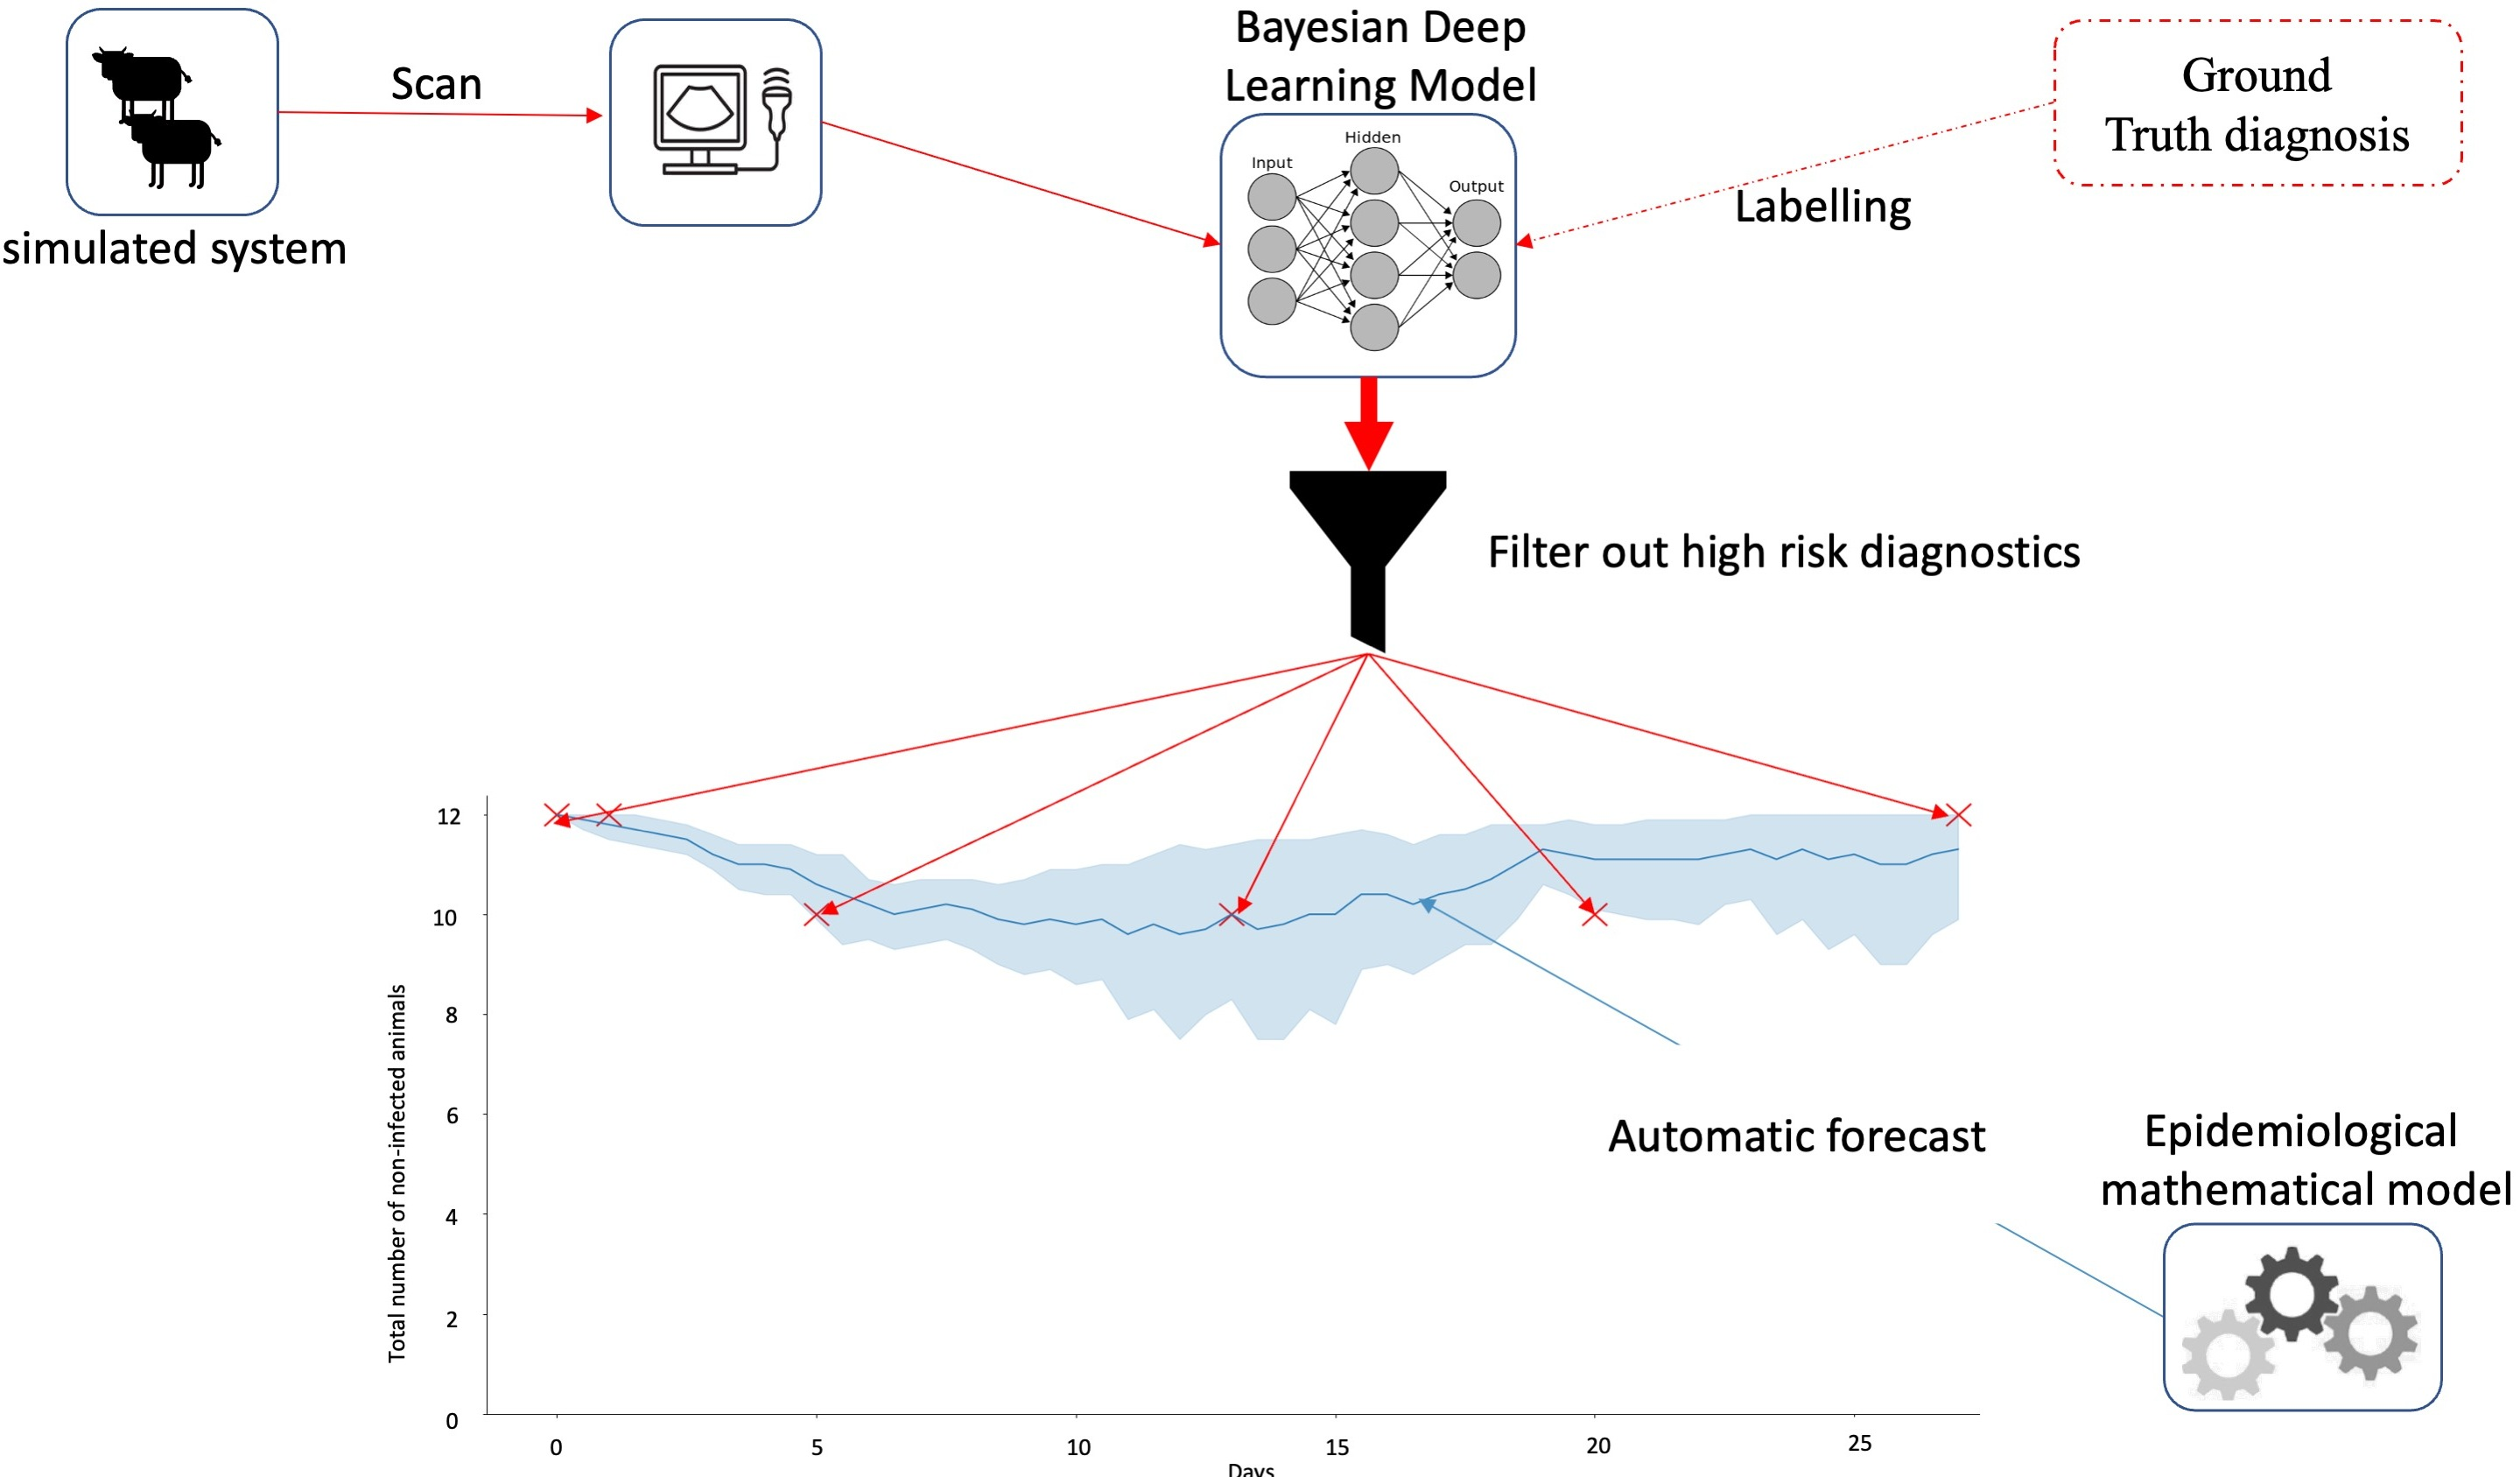
\includegraphics[width=\linewidth]{figures/chap4/method 2.jpg}
          \caption{Sensor observation cleansing through Uncertainty-Based Filtering}
          \label{fig:chap4-method2}
        \end{figure}

    \item \textbf{Prognosis robustness through Uncertainty Propagation (fig \ref{fig:chap4-method3}).} Rather than discarding low‑confidence diagnoses, we leveraged each prediction’s quantified uncertainty to inform the parametrization of a stochastic mechanistic epidemiological model. After obtaining a posterior distribution (uncertainties) over batch‑level infectious counts via Monte Carlo Dropout, we extracted both the mean (as the point estimate of infected prevalence) and its variance (as a measure of diagnostic confidence). During Approximate Bayesian Computation (ABC) parameter inference, we replaced the standard Euclidean distance with a weighted version in which each observation’s contribution was inversely proportional to its uncertainty (i.e., higher variance → lower weight). This uncertainty‑weighted inference ensures that reliable, low‑variance diagnostics exert greater influence on parameter estimation (pathogen transmission rate, mean duration in the infectious state, mean duration in the pre-infectious state), while noisy, high‑variance observations contribute less, effectively down-weighting potentially misleading observations rather than excluding it outright. The result is a more robust posterior over epidemiological parameters and, consequently, more accurate long‑term forecasts: the uncertainty‑propagated model achieved a 30‑day forecast RRMSE of 27.2\% nearly matching the 23\% error obtained when calibrating solely on veterinarian‑confirmed diagnoses. This method also reduces diagnostic error from the deterministic model’s 39\% RRMSE to 32\% RRMSE, matching the improvement seen in our uncertainty‑filtering approach

    These results demonstrate that explicitly propagating diagnostic uncertainty not only improves automated classification but also closes most of the remaining gap between sensor‑based forecasts and expert‑driven prognostics, unlocking robust long‑term predictions from inherently noisy, limited observations. By embedding predictive uncertainty directly into the model calibration process, our approach preserves information from all sensor‑based observations maximizing data utility, while mitigating the impact of noise.

    \begin{figure}[H]
      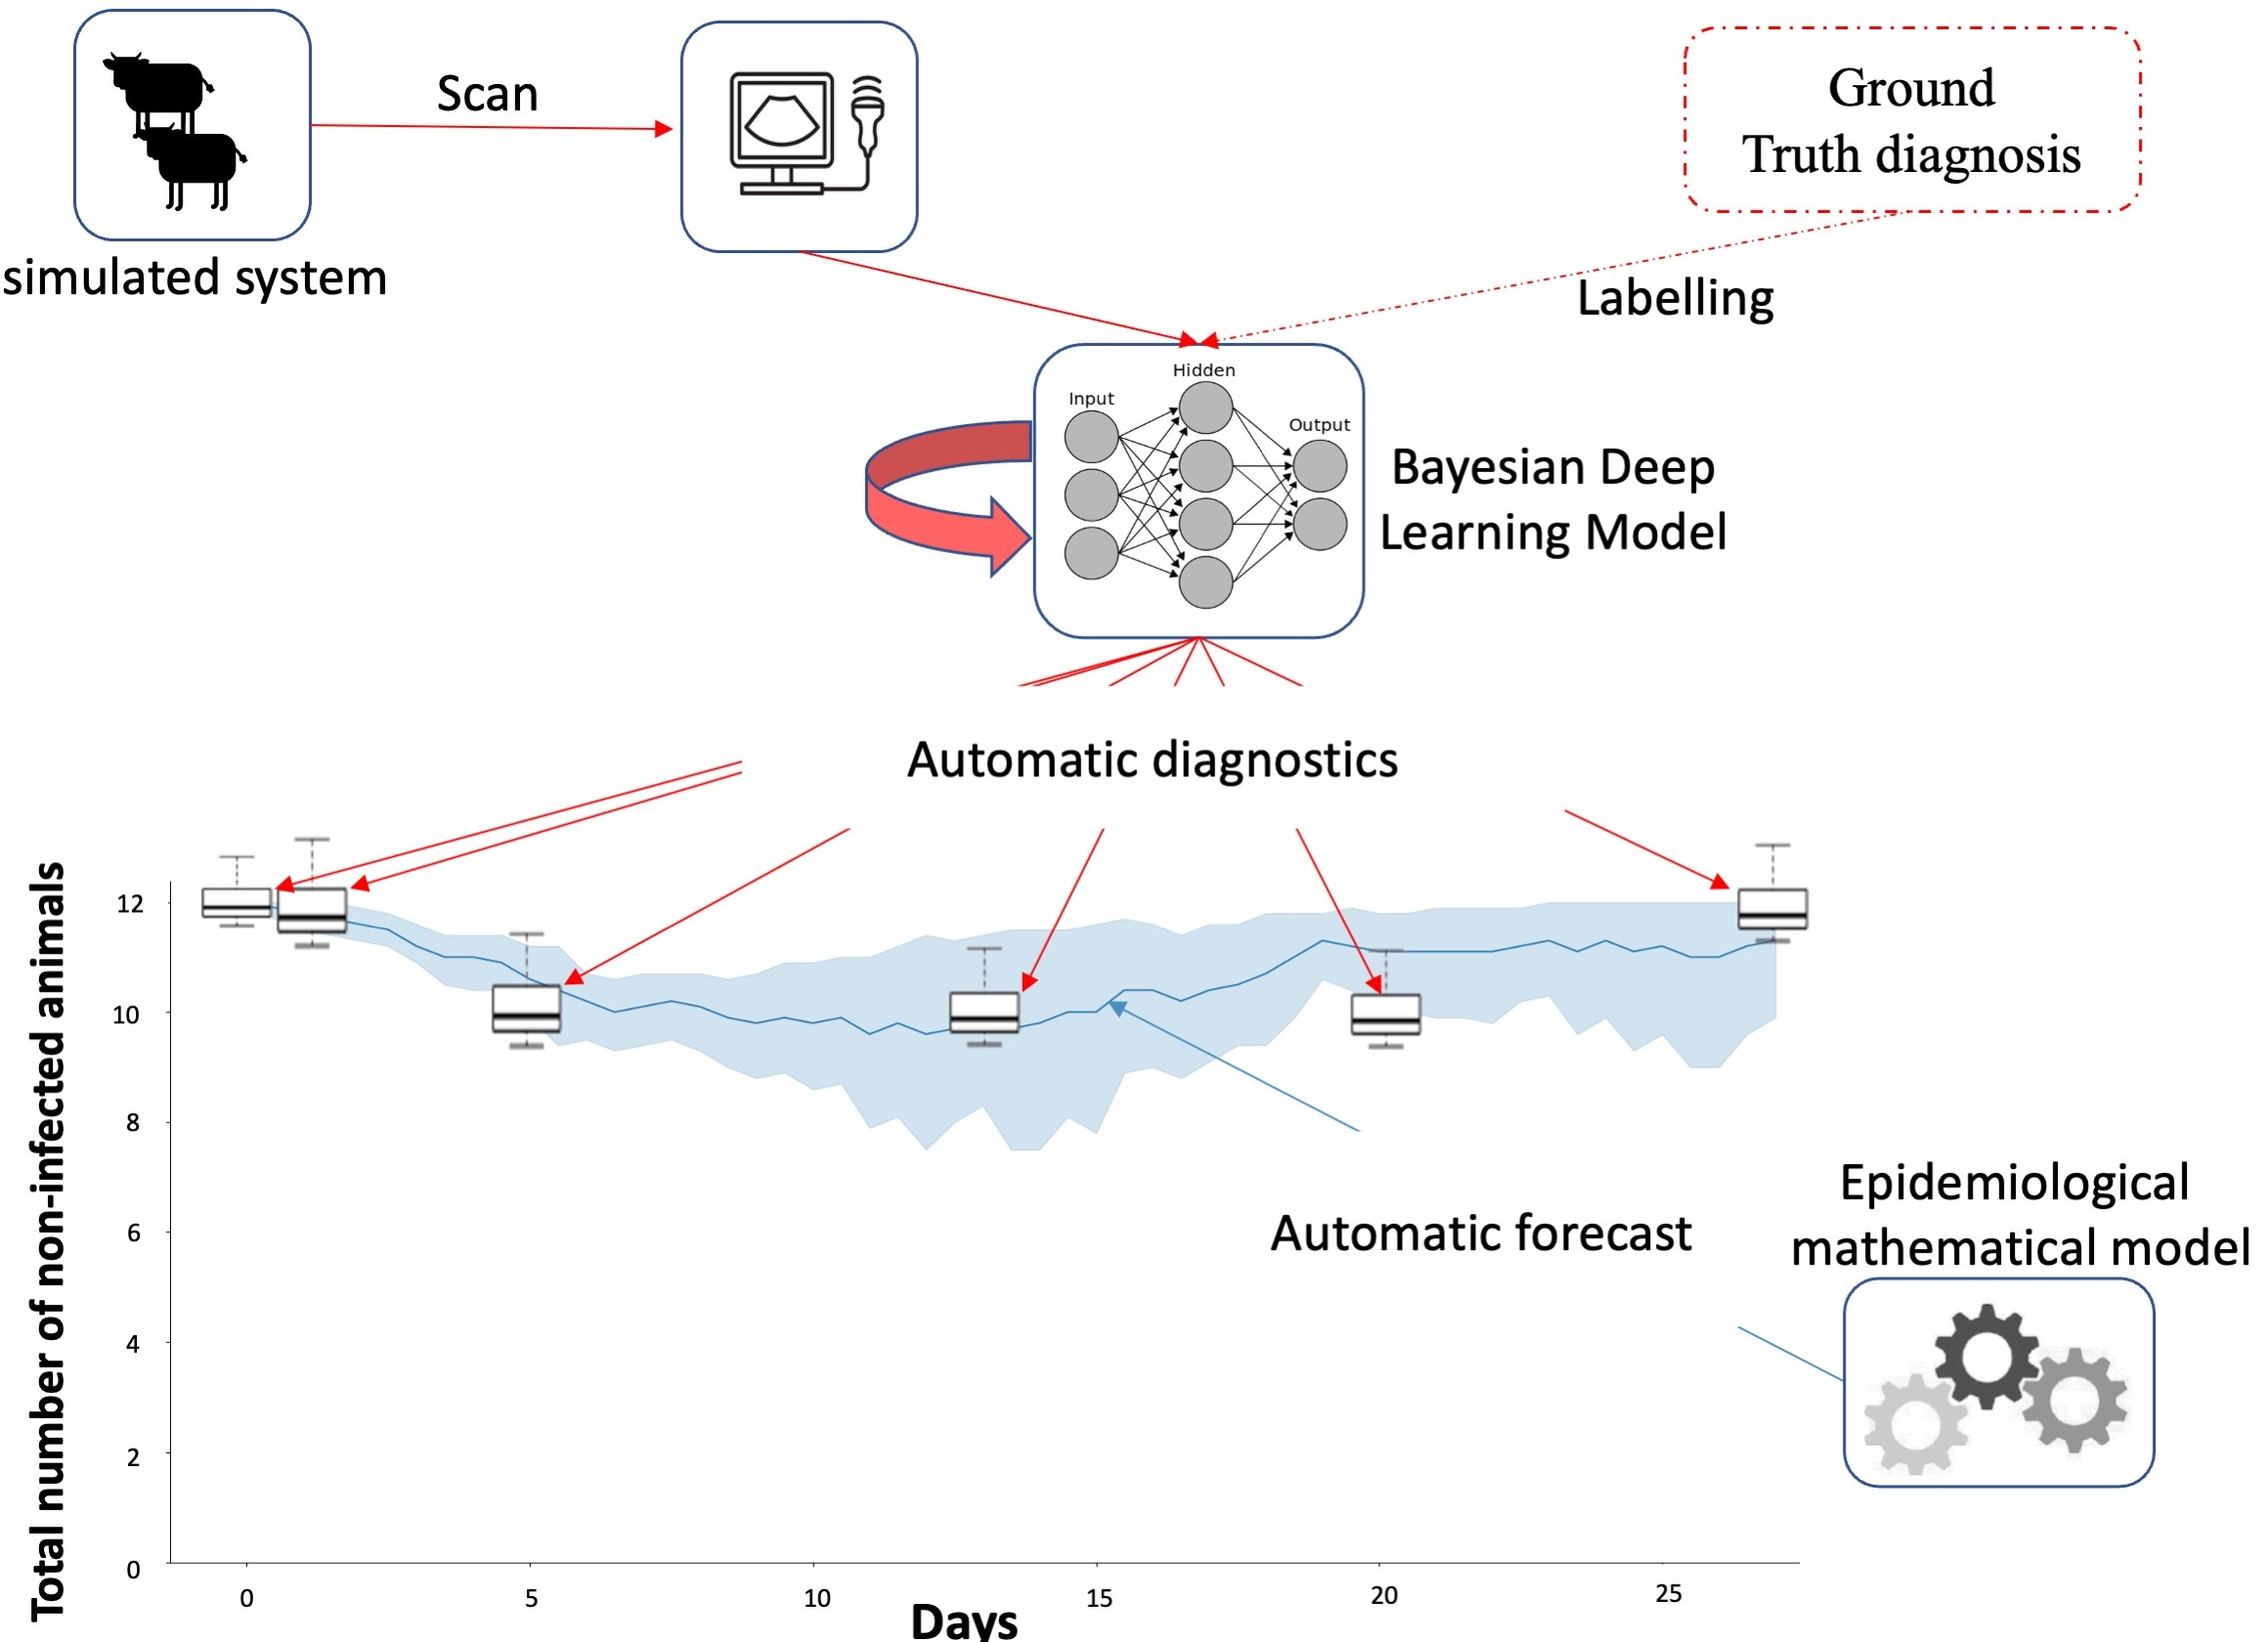
\includegraphics[width=\linewidth]{figures/chap4/method 3.jpg}
      \caption{Prognosis robustness through Uncertainty Propagation}
      \label{fig:chap4-method3}
    \end{figure}
    
\end{enumerate}

 
\subsection{[In French] Résumé grand public} 

La santé animale et la prévention des maladies infectieuses reposent de plus en plus sur des technologies de diagnostic automatisées, comme l’échographie pulmonaire chez les bovins. Toutefois, ces données issues de capteurs sont souvent bruyantes, incomplètes et sujettes à des erreurs d’interprétation. Notre étude propose une nouvelle approche hybride qui combine l’intelligence artificielle (IA) et les modèles mathématiques traditionnels (appelés «mécanistiques») pour améliorer la détection précoce et la prévision à long terme de la maladie respiratoire bovine.

Nous avons d’abord développé un modèle d’apprentissage profond capable d’analyser automatiquement de courtes vidéos d’échographie pulmonaire et de prédire si un animal est infectieux ou non. Pour tenir compte de l’incertitude inhérente à ces diagnostics automatisés (problèmes de qualité d’image, mouvements de l’animal…), nous utilisons une technique bayésienne qui mesure la confiance de chaque prédiction. Les cas où le modèle est peu sûr sont soit signalés pour un examen vétérinaire, soit pondérés de façon moindre dans les étapes suivantes.

Ensuite, ces diagnostics ponctuels, enrichis de leur degré de confiance, servent à calibrer un modèle épidémiologique mathématique qui simule la propagation de la maladie dans un troupeau sur plusieurs semaines. Cette intégration («fusion») permet de produire des prévisions de l’évolution de l’infection plus fiables que celles basées uniquement sur l’IA ou uniquement sur les modèles traditionnels. Concrètement, notre méthode réduit l’erreur de prédiction à 27\% sur 30 jours — un résultat proche de la précision obtenue lorsqu’on utilise exclusivement des diagnostics vétérinaires, mais avec un processus entièrement automatisé et évolutif pour une utilisation directe en élevage.

En résumé, cette étude démontre qu’il est possible d’exploiter efficacement des données de capteurs imparfaites grâce à une modélisation hybride : l’intelligence artificielle apporte une analyse rapide et à grande échelle, tandis que le modèle mathématique garantit une prévision robuste à long terme. Cette approche ouvre la voie à une surveillance de la santé animale plus précise, proactive et accessible, contribuant à améliorer le bien‑être des animaux et à réduire les pertes économiques liées aux maladies infectieuses.


\section{Article published in Preventive Veterinary Medicine (Elsevier), 2024}


    % \input{chapters/chap1-article} # pas besoin de mettre un file appart sauf si j'ai des choses spécifiques à rajouter pour cette partie
    \includepdf[pages=-]{articles/PVM.pdf}  % Replace with your actual filename



%\part*{Discussion et conclusion générale}
\fancyhead{} % clear all header fields
\fancyhead[OL]{\textsc{General discussion}}
% \chapter*{\Huge Big Title Here}
% \addcontentsline{toc}{chapter}{Big Title Here}  % Add to TOC if needed

\chapter{General discussion} % Main chapter title


%----------------------------------------------------------------------------------------
%	SECTION 
%----------------------------------------------------------------------------------------
\section{Main contributions}
%-----------%-----------
%	SOUS-SECTION 
%-----------%-----------

\subsection{Methodological progress}

\paragraph{Integration of sensor-based and mechanistic models} A central methodological advancement of this thesis lies in the integration of deep learning diagnostic tools and mechanistic epidemiological models for improved disease management, specifically applied to the Bovine Respiratory Disease (BRD) context. This thesis explicitly addressed the complexities inherent in integrating disparate model types, reconciling sensor-driven, short-term diagnostic accuracy with long-term epidemiological prognosis reliability. Inspired by the "Mixture of Experts" (MoE) concept, our methodology systematically separates diagnostic and prognostic tasks, assigning each model type to its respective domain of expertise. This loose coupling has two main methodological strengths:

\begin{enumerate}
    \item Diagnostic specialization: Deep learning excels at extracting timely and accurate diagnostic insights from sensor observations, even under conditions of limited and noisy data (72\% accuracy with less than 30 lung ultrasound videos). This demonstrated capability supports practical, short-term veterinary decision-making by automating complex clinical assessments that otherwise require significant veterinary expertise and resources. Remarques: [est-ce grave de n'avoir "que" 72\% de précision ? -> limitation à discuter]
    
    \item Prognostic specialization: Mechanistic epidemiological models reliably extend diagnostic insights into accurate, long-term disease forecasts. Calibrating these models using empirical veterinary observations resulted in robust epidemiological predictions (forecast accuracy RMSE < 10\%), demonstrating their value for long-term disease management and strategic decision-making.
\end{enumerate}

\paragraph{Explicit integration and propagation of uncertainty} One of the essential questions addressed in this thesis concerns uncertainty management: How to explicitly handle uncertainty inherent in sensor-based observational data within hybrid diagnostic-prognostic models? This question is especially relevant for BRD diagnostics, given the inherent complexity and ambiguity of symptoms, compounded by noisy and limited ultrasound data acquisition.
To explicitly manage uncertainty, we introduced a Bayesian Deep Mechanistic approach where uncertainty quantification via Monte Carlo Dropout (MCD) played a pivotal role. We quantified prediction uncertainty at the diagnostic level, filtering out the most uncertain predictions and consequently reducing diagnostic error rates from an initial RRMSE of 39\% down to 32\%. Additionally, propagating these uncertainties into mechanistic model calibration, via weighted Approximate Bayesian Computation, further improved the prognosis reliability, achieving a forecast RRMSE of 27.2\%, nearly matching the veterinarian-informed baseline (23\% RRMSE).

Our proposed solution is interesting because it directly confronts the real-world complexities of sensor-driven observations, integrating probabilistic quantification of uncertainty into the predictive decision-making pipeline. This ensures robust diagnosis and prognosis even in scenarios where data quality is inherently compromised or limited, a frequent reality in livestock management practices.

Remarques: [à développer, notamment en expliquant plus en détail "pourquoi ça marche" et l'articulation entre prédiction ML et prédiction méca]

\paragraph{Pathogen identification through mechanistic model distinguishability} A significant methodological innovation introduced in this thesis was the pathogen-specific mechanistic model identification using Approximate Bayesian Computation (ABC) combined with multinomial logistic regression. By employing symptomatic trajectory data, we successfully distinguished between multiple candidate mechanistic models tailored for different BRD pathogens—Orthopneumovirus bovis (BRSV), Mannheimia haemolytica (Mh), and Mycoplasmopsis bovis (Mb)—achieving an average identification accuracy of approximately 93\% (BRSV=96\%, Mh=90\%, Mb=87\%).

This methodological step addresses a fundamental challenge: how to discriminate between overlapping symptomatic presentations of distinct pathogens. Our approach is innovative due to its explicit focus on model distinguishability, providing clear, data-driven identification that can inform targeted pathogen-specific interventions.

\paragraph{Integration with bioeconomic models and practical implications} Our methodological framework explicitly extends beyond biological diagnostics by integrating bioeconomic considerations. By coupling mechanistic model outcomes with economic evaluations (expected profits, antibiotic usage metrics, and treatment costs), our approach offers a practical, real-world impact measure that assesses pathogen-informed management decisions.
This integration is particularly valuable because it tangibly demonstrates that pathogen-informed mechanistic interventions not only significantly reduce antimicrobial usage (by approximately 44\%) but simultaneously maintain or slightly improve economic outcomes (+1\% net profit) compared to conventional empirical treatments. These bioeconomic insights further illustrate the practical relevance of our methodological integration for improving livestock management, reducing antibiotic misuse, and enhancing economic sustainability.

\paragraph{Structured modularity and methodological scalability} An essential and innovative methodological dimension of this thesis is its emphasis on modularity. Our hybrid modelling framework maintains clear separations between diagnostic (deep learning), prognostic (mechanistic models), and economic evaluation modules, facilitating independent model development, calibration, and validation by different disciplinary experts (epidemiologists, veterinarians, and deep learning specialists). Unlike tightly integrated architectures (e.g., Neural Differential Equations), our loosely coupled, modular approach supports interpretability [explain how our approach supports interpretability], ease of model maintenance, retraining, adaptation to diverse contexts (give examples). This is particularly attractive for practical agricultural implementation, where multiple stakeholders must collaborate on disease management.


\subsection{Practical contributions}

%-----------
%	SOUS-SOUS-SECTION 
%------------
\paragraph{Data collection}. The collection of data... 

\section{Implications}

\begin{itemize}
    \item Implementation des capteurs et de la remontée des données
    \item J'ai également participé aux évènements de communication de ces travaux aux éleveurs qui ont accepté de prendre part au projet SEPTIME. ce qui permet de co-construire des outils qui seront plus rapidement acceptés.
\end{itemize}


Il reste à constuire une bdd unifiés pour faciliter la publication et l'utilisation des données multimodales


\section{Limitations}
Notamment (pas limitatif : reprendre chaque contribution et chaque question posée dans l'introduction générale)
\begin{itemize}
    \item conditions concrètes de mise en \oe{}uvre en élevage, obstacles pratiques, empiriques et théoriques au fonctionnement des ces méthodes, à leur adoption + discuter le rôle des vétérinaires (seuls habilités à prescrire)
    \item spécificités possibles des BRD / du système de production par rapport à la méthodologie (capacités d'extrapolation ?)
\end{itemize}

%-----------------------------------
%	SECTION 
%-----------------------------------
\section{Pending questions and perspectives}

% chercher ce qui se fait de nouveaux: multimodal deep bayesian mechanistic model
% relancer l'administration et remerciant le fait que ça a avancé.


\paragraph{Integration of multimodal deep Bayesian mechanistic models} A relevant and natural extension of this work involves developing multimodal Bayesian mechanistic models capable of simultaneously exploiting audio and visual diagnostic data. Indeed, veterinarians, farmers, and experts typically evaluate animal health through a holistic combination of visual cues—such as observing fatigue, nasal discharge, or behavioral alterations—and auditory assessments, including the detection of coughing, sneezing, or abnormal respiratory sounds. Although our methodological advancements have demonstrated strong diagnostic performance through visual sensor data alone, incorporating auditory signals offers potential for improved sensitivity to early or subtle disease symptoms. However, integrating these heterogeneous data streams poses significant methodological challenges, particularly concerning alignment, temporal synchronization, and effective joint representation learning. Inspired by Zhu et al. (2020), future research may benefit from employing deep audio-visual learning methods such as audio-visual localization, separation, and representation learning. For instance, audio-visual separation methods could assist in isolating critical respiratory sound signals from noisy environmental conditions, while representation learning techniques could provide meaningful joint embeddings for robust multimodal diagnostic classification. Nonetheless, this perspective requires careful validation given the complexity inherent in combining multiple sensory inputs in practical livestock conditions.
 
[parler egalement de comment on peut envisager l'annotation de données avec du weakly-supervised learning, coupler avec du unsupeervised ]
[un papier en plus: "Efficient Audiovisual Fusion for Active Speaker Detection"]
[une strategie pourrait être d'annnoter les vidéos avec de l'active learning, weakly-supervised/weakly-labelled using semi- or unsupervised model ]

[this could actually be used to help annotate the video or audio data, getting weakly labelled dataset; from Parmida atighechain "Bayesian active leanring ofr prduction, a systemic study and reusbal library" he said "in a real-world setup, the data is often not cleaned nor balanced. In particular, studies have shown that humans are far from perfect when labelling and the problem is even worse when using crowd-sourcing (Ipeirotis et al., 2010; Allahbakhsh et al., 2013)". We could couple that with semi-supervised learning techniques to actually combined the labelled and unlablled observations (active learning vs weakly supervised learning, semi-supervised learning, unsupervised learning)]
["This is in comparison to 2.40\% test error of DGN (Kingma et al., 2014) or 1.5\% test error of the Ladder Network model (Rasmus et al., 2015), both semi-supervised learning techniques which additionally use the entire unlabelled training set."]

[faire un peu de biblio sur les methode de modelisation en weakly labelled: TTA, semi-supervised: "In semi-supervised learning a model is given a fixed set of labelled data, and a fixed set of unlabelled data. The model can use the unlabelled data to learn about the distribution of the inputs, in the hopes that this information will aid in learning from the small labelled set as well." Yarin Gal dans Deep Bayesian Active Learning with Image Data]


\paragraph{Explicit uncertainty estimation: Conformal prediction versus variational inference} Our thesis leveraged variational inference (Monte Carlo Dropout) for uncertainty quantification, effectively reducing diagnostic error by explicitly modeling uncertainty in sensor-based predictions. However, recent developments in Explainable AI (XAI) suggest that integrating conformal prediction approaches could complement Bayesian methods by providing statistical coverage guarantees. As Matiz \& Barner (2020) highlighted, conformal prediction offers explicit statistical assurances regarding uncertainty coverage, a property not inherently guaranteed by variational inference alone. While Bayesian methods optimize for average predictive accuracy, conformal prediction provides robust and calibrated uncertainty intervals without assumptions about the underlying data distribution. Future research should therefore investigate integrating conformal prediction into our deep mechanistic framework, potentially resulting in hybrid models combining the accuracy of Bayesian approaches with conformal statistical guarantees. However, practical integration will necessitate careful methodological consideration to balance computational complexity against reliability gains, especially in realistic diagnostic scenarios characterized by noisy or sparse data.



\paragraph{Inference robustness} In mechanistic epidemiological modeling, inference robustness—ensuring consistency of predictions across plausible model variations—is a critical component of model reliability for decision-making. Throughout this thesis, we employed Approximate Bayesian Computation (ABC) with multinomial logistic regression to identify and discriminate among pathogen-specific models, achieving strong identification performance. Yet, alternative simulation-based inference methods such as ABC Sequential Monte Carlo (ABC-SMC) might further enhance robustness by efficiently exploring the parameter space, thereby potentially improving calibration accuracy and parameter estimation stability. Future work should systematically evaluate such alternative numerical solvers, explicitly comparing inference robustness across ABC variants or recently developed approaches such as ABC-SMC. Such assessments, including comparisons to recent methods demonstrated by Beaunée (BBRWE ? son packge à gael) ou sinon (Francesco Pinotti, de l'UMR EPIA, Simulation-based inference with complex data and simulators).

\paragraph{Robust decision-making} Although our thesis has effectively integrated bioeconomic models to assess real-world implications, further strengthening of the coupling between mechanistic predictions and economic outcomes is desirable. Particularly, integrating Bayesian posterior distributions into economic models may allow construction of uncertainty sets, ensuring that economic decisions remain robust against prediction uncertainty. For instance, leveraging Bayesian posterior distributions could help construct decision strategies that uniformly encompass plausible epidemiological outcomes, providing safer economic recommendations under uncertainty. Such methodologies have demonstrated practical effectiveness in ensuring safety under uncertain predictions (Eyango et al., 2024). Future research could thus aim to explicitly integrate posterior predictive uncertainty within bioeconomic decision-making, enhancing both theoretical coherence and real-world utility of pathogen-informed economic decisions.

\paragraph{A deep mechanistic model with prognosis expert selection} An important future research avenue involves integrating the developed deep mechanistic diagnostic frameworks (chapter 4) with the pathogen-specific prognosis expert selection mechanisms validated in chapter 3, leveraging the pulmonary ultrasound video datasets collected (chapter 2). The envisioned approach would utilize deep learning predictions from ultrasound videos to infer clinical states at discrete assessment points, subsequently employing numerical solvers (e.g., ABC methods) to distinguish the most likely pathogen-specific mechanistic models. This approach could be validated by comparison with ground-truth pathogen identification via biological examination (blood samples). Through such validation, future research could rigorously quantify the direct benefits of pathogen-informed mechanistic interventions in terms of antimicrobial usage reduction and net profit optimization, thus bridging diagnostic precision, epidemiological forecasting accuracy, and economic viability in livestock management. 

\paragraph{Application to related domains - transferability} Finally, the modular methodological framework proposed in this thesis inherently facilitates adaptation and scalability across diverse agricultural contexts. Future work could explore transferring and assessing the coupling methodology to related agricultural domains, such as pig batch management (Sicard vianney thèse) or plant disease diagnostics ( N parisey articles). Such applications would test and potentially confirm the generalizability and scalability of our structured modular approach, further extending its methodological relevance and practical impact across broader agricultural management practices.

\section{Conclusion}

% In conclusion, the methodological progress of this thesis demonstrates how to integrating deep learning with mechanistic epidemiological models—grounded in explicit uncertainty quantification—significantly improves both diagnostic accuracy and epidemiological prognosis from sensors observations. 


% By explicitly addressing the complexities and uncertainties inherent in sensor-based disease diagnostics, our approach provides practical, actionable solutions for more effective and sustainable livestock disease management strategies.

% remarks [le but est d'avoir construit de nouvelles connaissances et ouvert de nouvelles questions, pas juste d'avoir une sorte de réponse binaire]

\newpage\thispagestyle{empty}

\fancyhead{} % clear all header fields
\fancyhead[OL]{\textsc{Conclusion}}


%----------------------------------------------------------------------------------------
%	BIBLIOGRAPHY
%----------------------------------------------------------------------------------------
%\printbibliography %Prints bibliography
\fancyhead{} % clear all header fields
\fancyhead[OL]{\textsc{Bibliographie}}
\printbibliography[heading=bibintoc,title={Bibliography}]

%----------------------------------------------------------------------------------------

%: ----------------------- glossary ------------------------
%\printindex
%\fancyhead{} % clear all header fields
%\fancyhead[OL]{\textsc{Glossaire}}
%\printglossary[title=Glossaire,toctitle=Glossaire]

%\input{auxilliaires/glossaire} 

% \chapter*{Abstract}
\addcontentsline{toc}{chapter}{Abstract} 

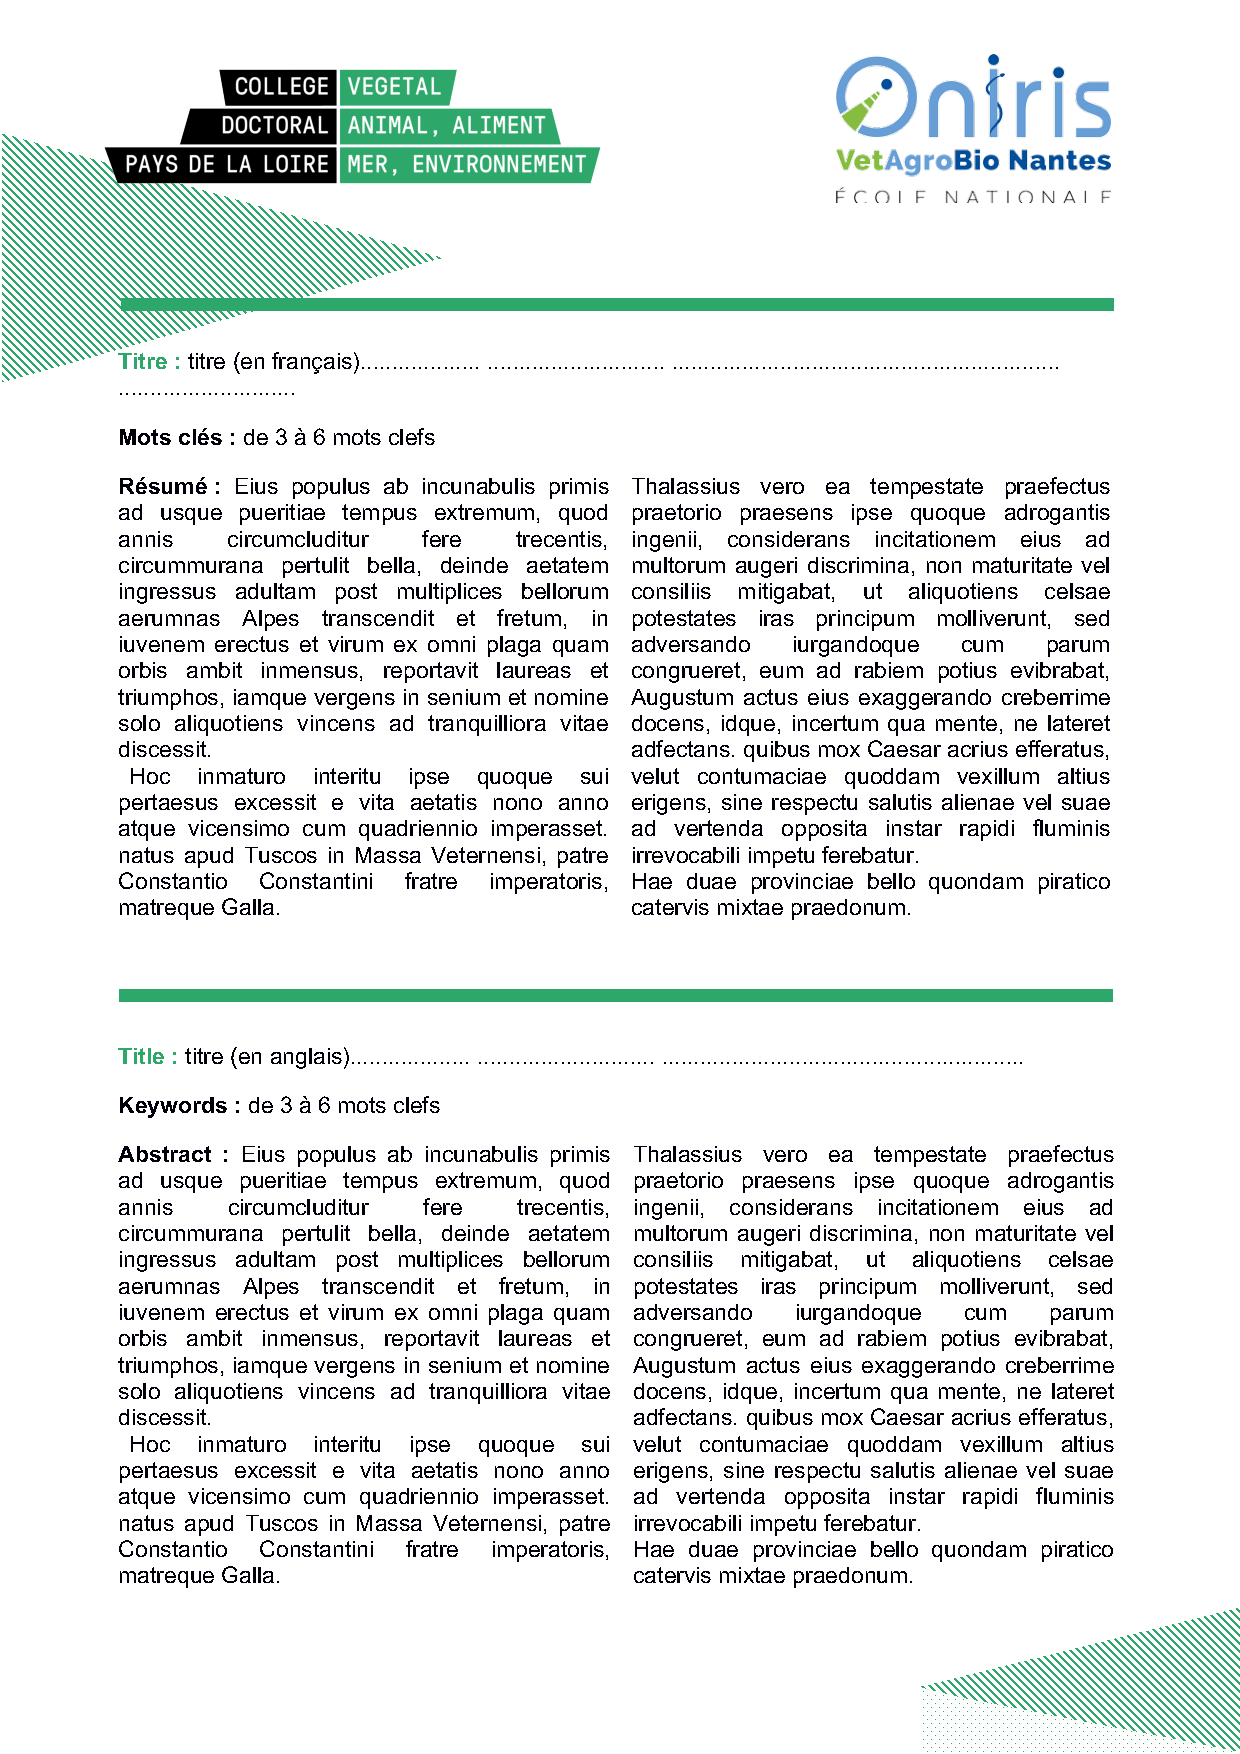
\includepdf[pages=1]{figures/ED_requirements/Abstract.pdf}

	
% \newpage
% \thispagestyle{empty}


% \mbox{}
% \newpage %résumé

\end{document}  
